\documentclass[12pt,a4paper]{report}


\usepackage{amsmath}
\usepackage[utf8]{inputenc}
\usepackage{amsmath}
%\usepackage{unicode-math}
\usepackage{amsfonts}
\usepackage{amssymb}
\usepackage{calrsfs}
\usepackage[left=2cm,right=2cm,top=2cm,bottom=2cm]{geometry}
\usepackage[mathscr]{euscript}

\usepackage{color}

%%%%%%%%%%%attach pdf%%%%%%%%%%%%
\usepackage[final]{pdfpages}
%%%%%%%%%%%%%%%%%%%%%%%%%%%%%%%%%

%%%%%%%%%%for writing large parallel%%%%%%
\usepackage{mathtools}
\DeclarePairedDelimiter\bignorm{\lVert}{\rVert}
%%%%%%%%%%%%%%%%%%%%%%%%%%%%%%%%%%%%%%%%%%

%%%%%%%%Draws Pretty Box%%%%%%%
%%%Use with \bluebox[<top pad>][<bot pad>]{<contents>}
\definecolor{myblue}{rgb}{.8, .8, 1}

\usepackage{empheq}

\newlength\mytemplen
\newsavebox\mytempbox

\makeatletter
\newcommand\bluebox{%
    \@ifnextchar[%]
       {\@bluebox}%
       {\@bluebox[0pt]}}

\def\@bluebox[#1]{%
    \@ifnextchar[%]
       {\@@bluebox[#1]}%
       {\@@bluebox[#1][0pt]}}

\def\@@bluebox[#1][#2]#3{
    \sbox\mytempbox{#3}%
    \mytemplen\ht\mytempbox
    \advance\mytemplen #1\relax
    \ht\mytempbox\mytemplen
    \mytemplen\dp\mytempbox
    \advance\mytemplen #2\relax
    \dp\mytempbox\mytemplen
    \colorbox{myblue}{\hspace{0em}\usebox{\mytempbox}\hspace{0em}}}
%%%%%%%%%%%%%%%%%%%%%%%%%%%%%%%%%%%%%%%%%%%%%

%%%%%%%%%%for writing symbol above an equality
\newcommand\xeq{\stackrel{\mathclap{\normalfont\mbox{d}}}{=}}
%%%%%%%%%%%%%%%%%%%%%%%%%%%%%%%%%%%%%%%%%%%%

%%%for drawing commutative diagrams.%%%%%%
\usepackage{tikz-cd}  
%%%%%%%%%%%%%%%%%%%%%%%%%%%%%%%%%%%%%%%%%%

%%%%%%%%%%%%%%double rules%%%%%%%%%%%%%%%%%%%
\usepackage{lipsum}% Just for this example

\newcommand{\doublerule}[1][.4pt]{%
  \noindent
  \makebox[0pt][l]{\rule[.7ex]{\linewidth}{#1}}%
  \rule[.3ex]{\linewidth}{#1}}
%%%%%%%%%%%%%%%%%%%%%%%%%%%%%%%%%%%%%%%%%%%%%%

%%%%%%%%%%for changing margin
\def\changemargin#1#2{\list{}{\rightmargin#2\leftmargin#1}\item[]}
\let\endchangemargin=\endlist 

\newenvironment{proof}
{\begin{changemargin}{1cm}{0.5cm} 
	}%your text here
	{\end{changemargin}
}

\newenvironment{subproof}
{\begin{changemargin}{0.5cm}{0.5cm} 
	}%your text here
	{\end{changemargin}
}
%%%%%%%%%%%%%%%%%%%%%%%%%%%%%

\begin{document}
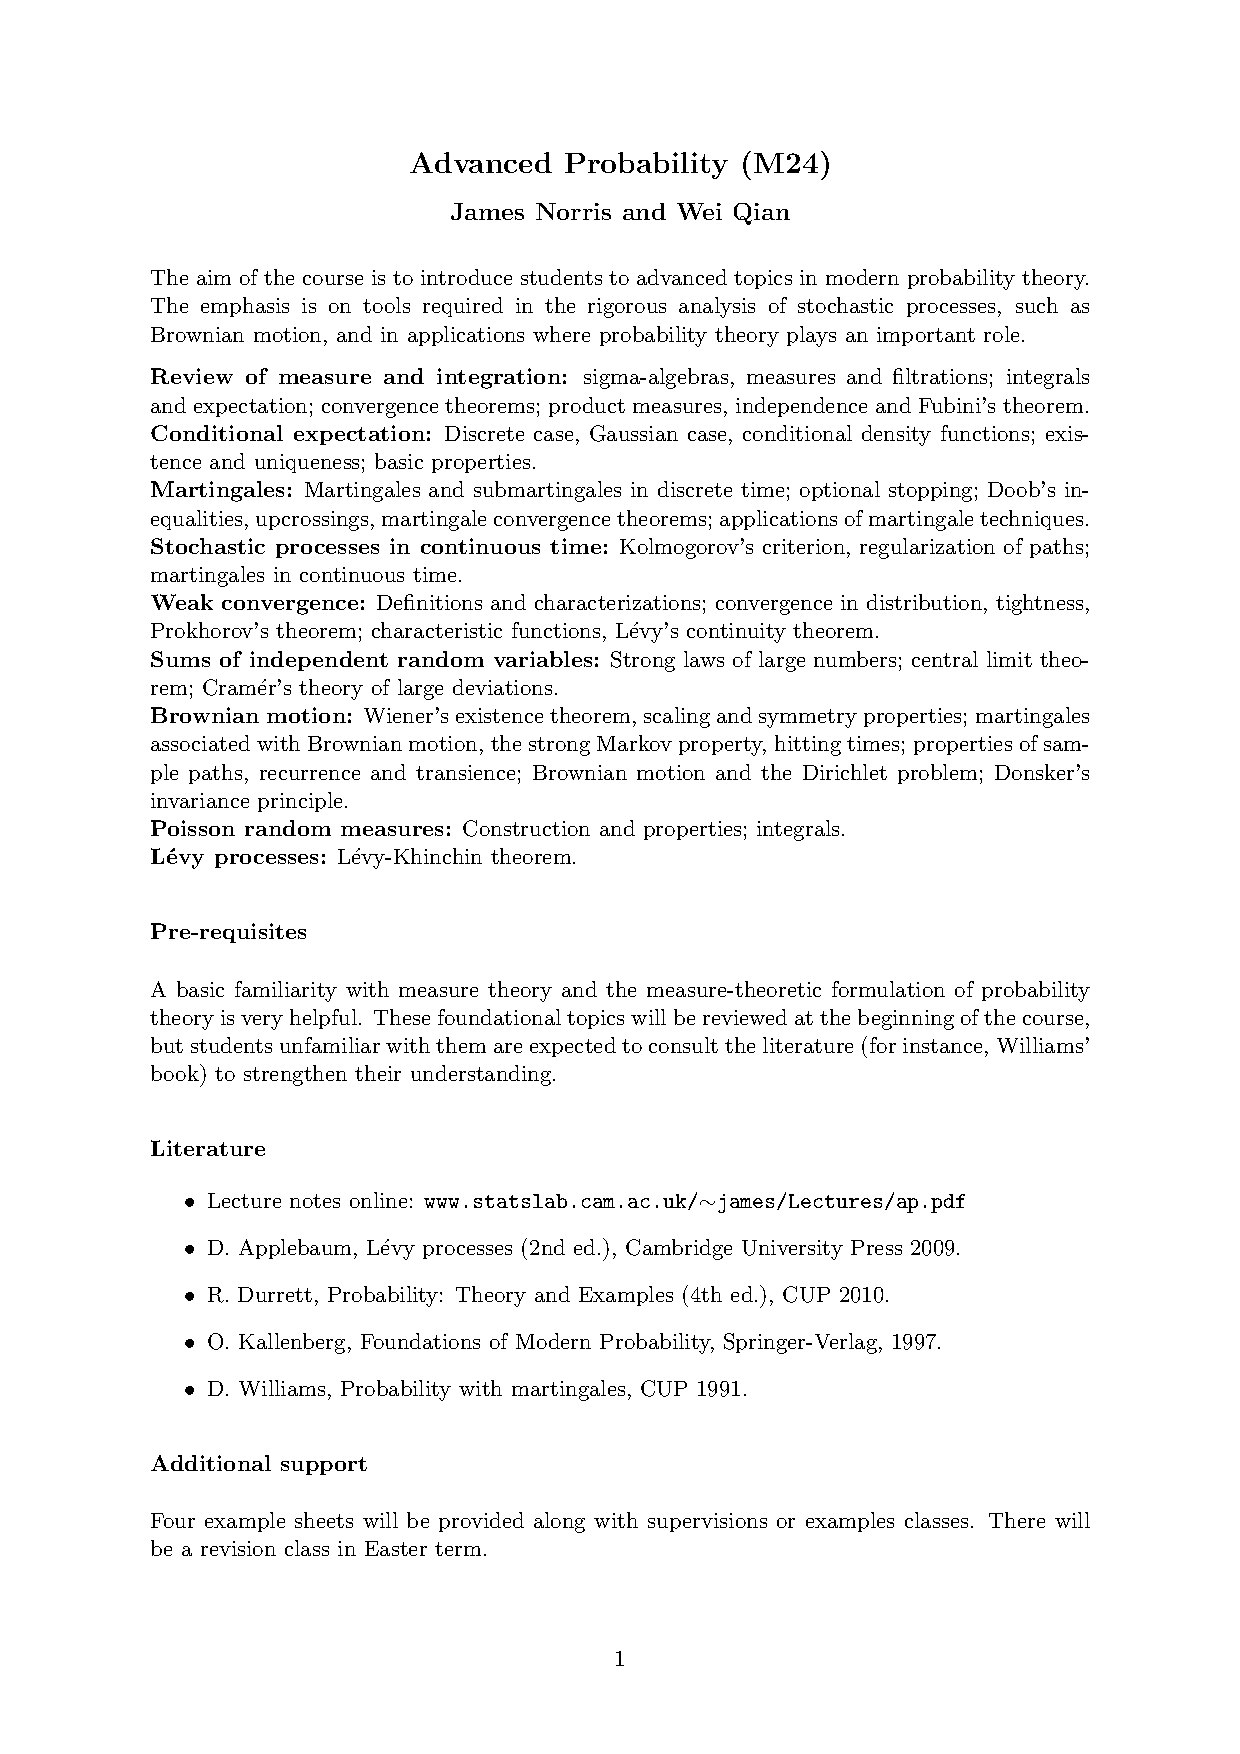
\includepdf{part-iii_probability_advanced-probability.pdf}

\newcommand{\thm}{\textbf{Theorem) }}
\newcommand{\thmnum}[1]{\textbf{Theorem #1) }}
\newcommand{\defi}{\textbf{Definition) }}
\newcommand{\definum}[1]{\textbf{Definition #1) }}
\newcommand{\lem}{\textbf{Lemma) }}
\newcommand{\lemnum}[1]{\textbf{Lemma #1) }}
\newcommand{\prop}{\textbf{Proposition)}}
\newcommand{\propnum}[1]{\textbf{Proposition #1) }}
\newcommand{\corr}{\textbf{Corollary) }}
\newcommand{\corrnum}[1]{\textbf{Corollary #1) }}
\newcommand{\pf}{\textbf{proof) }}


\newcommand{\lap}{\triangle} %%Laplacian
\newcommand{\s}{\vspace{10pt}}
\newcommand{\bull}{$\bullet$}
\newcommand{\sta}{$\star$}
\newcommand{\reals}{\mathbb{R}}

\newcommand{\eop}{\hfill  \textsl{(End of proof)} $\square$} %end of proof
\newcommand{\eos}{\hfill  \textsl{(End of statement)} $\square$} %end of proof


\newcommand{\intN}{\mathbb{Z}_N}
\newcommand{\nat}{\mathbb{N}}
\newcommand{\norms}[2]{\bignorm[\big]{#1}_{#2}}
\newcommand{\avg}{\mathbb{E}}
\newcommand{\prob}{\mathbb{P}}
\newcommand{\borel}{\mathscr{B}}
\newcommand{\EE}{\mathscr{E}}
\newcommand{\F}{\mathscr{F}}
\newcommand{\G}{\mathscr{F}}
\newcommand{\W}{\mathscr{W}}
\newcommand{\cov}{\text{Cov}}
\newcommand{\var}{\text{Var}}
\newcommand{\cha}{1}

\newcommand{\newday}{\doublerule[0.5pt]}

\setlength\parindent{0pt}

\chapter*{Advanced Probability}

Lectured by : Prof. James Norris(http://www.statslab.cam.ac.uk/$\sim$james/), Dr. Wei Qian

Example Classes given by : Peter Taylor, Piet Lammers
\s

Typed by : Jiwoon Park
\s

\begin{changemargin}{1.5cm}{1.5cm}
\textit{Some remarks :} This document was created during the lecture \textit{``Advanced Probability"}, Michaelmas term of 2018, University of Cambridge, Mathematics Tripos Part III. This is a 24-hours lecture course, and comes with 4 example sheets that can be found on http://www.statslab.cam.ac.uk/$\sim$james/Lectures/. This course is intended for students in first year of Masters degree in mathematics or equivalent. Background on elementary measure theory and functional analysis would be very helpful in this course.
\s

I tried to follow closely to the materials provided in the lecture, but minor modification also had been make. If there is any error in this notes, it is surely mine, and it has nothing to do with the lecturer or the university.
\s

This document was uploaded on http://www.github.com/ChocoUyou, along with its source code in \LaTeX. I hold no right on this document, and you are free to redistribute this document with any of its details below modified, but please do not just redistribute with any of the detail above this line modified.
\end{changemargin}

\newpage

\newday

(5th October 2018, Friday)

\section*{0. Review}

\subsection*{0.1. Measure Spaces}

Let $E$ be a set.
\s

Let $\EE$ be a set of subsets of $E$. We say that $\EE$ is a \textbf{$\sigma$-algebra} if $\phi \in \EE$ and for $A \in \EE$ and for any sequence $(A_n : n\in \mathbb{N})$ in $\EE$, we have $E\backslash A \in \EE$ and $\cup_n A_n \in \EE$. Then $(E,\EE)$ is called a \textbf{measurable space} and we call the elements of $\EE$ \textbf{measurable}.
\s

Let $\mu$ be a function $\EE \rightarrow [0,\infty]$. We say that $\mu$ is a \textbf{measure} if $\mu(\phi)=0$ and for all sequences $(A_n : n\in \mathbb{N})$ of disjoint elements, we have $\mu(\cup_n A_n) = \sum_n \mu(A_n)$.(\textbf{countable additivity}). The triple $(E,\EE, \mu)$ is called the \textbf{measure space}. 
\s

Given a topological space $E$ there is a smallest $\sigma$-algebra containing all the open sets. This is the \textbf{Borel $\sigma$-algebra}, denoted $\borel(E)$.
\s

E.g. For $\reals$, has $\borel(\reals) = \borel$, and $[0,\infty]$(the extended real positive line) has analogous Borel $\sigma$-algebra.
\s

\subsection*{0.2. Integration of Measurable Functions}

Let $(E, \EE)$ and $(E', \EE')$ be measurable spaces. A function $f: E \rightarrow E'$ is \textbf{measurable} if
\begin{align*}
f^{-1}(A) = \{ x\in E : f(x) \in A \} \in \EE \quad \forall A \in \EE'
\end{align*}

If we refer to a \textbf{measurable function} $f$ without specifying range, the default is $(\reals, \borel)$. 
\s

If we refer to $f$ as a \textbf{non-negative measurable function}, then we mean $E' = [0, \infty]$, $\EE' = \borel([0,\infty])$. Write $m\EE^+$ for the set of non-negative measurable functions.
\s

\thmnum{0.2.1.} Let $(E,\EE, \mu)$ be a measure space. Then there exists a \textit{unique} map $\tilde{mu} : m \EE^+ \rightarrow [0,\infty]$ such that
\begin{itemize}
\item[(a)] $\tilde{mu}(1_A) = \mu(A)$ for all $A \in \EE$.
\item[(b)] $\tilde{mu}(\alpha f + \beta g)= \alpha \tilde{mu}(f) + \beta \tilde{\mu}(g)$ for all $\alpha, \beta \in [0,\infty)$ and all $f,g \in m \EE^+$.
\item[(c)] (\textbf{monotone convergence}) $\tilde{\mu}(f) = \lim_{n\rightarrow \infty} \tilde{\mu}(f_n)$ for a non-decreasing sequence of functions $(f_n)_{n\in \mathbb{N}}$ in $m\EE^+$ such that $f_n(x) \rightarrow f(x)$ as $n\rightarrow \infty$ for all $x\in E$. 
\end{itemize}
\eos
\s

For now on, write $\mu$ for $\tilde{\mu}$. Call $\mu(f)$ the \textbf{integral of $f$} w.r.t. $\mu$. Also write $\int_E fd\mu = \int_E f(x) \mu(dx)$.
\s

A \textbf{simple function } is one which is a finite linear combination of indicator functions of measurable sets with positive coefficients. So $f$ is simple if $f = \sum_{k=1}^n \alpha_k 1_{A_k}$ for some $n \geq 0$, $\alpha_k \in (0,\infty)$ and $A_k \in \EE$ for $k\in \{1,\cdots, n\}$.
\s

Form (a) and (b) for $f$ simple, we have
\begin{align*}
\mu(f) = \sum_{k=1}^n \alpha_k \mu(A_k)
\end{align*}
Also, if $f,g \in m\EE^+$ with $f\leq g$ then $f+h = g$ where $h = g- f1_{f<\infty} \in m\EE^+$.  Since $\mu(h) \geq 0$, (b) implies $\mu(f) \leq \mu(g)$.
\s

Take $f\in m\EE^+$. Define for $x\in E$, $n \in \mathbb{N}$,
\begin{align*}
f_n(x) = 2^{-n}[2^n f(x)] \wedge n 
\end{align*}
Then $(f_n:n\in \mathbb{N})$ is a non-decreasing sequence of simple functions such that $f_n(x) \rightarrow f(x)$ for all $x\in E$. By monotone convergence(property (c)), we have
\begin{align*}
\mu(f) = \lim_{n\rightarrow \infty} \mu(f_n)
\end{align*}
These procedure characterizes $\mu(f)$ uniquely in terms of the measure $\mu : \EE \rightarrow [0,+\infty]$, (a), (b) and (c), so we have shown the uniqueness in \textbf{Theorem 0.2.1.}
\s

When is $\mu(f)=0$? (for $f\in m\EE^+$)
\s

For measurable functions $f,g$ we say $f=g$ \textbf{almost everywhere}(or a.e.) if
\begin{align*}
\mu(\{x\in E : f(x) \neq g(x) \}) =0
\end{align*}
Can show, for $f\in m\EE^+$, we have $\mu(f) =0$ if and only if $f=0$ a.e.
\s

Let $f$ be a measurable function. We say that $f$ is \textbf{integrable} if $\mu(|f|) <\infty$. Write $L^1 = L^1(E,\EE,\mu)$ for the set of all integrable functions. We extend the integral to $L^1$ by setting $\mu(f)= \mu(f^+) - \mu(f^-)$ where $f^{\pm}(x) = 0 \vee (\pm f(x))$ so that $f = f^+ + f^-$. Then can show $L^1$ is a vector space $\mu: L^1 \rightarrow \reals$ is linear. 
\s

\lemnum{0.2.2.} \textbf{(Fatou's lemma)} Let $(f_n:n\in \nat)$ be a sequence in $m\EE^+$. Then
\begin{align*}
\mu(\liminf_{n\rightarrow \infty} f_n) \leq \liminf_{n\rightarrow \infty} \mu(f_n)
\end{align*}
\eos

The proof is done by applying monotone convergence to the sequence $(\inf_{m\geq n} f_m : n \in \nat)$.
\s

\newday

(8th October, Monday)
\s

\thmnum{0.2.3}(Dominated Convergence) Let $(f_n :n \in \mathbb{N})$ be a sequence of measurable functions on $(E,\mathscr{E})$. Suppose $f_n(x) \rightarrow f(x)$ as $n\rightarrow$ for some function $f$ and for every $x\in E$. Suppose furthermore that $|f_n| \leq g$ for all $n$, for some measurable function $g$. Then $f_n$ is integrable for all $n$ and so is $f$. Moreover, we have $\mu(f_n) \rightarrow \mu(f)$ as $n\rightarrow \infty$.
\s

We call a measure space $(\Omega, \mathscr{F}, \mathbb{P})$ such that $\prob(\Omega) =1$ a \textbf{probability space}, with the following terms replaced:
\begin{align*}
\text{measurable functions} (f) &\leftrightarrow \text{random variable} (X) \\
\text{measurable sets} &\leftrightarrow \text{events} \\
\text{almost everywhere} &\leftrightarrow \text{almost surely}\\
\text{integral} & \leftrightarrow \text{expectation}(\avg{X} = \int_{\Omega} X d\prob \text{ in place of } \prob(X))
\end{align*}

\subsection*{0.3. Production measure and Fubini't theorem}

Take finite (or $\sigma$-finite) measure spaces $(E_1, \mathscr{E}_1, \mu_1)$ and $(E_2, \mathscr{E}_2, \mu_2)$. Write $\mathscr{E}_1 \otimes \mathscr{E}_2$ for the $\sigma$-algebra on $E_1 \times E_2$ generated by sets of the form $A_1 \times A_2$ for $A_1 \in \mathscr{E}_1$ and $A_2 \in \mathscr{E}_2$ and call this \textbf{product $\sigma$-algebra}.
\s

\thmnum{0.3.1.} There exists a unique measure $\mu = \mu_1 \otimes \mu_2$ on $(E_1 \times E_2, \mathscr{E}_1 \times \mathscr{E}_2)$ such that
\begin{align*}
\mu(A_1 \times A_2) = \mu_1(A_1) \mu_2(A_2) \quad \forall A_1 \in \mathscr{E}_1, A_2 \in \mathscr{E}_2
\end{align*}
\s

\thmnum{0.3.2.} (Fubini's theorem) Let $f$ be a non-negative measurable function on $(E_1 \times E_2, \mathscr{E}_1 \times \mathscr{E}_2)$.

\begin{itemize}
\item $x_1 \in E_1$, set $f_{x_1} (x_2) = f(x_1, x_2)$, then $f_{x_1}$ is $\mathscr{E_2}$-measurable for all $x_1 \in E_1$.

\item Set $f_1(x_1) = \mu_2(f_{x_1})$. Then $f_1$ is $\mathscr{E}_1$-measurable, and $\mu_1(f_1) = \mu(f)$.
\end{itemize} 
\eos

Now define $\hat{f}$ on $E_2 \times E_1$ by $\hat{f}(x_2,x_1) = f(x_1,x_2)$. Then we can show that $\hat{f}$ is $\mathscr{E}_2 \otimes \mathscr{E}_1$-measurable and $\mu_2 \otimes \mu_1 (\hat{f}) = (\mu_1 \otimes \mu_2)(f)$. So by Fubini, we have $\mu_2(f_2) = \hat{\mu}(\hat{f}) = \mu(f) \mu_1(f_1)$ where $f_2$ is defined as for $f_1$.
\s

i.e. $\int_{E_2} \big( \int_{E_1} f(x_1, x_2) \mu_1(dx_1) \big) \mu_2(dx_2) = \int_{E_1} \big( \int_{E_2} f(x_1, x_2) \mu_2(dx_2) \big) \mu_1(dx_1)$.
\s

Note, $f$ being integrable is also sufficient to for Fubini's theorem.
\s

\section*{Chapter 1. Conditional Expectation}
\subsection*{1.1. Discrete Case}

Suppose $(G_n : n\in \mathbb{N})$ is a sequence of disjoint sets in $\mathscr{F}$ such that $\cup_n G_n = \Omega$. Let $X$ be an integrable random variable.
\begin{itemize}
\item Set $\mathscr{G} = \sigma(G_n : n\in \mathbb{N}) = \{ \cup_{n\in I}G_n : I \subset \mathbb{N} \}$.

\item Define a new random variable $Y = \sum_{n \in \mathbb{N}} \avg(X | G_n ) 1_{G_n}$ where $\avg(X|G_n) =  \avg(X 1_{G_n}) / \prob(G_n)$ (used convention 0/0=0). Then,
\begin{itemize}
\item[(a)] $Y$ is $\mathscr{G}$-measurable.
\item[(b)] $Y$ is integrable and $\avg(Y 1_A) = \avg(X 1)A)$ for all $A \in \mathscr{G}$.
\end{itemize} 
We denote $Y = \avg(X|\mathscr{G})$ and call (a version of) the \textbf{conditional expectation} of $X$ given $\mathscr{G}$. 
\end{itemize}
\s

\subsection*{1.2. Gaussian Case}

Let $(W,X)$ be a Gaussian random variable in $\reals^2$ that has distribution $N(\mu, \Sigma)$. Take $\mathscr{G} = \sigma(W) = \{ W^{-1}(B) : B \in \mathscr{B}(\reals) \}$. 
\s

Consider, for $a,b \in \reals$, the random variable $Y = aW +b$.
\s

We can choose $a,b$ so that $\avg(Y)  = a\avg(X) + b = \avg(X)$ and $\cov(Y-X,W) = a \text{Var}(W) - \text{Var}(X,W) =0$. Then
\begin{itemize}
\item[(a)] $Y$ is $\mathscr{G}$-measurable.
\item[(b)] $Y$ is integrable and $\avg(Y 1_A) = \avg(X 1_A)$ for all $A \in \mathscr{G}$.
\end{itemize}
To see this, note $Y-X$ and $W$ are independent as $\cov(Y-X, W) =0$ so $\avg((Y-X)1_A) = \avg(Y-X) \prob(A) =0$ for all $A \in \mathscr{G}$.
\s

\subsection*{1.3. Conditional density functions}

Let $(U,V)$ be a random variable in $\reals^2$ with density function $f(u,v)$. That is, $\prob((U,V)\in A) = \int_A f(u,v)dudv$. Take $\mathscr{G} = \sigma(U) = \{ U^{-1}(B) : B \in \borel  \}$. Take a Borel measurable function $h$ on $\reals$ and set $X = h(V)$. Assume $X \in L^1(\prob)$. Note $U$ has density function $f(u) = \int f(u,v)dv$. Define the \textbf{conditional density function} $f(u|v) = f(u,v)/f(v)$(again with convention 0/0=0). Now set $Y=g(U)$ where $g(u) = \int_{\reals}h(v) f(v|u)dv$. Then $g$ is a Borel function on $\reals$ so
\begin{itemize}
\item[(a)] $Y$ is a $\mathscr{G}$-measurable random variable.
\item[(b)] $Y$ is integrable and for all $A = U^{-1}(B) \in \mathscr{G}$, we have $\avg(Y 1_A) = \avg(X 1_A)$.
\end{itemize}
To see this,
\begin{align*}
\avg(Y 1_A) &= \int_{\reals} g(u) 1_B (u) f(u) du \\
&= \int \int h(v) f(v|u) dv 1_B(u) f(u) du \\
&= \avg(X 1_A)
\end{align*}
using Fubini's theorem to go from second to the third line.
\s

\newday

(10th October, Wednesday)
\s

\subsection*{1.4. Existence and uniqueness of conditional expectation}

$(\Omega, \mathscr{F},\prob)$ is always the probability space behind.
\s

\thmnum{1.4.1.} Let $X$ be integrable random variable and let $\mathscr{G}$ be a sub-$\sigma$-algebra of $\mathscr{F}$. There exist a random variable $Y$ such that
\begin{itemize}
\item[(a)] $Y$ is $\G$-measurable,
\item[(b)] $Y$ is integrable and for all $A \in \G$, $\avg(Y1_A) = \avg(X1_A)$.
\end{itemize}
Moreover, if $Y'$ is another random variable satisfying (a) and (b) then $Y'=Y$ a.s.
\s

We will write $Y = \avg(X | \G)$ a.s.(because $\avg(X|\G)$ is not a fully specified random variable) and we say $Y$ is a \textbf{(version of) the conditional expectation of $X$ given $\G$}. In case $X = 1_A$ write $Y=\prob(A|\G)$ a.s.
\s

An analogous statement holds with 'integrable' replaced by 'non-negative' throughout the statement.
\begin{proof}
\pf \emph{(Uniqueness)} Suppose $Y$ satisfies (a) and (b), and $Y'$ satisfies (a) and (b) for an integrable random variable $X'$, with $X \leq X'$. Consider the non-negative random variable $Z = (Y-Y')1_A$ where $A = \{Y\geq Y'\} \in \G$. Then
\begin{align*}
\avg(Y1_A ) = \avg(X1_A) \leq \avg(X' 1_A) = \avg(Y' 1_A)
\end{align*} 
so $\avg(Z) \leq 0$ so $Z=0$ a.s. and so $Y\leq Y'$ a.s.

\quad By symmetry, if $X=X'$, we see that $Y=Y'$ a.s.

\emph{(Existence)} Consider for now the case $X \in L^2(\F)$ (that is, $\avg(|X|^2) <\infty$, which is stronger than being integrable). Since $L^2(\F)$ is a Hilbert space, and in fact $L^2(\G)$ is a closed subspace of $L^2(\F)$, there exists an orthogonal projection $Y$ of $X$ on $L^2(\G)$. That is, $Y \in L^2(\G)$ and for all $Z \in L^2(\G)$, we have $\avg((Y-X)Z) =0$. (This is because $(X-Y)$ should be orthogonal to $L^2(\G)$, and the inner product is given by $\langle X-Y, Z\rangle = \avg((X-Y)Z) =0$.) So for any $A\in \G$, take $Z = 1_A$ to see $\avg(Y1_A) = \avg(X1_A)$. So $Y$ satisfies (a) and (b).

\quad Suppose now that $X \geq 0$. Set $X_n = X \wedge n$ then $X_n \in L^2(\F)$. We have shown there exist $Y_n \in L^2(\G)$ such that for all $A \in \G$, we have $\avg(Y_n1_A) = \avg(X_n 1_A)$, $0\leq X_n \leq X_{n+1}$ and $0 \leq Y_n \leq Y$ for all $n$. Set $\Omega_0 = \{\omega \in \Omega : 0 \leq Y_n(\omega) \leq Y_{n+1}(\omega)$ for all $n \}$. Then $\prob(\Omega_0)=1$ (because it is a countable intersection of sets of measure 1). Define a non-negative $\G$-measurable random variable
\begin{align*}
Y_{\infty} =  \lim_{n\rightarrow \infty}  1_{\Omega_0} Y_n
\end{align*} 
Then $0 \leq 1_{\Omega_0} Y_n \nearrow Y_{\infty}$ as $n\rightarrow \infty$ so by monotone convergence, we have for all $A\in \G$
\begin{align*}
\avg(Y_{\infty} 1_A) = \lim_{n\rightarrow \infty} \avg(Y_n 1_A)  = \lim_{n\rightarrow \infty} \avg(X_n 1_A) = \avg(X 1_A)
\end{align*}
In particular, taking $A =\Omega$, we see $Y_{\infty}$ is integrable, so $\prob(Y_{\infty})=0$. So if we set $Y= Y_{\infty} 1_{Y_{\infty}<\infty}$, then $Y$ is a random variable and satisfies (a) and (b).

\quad In the general case we can apply the proceeding to $X^{\pm} = 0 \vee (\pm X)$ (so $X = X^+ - X^-$) to obtain $Y^{\pm}$ and then check $Y= Y^+ - Y^-$ satisfies (a) and (b).

\eop 
\end{proof}

\subsection*{1.5. Properties of conditional expectation}

Conditional expectations plays a central role in many core materials of the course. e.g. martingales and Brownian motion. So it would be useful to investigate some properties of conditional expectation.
\s

Fix an integrable random variable $X$ and sub-$\sigma$-algebra $\G$. \textbf{Theorem 1.4.1} has useful consequences:
\begin{itemize}
\item[(i)] $\avg (\avg(X|\G)) = \avg(X)$
\item[(ii)] If $X$ is $\G$-measurable then $\avg(X|\G) =X$ a.s.
\item[(iii)] If $X$ is independent of $\G$ then $\avg(X|\G) = \avg(X)$ a.s.
\begin{itemize}
\item[:] check for $A \in \G$, $\avg(X1_A) = \avg(X) \prob(A) = \avg(\avg(X)1_A)$ so $\avg(X)$ satisfies condition (b).
\end{itemize} 
\item[(iv)] If $X\geq 0$ a.s. then $\avg(X|\G) \geq 0$ a.s. (follows from the proof of \textbf{Theorem 1.4.1})
\item[(v)] For all $\alpha, \beta\in \reals$, all integrable random variables $X,Y$, has
\begin{align*}
\avg(\alpha X + \beta Y |\G) = \alpha \avg(X|\G) + \beta \avg(Y|\G) \quad \text{a.s.}
\end{align*}
\begin{itemize}
\item[:] check that the expression on the RHS satisfies condition (b) to show that it is a version of conditional expectation of $\alpha X + \beta Y$ given $\G$.
\end{itemize}
\s

Now consider a sequence of random variables $(X_n)_n$. 
\item[(vi)] \emph{(conditional monotone convergence)} If $0\leq X_n \nearrow X$ pointwise then $\avg(X_n |\G)\rightarrow \avg(X|\G)$ a.s.
\begin{itemize}
\item[:] To see this, we know $\avg(X_n|\G) \nearrow Y$ a.s. for some non-negative $\G$-measurable random variable $Y$. Take $A \in \G$ then by monotone convergence, we have
\begin{align*}
\avg(Y1_A)  &= \lim_{n\rightarrow \infty} \avg(\avg(X_n |\G) 1_A) \\
&= \lim_{n\rightarrow \infty} \avg(X_n 1_A) = \avg(X1_A)
\end{align*}
so $Y$ satisfies (b) for $X$.
\end{itemize} 
\item[(vii)] \emph{(Conditional Fatou's lemma)} For any non-negative random variables $X_n$,
\begin{align*}
\avg(\liminf_{n\rightarrow \infty} X_n |\G) \leq \liminf_{n\rightarrow \infty} \avg(X_n |\G)
\end{align*}

\begin{itemize}
\item[:] By conditional monotone convergence, we have
\begin{align*}
\avg(\liminf_{n\rightarrow \infty} X_n |\G) = \lim_{n\rightarrow \infty} \avg(\inf_{m\geq n} X_m |\G) &\leq \lim_{n\rightarrow \infty} \inf_{m\geq n} \avg(X_m | \G) \\
&= \liminf_{n\rightarrow \infty} \avg(X_n | \G)
\end{align*}
so we have the result.
\end{itemize}
\item[(viii)] \emph{(Conditional dominated convergence)} If $X_n(\omega) \rightarrow X(\omega)$ for all $\omega$ as $n\rightarrow \infty$ and there exist $Y$ integrable so $|X_n| \leq Y$ for all $n$, then 
\begin{align*}
\avg(X_n|\G) \rightarrow \avg(X|\G) \quad \text{a.s.}
\end{align*}
\begin{itemize}
\item[:] First, note that $X_n$ and $X$ are integrable, since they are bounded by $Y$. Consider the sequence of non-negative random variables $Z_n = Y-X_n$. By Fatou's lemma,
\begin{align*}
\avg(\liminf_{n} Z_n |\G) = \avg(Y-X|\G) \leq \liminf_{n} \avg(Y-X_n|\G) = \avg(Y|\G) - \limsup_{n} \avg(X_n|\G)
\end{align*}
and hence
\begin{align*}
\limsup_{n} \avg(X_n|\G) \leq \avg(X|\G)
\end{align*}
On the other hand, if we let $W_n = Y+X_n$, applying Fatou's lemma gives
\begin{align*}
\avg(\liminf_n W_n |\G) = \avg(Y|\G) + \avg(X|\G) \leq \avg(Y|\G) + \liminf_{n} \avg(X_n|\G)
\end{align*}
and so
\begin{align*}
\liminf_n \avg(X_n|\G) \geq \avg(X|\G)
\end{align*}
The two inequalities give the result.
\end{itemize}
\end{itemize}

\newday

(12th October, Friday)
\s

\begin{itemize}
\item[(ix)] \emph{(Conditional Jensen)} Let $c: \reals \rightarrow (-\infty, \infty]$ be convex. Then $c(\avg(X|\G)) \leq \avg( c(X) |\G)$ a.s.
\begin{itemize}
\item[:] To see this, since $c$ is convex there exist real sequences $(a_n)$,$(b_n)$ such that $c(x) = \sup_n (a_n x +b_n)$. Then $c(X) \geq a_n X +b_n$ for all $n$. So
\begin{align*}
\avg(c(X)|\G) \geq \avg(a_n X + b|\G) = a_n \avg(X|\G) + b_n \quad \text{a.s.}
\end{align*}
so $\avg(c(X)|\G) \geq c(\avg(X|\G))$ a.s.
\end{itemize}
\item[(x)] $\norms{\avg(X|\G)}{p}\leq \norms{X}{p}$ for all $p\in [0,\infty)$ (where $\norms{X}{p} = \avg(|X|^p)$)
\begin{itemize}
\item[:] To see this, take $c(x) = |x|^p$ in conditional Jensen's inequality.
\end{itemize}
\item[(xi)] \emph{(Tower property)} This is also important for martingales.

Suppose $\mathscr{H} \subset \G \subset \F$ be sub-$\sigma$-algebras. Then
\begin{align*}
\avg(X|\mathscr{H}) = \avg(\avg(X|\G)|\mathscr{H}) \quad \text{a.s.}
\end{align*}
\begin{itemize}
\item[:] Proof is an exercise.
\end{itemize}
\item[(xii)] \emph{(Taking out what is known)} This is related to the 'filtration' that is to be introduced in the theory of martingales.

Let $Y$ be a bounded $\G$-measurable random variable. Then 
\begin{align*}
\avg(YX|\G)  = Y\avg(X|\G) \quad \text{a.s.} \quad \cdots\cdots (\star)
\end{align*}
\begin{itemize}
\item[:] To see this, consider first the case when $Y=1_B$, $B\in \G$. Take $A\in \G$, then
\begin{align*}
\avg(Y\avg(X|\G) 1_A) = \avg(\avg(X|\G)1_A) = \avg(X1_{AB)} = \avg(YX1_A) 
\end{align*}
so above identity $(\star)$ holds. The general case follows by a monotone class argument. i.e. ($\star$) extends by linearity to case where $Y$ is simple. Next consider $X,Y\geq 0$ and set $Y_n = (2^{-n} \lfloor 2^n \rfloor)\wedge n$. Then $Y_n$ is simple, so $\avg(Y_n X 1_A) = \avg(Y_n \avg(X|\G))$ for all $A\in \G$. Let $n\rightarrow \infty$ using monotone convergence to obtain ($\star$) for $Y$. Finally extend to $X,Y$ general using $X = X^+ - X^-$ and $Y=Y^+ - X^-$.(Or instead, use \emph{monotone class theorem}, that abstracts this process)
\end{itemize}
\item[(xiii)] Let $\mathscr{H}$ be a $\sigma$-algebra and suppose $\mathscr{H}$ is independent of $\sigma(X,\G)$. Then
\begin{align*}
\avg(X|\sigma(\G, \mathscr{H})) = \avg(X|\mathscr{H}) \quad \text{a.s.}
\end{align*}
\begin{itemize}
\item[:] To see this, put $Z =\avg(X|\sigma(\G, \mathscr{H}))$ and $Y = \avg(X|\mathscr{H})$. Take $A\in \G$, $B\in \mathscr{H}$.
\begin{align*}
&\avg(Y 1_{A\cap B}) = \avg(X 1_A 1_B)= \avg(X1_A)\prob(B) \\
=& \avg(Y1_A) \prob(B) = \avg(Y1_{A\cap B})
\end{align*}
Hence $\avg((Z-Y)1_{A\cap B})= 0$ for all $A\in \G$, $B\in \mathscr{H}$. Also, $(Z-Y)$ is $\sigma(\G,\mathscr{H})$-measurable, and therefore $Y=Z$ by standard argument, e.g. using the following lemma.
\begin{itemize}
\item[] \lem Suppose $X$ is integrable and $\avg(X1_A) = 0$ for all $A\in \mathscr{A}$ where $\mathscr{A}$ is a $\pi$-system generating $\F$. Then $X=0$ a.s.

\pf Consider $\mathscr{D}  = \{A\in \F : \avg(X1_A) =0\}$ then $\mathscr{D}$ is a $d$-system, contains $\mathscr{A}$ so $\mathscr{D} = \F$ by Dynkin's lemma. Finally, $\avg(X 1_{ \{X>0}\} ) =0$ so $X=0$ a.s.
\end{itemize}
\end{itemize}
\end{itemize}
\s

We end the chapter with a lemma that is going to be useful.
\s

\lemnum{1.5.1.} Let $X\in L^1(\prob)$. Set $\mathcal{Y} = \{\avg(X|\G) : \G \subset \F$ a sub-$\sigma$-algebra $\}$. Then $\mathcal{Y}$ is UI(\emph{uniformly integrable}). That is,
\begin{align*}
\sup_{Y \in \mathcal{Y}} \avg(|Y| 1_{|Y|\geq \lambda}) \rightarrow 0 \quad \text{as } \lambda \rightarrow \infty
\end{align*}
\begin{proof}
\pf Since $X$ is integrable, given $\epsilon >0$, there exists $\delta>0$ s.t. $\avg(|X| 1_A) \leq \epsilon$ whenever $\prob(A) \leq \delta$. (Suppose not, then we should find $\epsilon>0$ and $A_n \in F$ s.t. $\prob(A_n) \leq 2^{-n}$ and $\avg(|X|1_{A_n}) >\epsilon$. Set $A= \bigcap_n \bigcup_{m\geq n} A_m$. Then $\prob(A) =0$ by Borel-Cantelli lemma. But $\avg(|X| 1_{\cup_{m\geq n} A_m}) \geq \epsilon$, while this converges to $\avg(|X|1_A) =0$ as $n\rightarrow \infty$, which is a contradiction.)

\quad Choose $\lambda \in (0,\infty)$ so that $\avg(|X|) \leq \lambda \delta$. Take $Y = \avg(X|\G) \in \mathcal{Y}$. Since $x\mapsto |x|$ is a convex function, by conditional Jensen's inequality,
\begin{align*}
Y \leq \avg(|X| |\G) \quad \text{so} \quad \avg(|Y|) \leq	\avg(|X|)
\end{align*}
(In fact, by decomposition $X= X^+ + X^-$, we see that $|Y| = \avg(X^+ | \G) + \avg(X^-|\G)) = \avg(|X|\big| \G)$ a.s.... but does not need this at this point)

By Chebyshev's inequality, $\prob(|Y|\geq \lambda) \leq \lambda^{-1} \avg(|Y|)\leq \delta$ hence
\begin{align*}
\avg\Big( |Y| 1_{|Y|\geq \lambda} \Big) &\leq \avg\Big( \avg(|X||\G) 1_{|Y|\geq \lambda} \Big) \quad \text{as } 1_{Y\geq \lambda} \in \G \\
&= \avg  (|X| 1_{|Y|\geq \lambda}) \leq \epsilon
\end{align*}
So $\sup_{x\in \mathcal{Y}} \avg(|Y|1_{|Y|\geq \lambda}) \leq \epsilon$. This is true for any $\epsilon>0$, therefore we have the uniform integrability.

\eop
\end{proof}
\s

\newday

(15th October 2018, Monday)
\s

\section*{Chapter 2. Martingales in Discrete Time}

\subsection*{2.1. Definitions.}

Let $(\Omega, \F, \prob)$ be a probability space.


\begin{itemize}
\item A \textbf{Filtration} for $(\Omega, \F, \prob)$ is a sequence $(\F_n)_{n\geq 0}$ of $\sigma$-algebras s.t. for all $n \geq 0$, we have
\begin{align*}
\F_n\subset \F_{n+1} \subset \F
\end{align*}
Set $F_{\infty} = \sigma(\F_n:n\geq 0)$ then $\F_{\infty} \subset \F$. We allow $\F_{\infty} \neq \F$. We interpret $n$ as times and $\F_n$ as the extent of knowledge at time $n$.

\item A \textbf{Random process(in discrete time)} is a sequence of random variables $(X_n)_{n\geq 0}$. It has a natural filtration $(F_n^X)_{n\geq 0}$ given by
\begin{align*}
\F_n^X = \sigma(X_0, \cdots, X_n)
\end{align*}
That is, the knowledge obtained from $X_n$ by time $n$. We say $(X_n)_{n\geq 0}$ is \textbf{adapted to} $(\F_n)_{n\geq 0}$ if $X_n$ is $\F_n$-measurable for all $n\geq 0$. This is equivalent to having $\F_n^X \subset \F_n$, for all $n \geq 0$. (Here, $X_n$ are real-valued) 

\item We would say $(X_n)_{n\geq 0}$ is \textbf{integrable} if $X_n$ is integrable for all $n\geq 0$.

\item A \textbf{martingale} is an \emph{adapted, integrable random process} $(X_n)_{n\geq 0}$ s.t. for all $n\geq 0$,
\begin{align*}
\avg[X_{n+1} |\F_n] = X_n \quad \text{a.s.}
\end{align*}
In the case $\avg[X_{n+1} |\F_n] \leq X_n$ a.s., $(X_n)_n$ is called a \textbf{super-martingale} and in the case $\avg[X_{n+1} |\F_n] \geq X_n $ a.s., $(X_n)_n$ is called a \textbf{sub-martingale}.
\end{itemize}

\newcommand{\randp}{(X_n)_{n \geq 0}} %a random process

\subsection*{Optional Stopping}

\begin{itemize}
\item A random variable $T:\Omega \rightarrow \{ 0,1,2,\cdots \} \cup \{\infty\}$ is a \textbf{stopping time} if $\{ T\leq n\}\in \F_n$ for all $n \geq 0$.

\item For a stopping time $T$, we set $\F_T = \{ A\in \F_{\infty} : A\cap \{ T\leq n \} \in \F_n$ for all $n\geq 0 \}$. It is easy to check $\F_T$ is indeed a $\sigma$-algebra and that if $T(\omega) = n$ for all $\omega \in \Omega$, then $T$ is a stopping time and $\F_T = \F_n$.

\item Given $X$, define $X_T(\omega) = X_{T(\omega)}(\omega)$ whenever $T(\omega) <\infty$ and define the \textbf{stopped process} $X^T$ by
\begin{align*}
X_n^T (\omega)  = X_{T(\omega) \wedge n} (\omega) \quad \text{for } n\geq 0
\end{align*}
\end{itemize}

\propnum{2.2.1.} Let $X$ be an adapted process. Let $S$, $T$ be stopping times for $X$. Then
\begin{itemize}
\item[(a)] $S\wedge T$ is a stopping time for $X$.
\item[(b)] $\F_T$ is a $\sigma$-algebra.
\item[(c)] If $S\leq T$ then $\F_S \subset \F_T$.
\item[(d)] $X_T 1_{T<\infty}$ is an $\F_T$-measurable random variable.
\item[(e)] $X^T$ is adapted.
\item[(f)] If $X$ is integrable, then $X^T$ is also integrable.
\end{itemize}

\begin{proof}
\pf
\begin{itemize}
\item[(a)] $\{ S \wedge T \leq n \} = \{S  \leq n \} \cup \{ T \leq n\} \in \F_n$ for all $n\geq 0$, so $S\wedge T$ is a stopping times

\item[(b)] Directly from the definition, we see that $\phi \F_T$. Also, given $A\in \ \F_T$ and a sequence $(A_m)_m \subset \F_T$, we have
\begin{align*}
& A^c \cap \{T\leq n \} = \{T\leq n\} - A \cap \{T\leq n \} \in \F_n \quad \Rightarrow  A^c \in \F_T \\
&(\cup_m A_m) \cap \{T\leq n\} =  \cup_m (A_m \cap \{T\leq n\}) \in \F_n \quad \Rightarrow \cup_m A_m \in \F_T
\end{align*}
hence $\F_T$ is a $\sigma$-algebra.

\item[(c)] Let $A\in \F_S$. Then $A\cap \{T\leq n\} = A \cap \{S\leq n\} \cap \{T \leq n\} \in \F_n$, hence $A \in \F_T$.

\item[(d)] For each $t\in \reals$, we have $\{X_T 1_T >t \} = \cup_m \{X_m >t, T=n \}$ so for any $n\geq 0$,
\begin{align*}
\{X_T 1_T >t \} \cap \{T\leq n\} = \cup_{m=1}^n \{X_m >t, T=n \} \in \F_n
\end{align*}
and so $X_T 1_T$ is $\F_T$-measurable.

\item[(e)] By definition of being a stopping time, for any $t\in \reals$, 
\begin{align*}
\{(X^T)_n >t\} = \{T>n, X_n>t\} \cup \Big( \cup_{m=0}^n \{T=m, X_m>t \} \Big)\in \F_n
\end{align*}
so $X^T$ is adapted.

\item[(f)] First consider the case where $X$ is non-negative integrable. Then
\begin{align*}
\avg(X^T_n) = \avg(\avg(X_n^T |T)) = \sum_{m\geq n} \prob(T=m) \avg(X_m) + \prob(T>n) \avg(X_n) < \infty
\end{align*}
for any $n$, so we have the result for non-negative $X$.

\quad For the general case, divide $X$ into a non-negative and a negative part.
\end{itemize}
\eop
\end{proof}
\s

\thmnum{2.2.2} \emph{(Optional stopping theorem)} Let $X$ be a super-martingale and let $S,T$ be \emph{bounded} stopping times with $S \leq T$ a.s. Then
\begin{align*}
\avg[X_T] \leq \avg[X_S]
\end{align*}
\begin{proof}
\pf Fix $n\geq 0$ such that $T\leq n$ a.s. Then
\begin{align*}
X_T &= X_S + \sum_{S\leq k <T} X_{k+1} - X_k  \\
&= X_S + \sum_{k=0}^n (X_{k+1} - X_k) 1_{S\leq k <T}
\end{align*}
Now $\{S\leq k\}$ is in $\F_k$ and $\{T>k\}$ is in $\F_k$, so
\begin{align*}
\avg[(X_{k+1} - X_k)1_{S\leq k <T}  ] &= \avg [\avg[ (X_{k+1} - X_k) 1_{S\leq k<T} |\F_k ]] \\
& = \avg[ \avg [  X_{k+1} -X_k | \F_k ] 1_{S\leq k < T} ]
\end{align*}
but since $(X_n)$ was a super-martingale,  $\avg [  X_{k+1} -X_k | \F_k ] \leq 0$ a.s. and therefore $\avg[(X_{k+1} - X_k)1_{S\leq k <T}  ] \leq 0$ a.s. Hence $\avg(X_T) \leq \avg(X_S)$.

\eop
\end{proof}
\s

$\star$ Note that $X$ is a sub-martingale \emph{if and only if} ($-X$) is a super-martingale, and that $X$ is a martingale \emph{if and only if} $X$ and ($-X$) are super-martingales. Hence, we obtain sub-martingale and martingale versions of the theorem :
\begin{align*}
&\text{If } (X_n) \text{ is a sub-martingale, } \avg[X_T] \geq \avg[X_S] \\
&\text{If } (X_n) \text{ is a martingale, } \avg[X_T] = \avg[X_S]
\end{align*}
\s

\thmnum{2.2.3.} Let $X$ be an adapted integrable process. Then the followings are equivalent.
\begin{itemize}
\item[(a)] $X$ is a super-martingale. 
\item[(b)] for all bounded stopping times $T$ and stopping time $S$,
\begin{align*}
\avg(X_T |\F_S) \leq X_{S\wedge T} \quad \text{a.s.},
\end{align*}
\item[(c)] for all stopping times $T$, the stopped process $X^T$ is a super-martingale,
\item[(d)] for all bounded stopping times $T$ and all stopping times $S$ with $S\leq T$ a.s,
\begin{align*}
\avg(X_T) \leq \avg(X_S)
\end{align*}
\end{itemize}

$\star$ The theorem gives an inverse statement of the optional stopping theorem.
\s

\begin{proof}
\pf

\begin{itemize}
\item[(a) $\Rightarrow$ (b)] Suppose $X$ is a super-martingale and $S,T$ are stopping times. Let $T\leq n$, for some $n<\infty$. Then
\begin{align*}
X_T = X_{S\wedge T} + \sum_{k=0}^T (X_{k+1} - X_k) 1_{S\leq k<T} \cdots \cdots (*)
\end{align*}
Let $A \in \F_S$. Then $A\cap \{ S\leq k\}\in \F_k$ and $\{T>k\} \in \F_k$ so
\begin{align*}
\avg[(X_{k+1} - X_k) 1_{S\leq k<T} 1_A] =\avg[\avg[(X_{k+1} - X_k) 1_{S\leq k<T} 1_A|\F_k]] \leq 0
\end{align*}
and
\begin{align*}
\avg[(X_T - X_{S\wedge T}) 1_A] = & \avg[\sum_{n=0}^T (X_{k+1} - X_k) 1_{S\leq k<T} 1_A] \leq 0 \\
& \Rightarrow \quad \avg[ X_T 1_A] \leq \avg[X_{S\wedge T} 1_A] \\
\end{align*}
But since this inequality is true for any $A\in \F_S$ and noting that $X_{S\wedge T} \in \F_S)$, we see
\begin{align*}
\avg[X_T |\F_S] \leq X_{S\wedge T} \quad \text{a.s.}
\end{align*}
\s

The implications (b)$\Rightarrow$(c) and (c)$\Rightarrow$(d) are obvious.
\s

\item[(d) $\Rightarrow$ (a)] Let $m\leq n$ and $A\in \F_n$. Set $T= m1_A + n1_{A^c}$. Then $T$ is a stopping with $T\leq n$. Then
\begin{align*}
\avg(X_n 1_A -X_m 1_A) = \avg(X_n) - \avg(X_T) \leq 0
\end{align*}
(note, if $\omega \in A$ then $(X_n1_A - X_m1_A)(\omega) = X_n(\omega) -X_m(\omega)$ and $0$ otherwise) so
\begin{align*}
\avg[X_n | \F_m] \leq X_m
\end{align*}
\end{itemize}
\eop
\end{proof}
\s

\newday

(17th October, Wednesday)
\s

\subsection*{2.3. Doob's upcrossing inequality}

\begin{itemize}
\item Let $X$ be a random process and let $a,b\in \reals$ s.t. $a<b$. Fix $\omega \in \Omega$. By an \textbf{upcrossing} of $[a,b]$ by $X(\omega)$, we mean an interval of times $\{j,j+1, \cdots, k\}$ s.t. $X_j(\omega) <a$, $X_k(\omega) >b$.

\item Write $U_n[a,b](\omega)$ for the number of disjoint upcrossings contained in $\{0,1,\cdots,n\}$, and $U_n[a,b] \nearrow U[a,b]$ as $n\rightarrow \infty$.
\end{itemize}
\s


\begin{figure}[h]
	\centering
		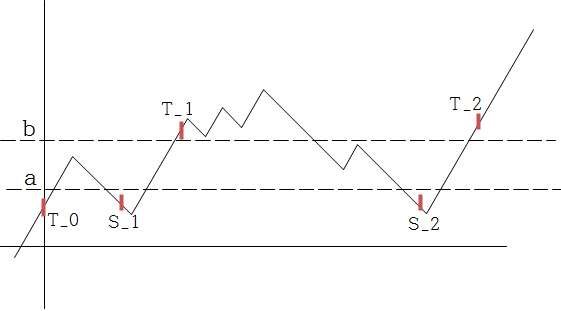
\includegraphics[scale=0.5]{upcrossing}
	\centering
\end{figure}


\thmnum{2.3.1.}(Doob's upcrossing inequality) Let $X$ be a \emph{super-martingale}. Then
\begin{align*}
(b-a) \avg[U[a,b]] \leq \sup_{n\geq 0} \avg[(X_n-a)^{-}]
\end{align*}
(Recall, $x^- = (-x) \vee 0$)
\s

In fact, in this theorem, we prove $(b-a) \avg[U_n[a,b]] \leq  \avg[(X_n-a)^{-}]$.
\begin{proof}
\pf Set $T_0 =0$ and define recursively for $k\geq 0$,
\begin{align*}
S_{k+1} = \inf \{m\geq T_k : X_m <a \}, \quad T_{k+1} = \sup \{m\geq S_{k+1} : X_m >b \}
\end{align*}
Note that if $T_k < \infty$, then $\{S_k, S_{k}+1,\cdots, T_k \}$ is an upcrossing of $[a,b]$ by $X$, and $T_k$ is the time of completion of the $k-th$ upcrossing. Also note that $U_n [a,b] \leq n$. For $m\leq n$, we have
\begin{align*}
\{U_n[a,b] =m \} = \{T_m \leq n < T_{m+1} \}
\end{align*}
On this event,
\begin{align*}
X_{T_k \wedge n}  - X_{S_k \wedge n} = \begin{cases}
X_{T_k} - X_{S_k} \geq b-a \quad \text{if } k\leq m \\
X_n - X_{S_k} \geq X_n -a \quad \text{if } k \geq m+1, S_{m+1} \leq n \\
0 \quad \text{otherwise}
\end{cases}
\end{align*}
Hence
\begin{align*}
\sum_{k=1}^n (X_{T_k \wedge n} - X_{S_k \wedge n}) &\geq (b-a) U_n[a,b] + X_n - a \\
&\geq (b-a)U_n[a,b] -(X_n -a)^-
\end{align*}
Since $X$ is a super-martingale and $T_k \wedge n$ and $S_k \wedge n$ are \emph{bounded stopping times} with $S_k \leq T_k$, by optional stopping theorem, we have
\begin{align*}
\avg (X_{T_k \wedge n})\leq \avg(X_{S_k \wedge n})
\end{align*}
By $\avg(\sum_{k=1}^n (X_{T_k \wedge n} - X_{S_k \wedge n})) \leq 0$ we get
\begin{align*}
(b-a) \avg(U_n[a,b]) \leq  \avg[(X_n-a)^-]
\end{align*}
Apply monotone convergence, with $n\rightarrow \infty$, then we are done.

\eop
\end{proof}
\s

This theorem does not seem to have any significance at the moment, but it will turn out to be important later on.

\subsection*{2.4. Doob's maximal inequalities.}

\quad Define $X_n^* = \sum_{k\geq n} |X_k|$
\s

In the next two theorems, we see that the martingale(or sub-martingale) property allows us to obtain estimates on this $X_n^*$ in terms of expectations for $X_n$.\\
\s

\thmnum{2.4.1} (Doob's maximal inequality) Let $X$ be a \emph{martingale or a non-negative sub-martingale}. Then for all $\lambda \geq 0$,
\begin{align*}
\lambda \prob(X_n^* \geq \lambda) \leq \avg(|X_n|   1_{\{ X_n^*\geq \lambda \}}) \leq \avg(|X_n|)
\end{align*}
\begin{proof}
\pf If $X$ is a martingale, then $|X|$ is a non-negative sub-martingale. It suffices to consider the case where $X$ is a non-negative sub-martingale.

\quad Set $T = \inf \{ k \geq 0 : X_k \geq \lambda \} \wedge n$. Then $T$ is a stopping time and $T\leq n$, so by optional stopping, has
\begin{align*}
\avg(X_n) \geq \avg(X_T) &= \avg(X_T 1_{X^*_n \geq \lambda}) + \avg(X_T 1_{X^*_n < \lambda}) \\
& = \avg( \lambda 1_{X^*_n \geq \lambda})  + \avg(X_n 1_{X_n^* < \lambda})
\end{align*}
and
\begin{align*}
\avg(X_n 1_{X^* \geq \lambda}) \geq \lambda \prob(X^*_n \geq \lambda)
\end{align*}

\eop
\end{proof}
\s

\thmnum{2.4.2} (Doob's $L^p$-inequality) Let $X$ be a \emph{martingale or a non-negative sub-martingale}. Then, for all $p>1$ and $q = p/(p-1)$, we have
\begin{align*}
\norms{X^*_n}{p} \leq q \norms{X_n}{q} 
\end{align*}
\begin{proof}
\pf Again, it suffices to consider when $X$ is a non-negative sub-martingale. Fix $k < \infty$. Then
\begin{align*}
\avg [ (X^*_n \wedge k)^p  ] &= \avg \int_0^k p \lambda^{p-1} 1_{\{x^*_n \lambda \}} d\lambda \quad \text{(integration by parts)}\\
& = \int_0^k p \lambda^{p-1} \prob(X^*_n \geq \lambda) d\lambda \quad \text{(Fubini)} \\
& \leq \int+0^k p\lambda^{p-2} \avg (X_n 1_{X^*_n \geq \lambda}) d\lambda \quad \text{(Doob's maximal inequaltiy)} \\
& =\frac{p}{p-1} \avg(X_n (X^*_n \wedge k)^{p-1} ) \\
& \leq q \norms{X_n}{p} \norms{X^*_n \wedge k}{p}^{p-1} \quad \text{(H\"{o}lder's inequality)}
\end{align*}
Hence , $\norms{X^*_n \wedge k}{p} \leq q\norms{X_n}{p}$. Apply monotone convergence theorem with $k\rightarrow \infty$, then we have the desired result.

\eop
\end{proof}
\s

Doob's maximal and $L^p$ inequalities have different versions which apply under the same hypothesis to
\begin{align*}
X^* = \sum_{n\geq 0} |X_n|
\end{align*}
since $X^*_n \nearrow X^*$. Letting $n\rightarrow \infty$ in Doob's maximal inequality gives
\begin{align*}
\lambda \prob(X^* \geq \lambda) \lim_{n\rightarrow \infty} \lambda \prob(X^*_n \geq \lambda) \leq \sup_{n\geq 0} \avg(|X_n|)
\end{align*}
We can then replace $\lambda \prob(X^* >\lambda)$ by $\lambda \prob (X^* \geq \lambda)$ by taking limits from the right in $\lambda$.

\quad Similarly, for $p\in (1,\infty)$ by monotone convergence,
\begin{align*}
\norms{X^*}{p} \leq q \sup_{n\geq 0} \norms{X_n}{p}
\end{align*}
\s

\newday

(19th October, Friday)
\s

\subsection*{2.5. Doob's martingale convergence theorems}

We are going to study three different martingale convergence theorems. They are all important.
\s

\begin{itemize}
\item We say that a random process $X$ is \textbf{$L^p$-bounded} if $\sum_{n\geq 0} \norms{X_n}{p} <\infty$.
\item We say that $X$ is \textbf{uniformly integrable} if
\begin{align*}
\sup_{n\geq 0} \avg (| X_n | 1_{|X_n| >\lambda})\rightarrow 0 \quad \text{as }\lambda \rightarrow \infty
\end{align*}
\item If $X$ is $L^p$ bounded for some $p>1$, then this implies that $X$ is uniformly integrable. This again implies that $X$ is $L^1$ bounded. The first implication follows from H\"{o}lder inequality. The second implication is true because $\avg(|X_n|) = \avg(|X_n|1_{|X_n|\leq \lambda} ) + \avg(|X_n|1_{|X_n|> \lambda} ) \leq \lambda + \avg(|X_n|1_{|X_n|> \lambda} )$.
\end{itemize}
\begin{center}
\bluebox{$X$ is $L^p$-bounded, $p>1$}
\vspace{5pt}

$\Downarrow$
\vspace{5pt}

\bluebox{$X$ is Uniformly integrable}
\vspace{5pt}

$\Downarrow$
\vspace{5pt}

\bluebox{$X$ is $L^1$-bounded}
\end{center}
\s

\thmnum{2.5.1}\emph{(Almost sure martingale convergence theorem)} Let $X$ be an \emph{$L^1$-bounded super-martingale}. Then there exists an integrable and $\F_{\infty}$-measurable random variable $X_{\infty}$ such that
\begin{align*}
X_n \rightarrow X \quad \text{\emph{a.s.} as } n\rightarrow \infty
\end{align*}
\begin{proof}
\pf For a sequence of real numbers $(x_n)_{n\geq 0}$, as $n\rightarrow \infty$, $(x_n)_n$ either converges \emph{or} $|x_n|\rightarrow \infty$, \emph{or} $\liminf_{n} x_n < \limsup_{n} x_n$. In the last case, since the rationals are dense in $\reals$, there exist $a,b\in \mathbb{Q}$ such that $\liminf x_n < a<b \limsup x_n$. 

\quad Set $\Omega_0 = \Omega_{\infty} \cap (\bigcap_{a,b\in \mathbb{Q},a<b} \Omega_{a,b})$ where $\Omega_{\infty} = \{ \liminf |X_n| <\infty \}$, $\Omega_{a,b} = \{ U[a,b] < \infty \}$ (Recall that $U[a,b]$ is the number of upcrossings). Then $X_n(\omega)$ converges for all $\omega \in \Omega_0$. By Fatous' lemma,
\begin{align*}
\avg(\liminf |X_n|) \leq \liminf \avg |X_n| <\infty
\end{align*}
so this implies $\prob (\Omega_{\infty}) =1$. By Doob's inequality, for $a<b$, has
\begin{align*}
(b-a) \avg(U[a,b]) \leq |a| + \sup_{n\geq 0} \avg |X_n | <\infty
\end{align*}
and therefore $\prob(\Omega_{a,b})=1$. Putting this together, we deduce that $\prob(\Omega_0) =1$, and we can find a random variable $X_{\infty}$ defined by
\begin{align*}
X_{\infty} = \lim_{n\rightarrow \infty} X_n 1_{\Omega_0}
\end{align*}
Then $X_n\rightarrow X_{\infty}$ a.s. Also $X_{\infty}$ is $\F_{\infty}$-measurable and $|X_{\infty}| \leq \liminf|X_n|$ so $\avg(|X_{\infty}|) <\infty$. Hence $X_{\infty}$ is integrable.

\eop
\end{proof}
\s

\textbf{Remark :} Every non-negative integrable super-martingale is $L^1$-bounded, hence it converges a.s.
\s

\thmnum{2.5.2}\emph{($L^1$ martingale convergence theorem)} Let $(X_n)_{n\geq 0}$ be a \emph{uniformly integrable martingale}. Then there exists a random variable $X_{\infty} \in L^1(\F_{\infty})$ such that
\begin{align*}
X_n \xrightarrow{n\rightarrow \infty} X_{\infty} \quad \text{a.s. and in }L^1
\end{align*}

Moreover, $X_n = \avg(X_{\infty} |\F_n)$ a.s. for all $n\geq 0$.

\quad Conversely, for all $Y\in L^1(\F_{\infty})$, on choosing  version $X_n$ of $\avg(Y|\F_n)$ for all $n$, we obtain a uniformly integrable martingale $(X_n)_{n\geq 0}$ such that
\begin{align*}
X_n \xrightarrow{n\rightarrow \infty} Y \quad \text{a.s. and in }L^1
\end{align*}
\s

We can think of this theorem as establishing the bijection
\begin{center}
\bluebox{unif. integrable martingale/a.s.} $\leftrightarrow$ \bluebox{$L^1(\F_{\infty})$}
\end{center}

\begin{proof}
\pf Let $(X_n)_{n\geq 0}$ be a uniformly integrable martingale. By the almost sure martingale convergence theorem, there exists $X_{\infty} \in L^1(\F_{\infty})$ s.t. $X_n \rightarrow X_{\infty}$ a.s. Since $X$ is uniformly integrable, it also follows that $X_n \rightarrow X_{\infty}$ in $L^1$.(see PM, Thm 2.5.1. and 6.2.3.)

\quad Next, for $m\geq n$,
\begin{align*}
\norms{X_n - \avg(X_{\infty} |\F_{n})}{1} &= \norms{ \avg(X_m-X_{\infty} |\F_n ) }{1} \\
&= \norms{X_m - X_{\infty}}{1} \rightarrow 0 \quad \text{as } m\rightarrow \infty
\end{align*}
Hence $X_n = \avg(X_{\infty} |\F_n)$ a.s.
\s

\quad For the converse statement, suppose $Y\in L^1(\F_{\infty})$ and let $X_n$ be a version of $\avg(Y|\F_n)$ for all $n$. Then $(X_n)_{n\geq 0}$ is a martingale by the tower property, and is uniformly integrable by \textbf{Lemma 1.5.1.} Hence there exists $X_{\infty} \in L^1(\F_{\infty})$ such that $X_n \rightarrow X_{\infty}$ a.s. and in $L^1$. For all $n \geq 0$ and all $A\in \F_{n}$, we have 
\begin{align*}
\avg(X_{\infty} 1_A) = \lim_{m\rightarrow \infty} \avg(X_m 1_A) = \lim_{n\leq m\rightarrow \infty} \avg(\avg(Y 1_A |\F_m)) = \avg(Y1_A)
\end{align*}
where the second equality follows because $\avg(X_m |\F_n) = \avg(Y |\F_n)$. Now $X_{\infty}$, $Y\in L^1(\F_{\infty})$ and $\cup_n \F_n$ is a $\pi$-system generating $\F_{\infty}$. Hence, by Dynkin's lemma,
\begin{align*}
X_{\infty} = Y \quad \text{a.s.}
\end{align*}

\eop
\end{proof}
\s

\thmnum{2.5.3}\emph{($L^p$-martingale convergence theorem)} Let $p\in (1,\infty)$. Let $(X_n)_{n\geq 0}$ be an $L^p$-bounded martingale. Then there exists a random variable $X_{\infty} \in L^p (\F_{\infty})$ s.t.
\begin{align*}
X_n \rightarrow X_{\infty} \quad \text{a.s. and in } L^p
\end{align*}
Moreover, $X_n = \avg(X_{\infty}|\F_n)$ a.s. for all $n\geq 0$.

\quad Conversely, for all $Y\in L^p(\F_{\infty})$, on choosing a version $X_n$ of $\avg(Y|\F_n)$ for all $n$, we obtain an $L^p$-bounded martingale such that $X_n \rightarrow Y$ a.s. and in $L^p$.
\s

This is very similar to the statement of $L^1$-martingale convergence theorem. Indeed, the proof is also very similar.
\begin{proof}
\pf Let $(X_n)$ be an $L^p$-bounded martingale. By \emph{a.s. martingale convergence theorem}, there exists $X_{\infty} \in L^1(\F_{\infty})$, $X_n\rightarrow X_{\infty}$ a.s.

\quad By \emph{Doob's $L^p$-inequality}, $\norms{X^*}{p} \leq q \sup_{n\geq 0} \norms{X_n}{p} < \infty$, where $X^* = \sup_{n\geq 0} |X_n|$. Also, since $|X_n - X_{\infty}|^p \leq (2 X^*)^p$ for all $n$, we may apply dominated convergence theorem to deduce that $X_n \rightarrow X_{\infty}$ in $L^p$. Then $X_n = \avg(X_{\infty} |\F_n)$ a.s. for all $n$, as in the $L^1$-convergence.
\s

\quad For the converse statement, suppose $Y\in L^p(\F_{\infty})$ and let $X_n$ be a version of $\avg(Y|\F_n)$. Then $(X_n)_{n\geq 0}$ is a martingale by the tower property and by Jensen inequality,
\begin{align*}
\norms{X_n}{p} = \norms{\avg(Y|\F_n)}{p} \leq \norms{Y}{p}
\end{align*}
Let $X_n \rightarrow X_{\infty}$ a.s. and in $L^P$ for $X_{\infty} \in L^{p}(\F_{\infty})$, using the previous part. Then proceed as in the proof of $L^1$-convergence to prove that in fact $Y = X_{\infty}$ a.s. 

\eop
\end{proof}
\s

\newday

(22nd October, Monday)
\s

Recall that, for a stopping time $T$ and a random process $X$, $X_T$ has been defined only on $\{T<\infty \}$. Given an almost sure limit $X_{\infty}$ for $X$, we define $X_T = X_{\infty}$ on $\{T= \infty \}$. Then the optional stopping theorem extends to all stopping times for uniformly integrable martingales.
\s

\thmnum{2.5.5.} Let $X$ be a uniformly integrable martingale and let $T$ be any stopping time. Then $\avg(X_T) = \avg(X_0)$. Moreover, for all stopping time $S$ and $T$, we have
\begin{align*}
\avg(X_T |\F_S) = X_{S\wedge T} \quad \text{a.s.}
\end{align*}
\s

This theorem is an extension of Optional stopping theorem, \textbf{Theorem 2.2.2} and \textbf{Theorem 2.2.3}.
\begin{proof}
\pf By the optional stopping time theorem and \textbf{2.2.3}, when applied to the bounded stopping time $T\wedge n$, we have
\begin{align*}
& \avg(X_{T\wedge n}) = \avg(X_0) \\
& \avg(X_{T\wedge n}|\F_S) = X_{S\wedge T\wedge n}
\end{align*}
In order to get the claim by letting $n\rightarrow \infty$, we need to prove $X_{T\wedge n} \rightarrow X_T$ \emph{a.s.} and in $L^1$. This will imply that
\begin{align*}
\avg(X_{T\wedge n}|\F_S) \rightarrow \avg(X_{T}|\F_S) \quad \text{in } L^1
\end{align*}
\begin{subproof}
\textbf{Claim :} $X_{T\wedge n} \rightarrow X_T$ \emph{a.s.} and in $L^1$

\pf By the $L^1$ martingale convergence theorem, there exists $X_{\infty} \in L^1(\F_{\infty})$ s.t. $X_n \rightarrow X_{\infty}$ a.s. and in $L^1$ and $X_n = \avg(X_{\infty}|\F_n)$. This implies $X_{T\wedge n}\rightarrow X_T$ \emph{a.s.} as $n\rightarrow \infty$.(if $T<\infty$, the convergence trivial, and in the case $T=\infty$, the convergence justified the previous statement). Since $F_{T\wedge n} \subset F_n$, by \textbf{Theorem 2.2.3.} and the tower property we have
\begin{align*}
X_{T\wedge n} = \avg(X_n | \F_{T\wedge n})= \avg(X_{\infty}|\F_{T\wedge n})
\end{align*}
By \textbf{Lemma 1.5.1}, $(X_{T\wedge n})_{n\geq 0}$ is uniformly integrable. Hence
\begin{align*}
X_{T\wedge n} \rightarrow X_T \quad \text{in } L^1
\end{align*}
\end{subproof}

\eop
\end{proof}
\s

\subsubsection*{Backward martingale}
\begin{itemize}
\item A \textbf{backward filtration} $(\hat{\F}_n)_{n\geq 0}$ is a sequence of $\sigma$-algebras such that $\F \supset \hat{\F}_n \supset \hat{\F}_{n+1}$.
\item This also defines $\hat{\F}_{\infty} = \bigcap_{n\geq 0} \hat{\F}_n$
\end{itemize}
\s

\thmnum{2.5.4.} \emph{(Backward martingale convergence theorem)} For all $Y\in L^1(\F)$, we have 
\begin{align*}
\avg(Y|\hat{\F}_n) \rightarrow \avg(Y|\hat{\F}_{\infty}) \quad \text{a.s. and in } L^1 \quad \text{as } n\rightarrow \infty
\end{align*}
\s

Note that we do not need a uniformly integrability condition, because our assumption of backward filtration already implies uniform convergences.
\begin{proof}
\pf Write $X_n = \avg(Y|\hat{\F}_n)$ for all $n\geq 0$. Fix $n\geq 0$, by the Tower property, $(X_{n-k})_{0\leq k\leq n}$ is a martingale for the filtration $(\hat{\F}_{n-k})_{0\leq k\leq n}$. For $a<b$, the number $U_n[0,\infty]$ of upcrossings of $[a,b]$ by $(X_k)_{0\leq k \leq n}$ equals the number of upcrossings of $[-b,-a]$ by the process $(-X_{n-k})_{0\leq k\leq n}$. Hence by (the note on) \textbf{Theorem 2.3.1},
\begin{align*}
(b-a)\avg(U_n [a,b]) \leq \avg((X_0 -b)^+)
\end{align*}
and so by monotone convergence,
\begin{align*}
(b-a) \avg(U[a,b]) \leq \avg((X_0-b)^+) \leq \avg(|X|) + |b| \leq \avg(|Y|) + |b| <\infty
\end{align*}
where the third inequality follows because of Jensen's inequality. Also, 
\begin{align*}
\avg(\liminf |X_n|) \leq \liminf \avg|X_n| \leq \avg|Y| < \infty
\end{align*}
With these properties in hand, we can apply the same proof used to prove almost sure martingale convergence theorem to show that $\prob(\hat{\Omega}_0)=1$, where $\hat{\Omega}_0 = \{X_n$ converges as $n\rightarrow \infty \}$ - observe that $\hat{\Omega}_0 = \{\liminf_n |X_n| < \infty\} \cap (\bigcap_{a,b\in \mathbb{Q},a<b} \{ U[a,b]<\infty  \} )$ and we see that each set in the intersection has measure 1, and therefore $\prob(\hat{\Omega}_0)=1$.

\quad Set $X_{\infty} = 1_{\hat{\Omega}_0} \lim_{n\rightarrow \infty} X_n$. Then $X_{\infty} \in L^1(\hat{\F}_{\infty})$ and $X_n \rightarrow X_{\infty}$ a.s. Now $(X_n)_{n\geq 0}$ is uniformly integrable (by \textbf{Lemma 1.5.1}), so $X_n\xrightarrow{L^1} X_{\infty}$. Finally, for all $A\in \hat{F}_{\infty}$, we have
\begin{align*}
\avg((X_{\infty} - \avg(Y|\hat{\F}_{\infty})) 1_A) = \lim_{n\rightarrow \infty} \avg((X_n -Y)1_A) = 0
\end{align*}
This implies $X_{\infty} = \avg(Y|\hat{\F}_{\infty})$ a.s.

\eop
\end{proof}

\section*{3. Applications of martingale theory}

\subsection*{Sums of independent random variables}

\newcommand{\T}{\mathscr{T}}

Let $S_n = X_1 + \cdots + X_n$, where $(X_n)_{n\geq 0}$ is a sequence of independent random variables.
\s

\thmnum{3.1.1} \emph{(Strong Law of Large Numbers)} Let $(X_n)_{n\geq 0}$ be a sequence of independent identically distributed (\emph{i.i.d}) integrable random variables. Set $\mu = \avg(X_{1})$. Then
\begin{align*}
S_n / n \rightarrow \mu \quad \text{ a.s. and in } L^1
\end{align*}
\begin{proof}
\pf Define $\hat{\F}_n = \sigma(S_m : m\geq n)$, $\T_n = \sigma(X_m : m\geq n+1)$ and $\T = \cap_{n\geq 1} \T_n$. Then $\hat{\F}_n = \sigma(S_n, \T_n)$ and $(\hat{\F}_n)_{n\geq 1}$ is a backward filtration. Since $\sigma(X_1, S_n)$ is independent of $\T_n$, we have
\begin{align*}
\avg(X_1 |\hat{\F}_n) = \avg(X_1 |S_n) \quad \text{a.s.}
\end{align*} 
For $k\leq n$ and all Borel sets $B$, we have
\begin{align*}
\avg(X_k 1_{ \{S_n \in B \} }) = \avg(X_1 1_{\{S_n \in B \} })
\end{align*}
by symmetry $(X_k, S_n) \xeq (X_1, S_n)$ in distribution, so $\avg(X_k | S_n) = \avg(X_1 |S_n)$ a.s. But
\begin{align*}
\avg(X_1 |S_n)+ \cdots + \avg(X_n|S_n) = \avg(S_n |S_n) = S_n \quad \text{a.s.}
\end{align*} 
so $\avg(X_1 |\hat{\F}_n) = S_n /n$ almost surely. Then by backward martingale convergence theorem, has $S_n/n\rightarrow Y$ a.s. and in $L^1$ for some random variable $Y$. Then $Y\in \T$. By Kolmogorov's 0-1 law [PM \textbf{Theorem 2.6.1}], $Y$ is almost surely a constant. Hence
\begin{align*}
Y = \avg(Y) = \lim \avg(S_n/n) = \mu \quad \text{a.s.}
\end{align*}
where the second equality follows from $L^1$ convergence $S_n/n\rightarrow Y$.

\eop
\end{proof}
\s

Since a.s. convergence implies convergence in probability, we have the following corollary.
\s

\corrnum{3.1.2} \emph{(Weak law of large numbers)} Let $(X_n)_{n\geq 1}$ be a sequence of i.i.d. integrable r.v.. Set $\mu =\avg(X_1)$. Then 
\begin{align*}
\prob(|\frac{S_n}{n} -\mu| > \epsilon) \rightarrow 0 \quad \text{as } n\rightarrow \infty \quad \forall \epsilon >0
\end{align*}
\s

\newday

(24th October, Wednesday)
\s

\subsection*{3.2. Non-negative martingale and change of measure}
\newcommand{\nprob}{\tilde{\prob}}

\begin{itemize}
\item Given a random variable $X$, $\F$-measurable with $X\geq 0$ and $\avg(X) =1$, we can define a new probability measure for $\tilde{\prob}$ on $\F$ by
\begin{align*}
\tilde{\prob}(A) = \avg(X1_A) \quad \forall A\in \F
\end{align*}
Moreover, by [PM, Prop 3.1.4], given $\nprob$, this equation determines $X$ uniquely, up to a.s. modification. We say \textbf{$\nprob$ has a density w.r.t. $\prob$} and $X$ is a version of the density.
\item Let $(\F_n)_{n\geq 0}$ be a filtration in $\F$ and assume $\F = \F_{\infty}$. Let $(X_n)_{n\geq 0}$ be an adapted random process, with $X_n \geq 0$ and $\avg(X_n) =1$ for all $n$. We can define, for each $n$, a new probability measure $\nprob_n$ on $\F_n$ by
\begin{align*}
\nprob_n (A) = \avg(X_n 1_A) \quad \forall A\in \F_n
\end{align*}
Since we require each $X_n$ to be $\F_n$-measurable, this equation determines $X_n$ uniquely up to a.s. modification. 
\end{itemize}
\s

\propnum{3.2.1.} The measures $\nprob_n$ are consistent. That is
\begin{align*}
\nprob_{n+1} | \F_n = \nprob_n \quad \forall n \quad \text{\emph{iff}} \quad (X_n)_{n\geq 0} \quad \text{is a martingale}
\end{align*}
Moreover, there is a measure $\nprob$ on $\F$, which has a density w.r.t $\prob$ such that
\begin{align*}
\nprob |\F_n = \nprob_n \quad \forall n \quad \text{\emph{iff}} \quad (X_n)_n \quad \text{is a uniformly integrable martingale}
\end{align*}
\begin{proof}
\pf (The proof was an exercise.)
For the first point,
\begin{align*}
\nprob_n (A) = \nprob_{n+1}(A |\F_n) = \avg(X_{n+1} 1_A |\F_n) = \avg(X_{n+1}|\F_n) 1_A  \quad \forall A \in \F_n \\
\Leftrightarrow \quad \avg(X_{n+1} |\F_n) = X_n \quad \text{a.s.} \quad \Leftrightarrow \quad (X_n) \text{ is a martingale}
\end{align*}

\quad For the second point, suppose $\nprob |\F_n = \nprob_n \quad \forall n$. Then $\nprob_n |\F_m  =(\nprob | \F_n) | \F_m = \nprob_m$ whenever $n\geq m$, so we find that $(X_n)_n$ is a martingale. Since we assumed that $\avg(X_n)=1$ for all $n$, by almost everywhere martingale convergence theorem, we find a random variable $X$ such that $X_n \rightarrow X$ a.s. Now for any $A \in \F$, we may find $N \geq 0$ such that $A\in \F_k$ for all $k\geq N$, so
\begin{align*}
\nprob(A) = \nprob(A |\F_k) = \nprob_k (A) = \avg(X_k 1_A) \xrightarrow{k\rightarrow \infty} \avg(X 1_A)
\end{align*}
and therefore $\nprob(A) = \avg(X 1_A)$. Hence for all $n \geq 0$, we have
\begin{align*}
\avg(X 1_A|\F_n) = \nprob(A |\F_n) = \avg(X_n 1_A) \quad \forall A \in \F_n
\end{align*} 
and therefore $X_n = \avg(X|\F_n)$. This shows that $(X_n)_n$ is uniformly integrable martingale.

\quad For the converse direction, assume that $(X_n)_n$ is uniformly integrable. Then by $L^1$-martingale convergence theorem, we may find $X \in \F_{\infty}$ such that $X_n \rightarrow X$ in $L^1$ and a.s. Define $\nprob(A) = \avg(X 1_A)$. Then $\nprob(A |\F_n) = \avg(\avg(X 1_A |F_n)) = \avg(X_n 1_A)$ for any $n\geq 0$ and $A\in \F_n$, and therefore $\nprob | \F_n = \nprob_n$. 

\eop 
\end{proof}
\s

\thmnum{3.2.3} \emph{(Radon-Nikodym theorem)} Let $\mu$ and $\nu$ be $\sigma$-finite measures on a measurable space $(E, \mathscr{E})$. Then the followings are equivalent :
\begin{itemize}
\item[(a)] $\nu(A) =0$ for all $A\in \mathscr{E}$ such that $\mu(A) =0$, i.e. $\nu$ is \textbf{absolutely continuous} with respect to $\mu$.
\item[(b)] There exists a measurable function $f$ on $E$ such that $f\geq 0$ and $\nu(A) = \mu(f 1_A)$ for all $A\in \mathscr{E}$.
\end{itemize}
\s

The function $f$ which is unique up to modification $\mu$-a.e. is called (a version of) the \textbf{Radon-Nikodym derivative} of $\nu$ with respect to $\mu$. We write $f = d\nu /d\mu$ almost surely. 
\s

We will give a proof for the case \emph{where $\mathscr{E}$ is countably generated}. We assume there is a sequence $(G_n : n \in \mathbb{N})$ of subsets of $E$ which generates $\mathscr{E}$. This holds, for example, whenever $\mathscr{E}$ is the Borel $\sigma$-algebra. of a topology with countable basis. A further martingale argument is required to prove the general case, but we omit it.
\begin{proof}
\pf The direction (b) $\Rightarrow$ (a) is obvious. So we aim to prove (a) $\Rightarrow$ (b)

\quad By assumption, there is a countable partition of $E$ by measurable sets on which both $\mu$ and $\nu$ are finite. (since $\mu,\nu$ are $\sigma$-finite.) It suffices to show (b) holds on each of these sets, so we can reduce to the case where $\mu$, $\nu$ are finite.

\quad The case $\nu(E) =0$ is clear, as we can just take $f\equiv 0$. So assume $\nu(E) >0$. Then $\mu(E)>0$ by (a). Write $\Omega = E$ and $\F = \mathscr{E}$ and consider the probability measures
\begin{align*}
\prob = \mu / \mu(E) \quad \text{and} \quad \nprob = \nu/\nu(E) \quad \text{on } (\Omega, \F)
\end{align*}
It will suffice to show that there is a random variable $X \geq 0$ such that $\nprob(A) = \avg(X 1_A)$ for all $A\in \F$.

\quad Set $\F_n = \sigma(G_k : k\leq n)$. There exists $m \in \mathbb{N}$ and a partition of $\Omega$ by events $A_1, \cdots, A_m$ such that $\F_n = \sigma (A_1, \cdots, A_m)$ (e.g. choose $A_1 = G_1$, $A_2 = G_2 \backslash G_1$, $A_3 = G_3\backslash (G_1 \cup G_2)$ and so on). Set 
\begin{align*}
X_n = \sum_{j=1}^m a_{j} 1_{A_j}
\end{align*}
where $a_j = \nprob(A_j) / \prob(A_j)$ if $\prob(A_j)>0$ and $a_j =0$ otherwise. Then $X_n \geq 0$, $X_n \in \F_n$.

\quad Observe that $(\F_n)_{n\geq 0}$ is a filtration and $(X_n)_{n\geq 0}$ is a non-negative martingale adapted to $(\F_n)_{n\geq 0}$(has to check this). We will show that $(X_n)_{n\geq 0}$ is \emph{uniformly integrable}. Once shown this, by the $L^1$-martingale convergence theorem, there exists $X\geq 0$ such that $\avg(X 1_A) = \avg(X_n 1_A)$ for all $A \in \F_n$. Define a probability measure $\mathbb{Q}$ on $\F$ by
\begin{align*}
\mathbb{Q}(A) = \avg(X 1_A) \quad \forall A \in \F
\end{align*}
Then $\mathbb{Q} = \nprob$ on $\cup_n \F_n$ which is a $\pi$-system generating $\F$. Hence $\mathbb{Q} = \nprob$ on $\F$, by uniqueness of extension.[PM, Thm 1.7.1], which implies (b).

\quad It remains to show that $(X_n)_n$ is uniformly integrable. Given $\epsilon >0$, we can find $\delta >0$ such that $\nprob(B) <\epsilon$ for all $B \in \F$ with $\prob (B) <\delta$.(If not, there would be a sequence of sets $(B_n)_{n} \subset \F$ with $\prob(B_n)<2^{-n}$ and $\nprob(B) \leq \epsilon$ for all $n$. Then by Borel-Cantielli lemma, $\prob(\limsup B_n) =0$, but $\nprob(\limsup B_n) >\epsilon$, which contradicts (a)). Set $\lambda = 1/\delta$. Then by Markov inequality,
\begin{align*}
\prob(X_n > \lambda) \leq \frac{\avg(X_n)}{\lambda} = \frac{1}{\lambda} = \delta \quad \forall n
\end{align*}
so $\avg(X_n 1_{X_n > \lambda}) = \nprob(X_n > \lambda) < \epsilon$ for all $n$. Hence $(X_n)_n$ is uniformly integrable by its definition

\eop
\end{proof}
\s

\newday

(26th October, Friday)
\s

\subsection*{3.3. Markov Chains}

\begin{itemize}
\item Let $E$ be a \emph{countable set}. We identify each measure $\mu$ on $E$ with $(\mu_x : x\in E)$ where $\mu_x = \mu(\{x\})$. Then for each function $f$ on $E$ write
\begin{align*}
\mu(f) = \mu f = \sum_{x\in E} \mu_x f_x \quad \text{(vector product)}
\end{align*}
where $f_x = f(x)$.
\item A \textbf{transition matrix} on $E$ is a matrix $P=(p_{xy}:x,y\in E)$ such that each row $(p_{xy}:y\in E)$ is a probability measure.
\item Given a filtration $(\F_n)_{n\geq 0}$ and $(X_n)_{n\geq 0}$, and adapted process with values in $E$, we say that $(X_n)_{n\geq 0}$ is a \textbf{Markov chain with transition matrix $P$} if, for all $n\geq 0$, all $x,y\in E$ and all $A\in \F_n$ with $A\subset \{x_n =x \}$ and $\prob(A)>0$,
\begin{align*}
\prob(X_{n+1} =y |A) = p_{xy}
\end{align*}
\end{itemize}
Our notion of Markov chain depends on the choice of $(\F_n)_n$. The following results show that our definition agrees with the usual one with the choice of the natural filtration of $(X_n)_n$.
\s

\propnum{3.3.1} Let $(X_n)_{n\geq 0}$ be a random process in $E$ and take $\F_n = \sigma (X_k : k\geq n)$. Then the following are equivalent :
\begin{itemize}
\item[(a)] $(X_n)_{n\geq 0}$ is a Markov chain with initial distribution $\mu$ and transition matrix $P$.
\item[(b)] For all $n$ and all $x_0,x_1,\cdots,x_n\in E$,
\begin{align*}
\prob(X_0 = x_0, X_1=x_1,\cdots,X_n=x_n) = \mu_{x_0} p_{x_0 x_1} \cdots p_{x_{n-1}x_n}
\end{align*}
\end{itemize}
\s

\propnum{3.3.2} Let $E^*$ denote the set of sequence $x=(x_n : n\geq 0)$ taking values in $E$ and define $X_n : E^* \rightarrow E$ by $X_n(x) = x_n$. Set $\mathscr{E} = \sigma (X_k : k\geq 0)$. Let $P$ be a transition matrix on $E$. Then, for each $y\in E$, there is a unique probability measure $\prob_y$ on $(E^*,\mathscr{E}^*)$ such that $(X_n)_{n\geq 0}$ is a Markov chain with transition matrix $P$ and starting from $y$.
\begin{proof}
\pf The choice of probability measure should be obvious from the transition matrix $P$. To show uniqueness, use Dynkin's lemma.
\end{proof}

\s

An example of a Markov chain in $\mathbb{Z}^d$ is the simple symmetric random walk with transition matrix
\begin{align*}
p_{xy} = \begin{cases}
1/2d \quad \text{if } |x-y| =1 \\
0 \quad \text{otherwise}
\end{cases}
\end{align*}
The following result shows a simple instance of a general relationship between Markov processes and martingale.
\s

\propnum{3.3.3} Let $(X_n)_{n\geq 0}$ be an adapted process in $E$. TFAE :
\begin{itemize}
\item[(a)] $(X_n)_{n\geq 0}$ is a Markov chain with transition matrix $P$.
\item[(b)] For all bounded functions $f$ on $E$, the following process is a \emph{martingale}
\begin{align*}
M^f_n = f(X_n) - f(X_0) - \sum_{k=0}^{n-1} (P-I) f(X_k)
\end{align*}
\end{itemize}
\begin{proof}
\pf (exercise) (Be careful that $(P-I)f(X_n)$ is not $P-I$ applied to $f(X_n)$ but $(P-I)f$ applied to $X_n$.) Suppose that $(X_n)_n$ is a Markov chain. Then
\begin{align*}
& \avg(f(X_{n+1}) |\F_n) = \avg( \sum_{y\in E} f(X_{n+1}) \cha_{X_{n+1}=y} | \F_n) = \sum_{y\in E} f(y) \avg( \cha_{X_{n+1}=y} |\F_n)
\end{align*}
\begin{subproof}
\textbf{Claim :} $\avg(\cha(X_{n+1}=y) |\F_n) = \sum_{x\in X} p_{xy} \cha(X_n = x)$

\pf Observe that $\avg(\cha_{X_{n+1}=y} |\F_n)= \avg\big(\avg(\cha(X_{n+1}=y) |X_n) |\F_n \big)$, so it is sufficient to prove that $\avg(\cha(X_{n+1}=y) |X_n) = \sum_{x\in X} p_{xy} \cha(X_n = x)$. The expression on the right hand side is clearly $\sigma(X_n)$-measurable. Also, for any $A = \{X_n = w\} \in \sigma(X_n)$
\begin{align*}
&\avg( \avg(\cha_{X_{n+1}=y} |X_n)) 1_A ) = \avg( \cha_{X_{n+1}=y} 1_A ) = \prob(X_{n+1}=y, X_n = w) = p_{wy} \prob(X_n =w)
\end{align*}
and
\begin{align*}
\avg(\sum_{x\in X} p_{xy} \cha(X_n = x) 1_A) = \sum_{x\in X}p_{xy} \prob(X_n =x, 1_A) = p_{wy} \prob(X_n = w)
\end{align*}
Since $\{ \{X_n = w\} : w\in E\}$ generates $\sigma(X_n)$, we have the result.
\end{subproof}
Therefore, 
$\avg(f(X_{n+1}) |\F_n) = \sum_{x,y\in E} f(y) p_{xy} 1_{X_n = x} = P(f)(X_n)$ and therefore
\begin{align*}
\avg(f(X_n+1) - f(X_0) - \sum_{k=0}^{n} (P-I) f(X_k) |\F_n) = f(X_n) - f(X_0) - \sum_{k=0}^{n-1} (P-I) f(X_k)
\end{align*}
\s

Now if $(M^f_n)_n$ is a martingale for any bounded function, then it follows that $\avg(f(X_n+1)|X_n) = P(f)(X_n)$ for any bounded $f$ and $n$, and therefore $X_n$ is a Markov chain.
\end{proof}
\s

\begin{itemize}
\item A bounded function $f$ on $E$ is said to be \textbf{harmonic} (for the transition matrix $P$) if 
\begin{align*}
P(f) = f \quad \text{i.e. } \sum_{y\in E} p_{xy}f_y = f_x \quad \forall x\in E
\end{align*}
\item If $f$ is a \emph{bounded harmonic function}, then $(f(X_n))_{n\geq 0}$ is a \emph{bounded martingale.} Then by Doob's convergence theorem, $f(X_n)$ converges a.s. and in $L^p$ for all $p<\infty$.
\item More generally, for $D\subset E$, a \emph{bounded function} $f$ on $E$ is \textbf{harmonic on $D$} if
\begin{align*}
\sum_{y\in E} p_{xy}f_y = f_x \quad \forall x\in D
\end{align*}
\item Let $\partial D = E\backslash D$ and fix a bounded function $f$ on $\partial D$. Set $T= \inf \{n\geq 0: X_n \in \partial D \}$ and define a function $u$ on $E$ by
\begin{align*}
u(x) = \avg_x (f(X_T) 1_{T<\infty} )
\end{align*}
where $E_x$ is the unique probability measure of a Markov chain starting at $x \in E$, as defined in \textbf{Prop 3.3.2}.
\end{itemize}
\s

\thmnum{3.3.4} The function $u$ is bounded, harmonic in $D$, and $u=f$ on $\partial D$. Moreover, if $\prob_x (T<\infty) =1 $ for all $x\in D$, then $u$ is the unique bounded extension of $f$ which is harmonic in $D$.
\begin{proof}
\pf It is clear that $u$ is bounded and $u = f$ on $\partial D$. For all $x,y\in E$ with $p_{xy}>0$ under $\prob_x$, conditional on $\{X_1 = y \}$, $(X_{n+1})_{n\geq 0}$ has distribution $\prob_y$. So for $x\in D$, $u(x)= \sum_{y\in E} p_{xy} u(y)$ showing $u$ is harmonic in $D$.

\quad On the other hand, suppose that $g$ is a bounded function harmonic in $D$ such that $g= f$ on $\partial D$. Then $M = M^g$(where $M$ is as defined in \textbf{Prop 3.3.3}) is a martingale and $T$ is a stopping time, so $M^T$ is also a martingale by optional stopping theorem. But $M_{T \wedge n} = g(X_{T\wedge n})$ so if $\prob_x (T <\infty)=1$ for all $x\in D$, then
\begin{align*}
M_{T \wedge n} \rightarrow g(X_T) = f(X_T) \quad \text{a.s.}
\end{align*}
So by bounded convergence, for all $x\in D$,
\begin{align*}
g(x) = \avg_x (M_0) = \avg_x (M_{T\wedge n}) \rightarrow \avg_x(f(X_T)) = u(x)
\end{align*}
therefore $g(x) = u(x)$ for all $x\in E$.

\eop
\end{proof}
\s

\newday

(29th October, Monday)

\section*{4. Random processes in continuous time}

\subsection*{4.1. Definitions}

\begin{itemize}
\item A \textbf{continuous random process} is a family of random variables $(X_t)_{t\geq 0}$ such that for all $\omega \in \Omega$, the path
\begin{align*}
t \mapsto X_t(\omega) : [0, \infty ) \rightarrow \reals
\end{align*}
is continuous.
\item A function $x:[0, \infty) \rightarrow \reals$ is said to be \textbf{cadlag} if it is \emph{right-continuous with left limits}, \emph{i.e.} for all $t\geq 0$
\begin{align*}
x_s \rightarrow x_t \quad \text{as } s\rightarrow t^+
\end{align*}
and for all $t>$, there exists $x_{t^-} \in \reals$ such that
\begin{align*}
x_s \rightarrow x_{t^-} \quad \text{as } s\rightarrow t^-
\end{align*}
\item A \textbf{cadlag random process} is a family of random variables $(X_t)_{t\geq 0}$ such that for all $\omega \in \Omega$, the path
\begin{align*}
t \mapsto X_t(\omega) : [0, \infty ) \rightarrow \reals
\end{align*}
is cadlag.
\item The space of continuous and cadlag functions on $[0,\infty)$ are denoted $C([0,\infty),\reals)$ and $D([0,\infty), \reals)$ respectively. We equip these spaces with the $\sigma$-algebra generated by the coordinate functions $\sigma (x\mapsto x_t : t\geq 0)$. A continuous(/cadlag) random process $(X_t)_{t\geq 0}$ can then be considered as a random variable $X$ in $C([0,\infty), \reals)$(/$D([0,\infty), \reals)$), given by
\begin{align*}
X(\omega) = (t\mapsto X_t(\omega) : t\geq 0)
\end{align*}
\item The \textbf{finite-dimensional distributions} of a continuous or cadlag process $X$ are the laws $\mu_{t_1, \cdots ,t_n}$ on $\reals^n$ given by $\mu_{t_1,\cdots, t_n}(A) = \prob((X_{t_1},\cdots, X_{t_n}) \in A)$ for $A \in \borel(\reals^n)$ where $n \in \mathbb{N}$ and $0\leq t_1 <\cdots < t_n < \infty$. Since the cylinder sets $\{(X_{t_1}, \cdots, X_{t_n}) \in A\}$ form a generating $\pi$-system, they determine uniquely the law of $X$. We make analogous definition when $\reals$ is replaced by a general topological space.
\end{itemize}

\subsection*{Kolmogorov's Criterion}

\thmnum{4.2.1} \emph{(Kolmogorov's criterion)} Let $p \in (1,\infty)$ and $\beta \in (1/p,1]$. Let $I$ be a dense subset of $[0,1]$ and let $(\xi_t )_{t\in I}$ a family of random variables such that for some constant $C<\infty$,
\begin{align*}
\norms{\xi_s - \xi_t}{p} \leq C|s-t|^{\beta} \quad \forall s,t\in T \quad \quad \cdots\cdots\cdots (\dagger)
\end{align*}
Then there exists a continuous random process $(X_t)_{t\in [0,1]}$ such that $X_t = \xi_t$ \emph{a.s.} for all $t\in I$. Moreover $(X_t)_{t\in [0,1]}$ may be chosen such that for all $\alpha \in [0, \beta - \frac{1}{p})$ such that
\begin{align*}
|X_s - X_t| \leq K_{\alpha} |s-t|^{\alpha} \quad \forall s,t \in [0,1]
\end{align*}
\s

This theorem indicates that $L^p$-H\"{o}lder continuity on a dense subset implies H\"{o}lder continuity of the random process. Later, this becomes important in construction of Brownian motion, and different stochastic processes.
\begin{proof}
\pf For $n \geq 0$, write
\begin{align*}
& \mathbb{D}_n = \{ k2^{-n}  : k \in \mathbb{Z}^+ \} \quad \mathbb{D}= \bigcup_{n\geq 0} \mathbb{D}_n \\
& D_n = \mathbb{D}_n \cap [0,1] \quad D = \mathbb{D} \cap [0,1]
\end{align*}
By taking limits in $L^p$, we can extend $(\xi_t)_{t\in I}$ to all $t\in D$ and such that $(\dagger)$ holds for all $s,t\in D\cup I$.(The limit exist, because each sequence converging to a point forms a Cauchy sequence).

\quad For $n \geq 0$ and $\alpha \in [0, \beta - \frac{1}{p})$, define non-negative random variable by
\begin{align*}
K_n = \sup_{t\in D_n} |\xi_{t+ 2^{-n}} - \xi_t|, \quad K_{\alpha} =2\sum_{n\geq 0} 2^{n\alpha} K_n
\end{align*}
Then
\begin{align*}
\avg((K_n)^p) \leq \avg \Big( \sum_{t\in D_n} |\xi_{t+{2^{-n}}} - \xi_t |^p \Big) \leq 2^n C^p (2^{-n})^{\beta p} \quad (\text{by } (\dagger))
\end{align*}
so
\begin{align*}
\norms{K_{\alpha}}{p} \leq 2 \sum_{n\geq 0} 2^{n\alpha} \norms{K_n}{p} \leq 2C \sum_{n\geq 0} 2^{-(\beta - \alpha - \frac{1}{p})n} < \infty
\end{align*}
For $s,t\in D$, with $s<t$, choose $m\geq 0$ such that $2^{-m-1} <t-s \leq 2^{-m}$. Then interval $[s,t)$ can be expressed as a finite disjoint union of intervals of the form $[r, r+ 2^{-n})$ where $r\in D_n$ and $n\geq m+1$ and no 3 intervals have the same length. Hence $|\xi_t - \xi_s | \leq 2\sum_{n\geq m+1} K_n$ and so 
\begin{align*}
\frac{|\xi_t - \xi_s|}/{(t-s)^{\alpha}} \leq 2\sum_{n\geq m+1} K_n 2^{(m+1)\alpha} \leq K_{\alpha}
\end{align*}
Now define
\begin{align*}
X_t(\omega) = \begin{array}{ll}
\lim_{s\rightarrow t, s\in D} \xi_s (\omega)  & \text{if } K_{\alpha}(\omega) < \infty \text{ for all } \alpha \in [0,\beta -\frac{1}{p}) \\
0 & \text{otherwise}
\end{array}
\end{align*}
but $\prob(K_{\alpha}(\omega) < \infty \text{ for all } \alpha \in [0,\beta -\frac{1}{p})) =1$ (note that $K_{\alpha}$ is an increasing function of $\alpha$, so it is enough to take countable sequence $(\alpha_k)_k\rightarrow \beta -\frac{1}{p}$), so $X_t(\omega) = \lim_{s\rightarrow t}\xi_s(\omega)$ a.s. Then $(X_t)_{t\in [0,1]}$ is a continuous random process with the claimed properties.

\eop
\end{proof}
\s

\subsection*{4.3. Martingales in continuous time}

We assume in this section that our probability space $(\Omega, \F, \prob)$ is equipped with a \textbf{continuous filtration}, \emph{i.e.} a family of $\sigma$-algebras $(\F_t)_{t\geq s}$ such that $\F_s \subset \F$ for all $s\leq t$.

\begin{itemize}
\item Define for $t\geq 0$, $\F_{t^+} = \bigcap_{s>t} \F_s$, $\F_{\infty}  = \sigma(\F_t : t\geq 0)$ and
\begin{align*}
\mathscr{N} = \{A\in \F_{\infty} : \prob(A) =0 \}
\end{align*}
\item The filtration $(\F_t)_{t\geq 0}$ is said to satisfy the \textbf{usual conditions} if $\mathscr{N} \subset \F_{0}$ and $\F_t = \F_{t^+}$ for all $t$.
\item A continuous(/cadlag) adapted integrable random process is said to be a \textbf{martingale} if, for all $s,t\geq 0$ with $s\leq t$,
\begin{align*}
\avg(X_t|\F_s) = X_s \quad \text{a.s.} 
\end{align*}
Define super-martingale and sub-martingale accordingly.
\end{itemize}
\s

\newday

(31st October, Wednesday)
\s

Recall $\mathbb{D}_n = \{k2^{-n} : k\in \mathbb{Z}^+ \}$, $\mathbb{D} = \cup_{n\geq 0}\mathbb{D}_n$. Define, for a cadlag random process $X$,
\begin{align*}
X^* = \sup_{t\geq 0}|X_t| \quad \text{and} \quad X^{(n)*} = \sup_{t\in D_n} |X_t|
\end{align*}
The cadlag property implies $X^{(n)*} \rightarrow X^*$ as $n\rightarrow \infty$.

\quad If $(X_t){t\geq 0}$ is a cadlag (super/sub) martingale, then $(X_t)_{t\in \mathbb{D}_n}$ is a discrete-time (super/sub) martingale, for $(\F_t)_{t\in \mathbb{D}_n}$. Therefore, we can find an analogy of discrete Doob's inequality in a continuous time cadlag (super/sub) martingale by sending $n\rightarrow \infty$.
\s

\thmnum{4.3.1}(Doob's maximal inequality ) Let $X$ be a cadlag martingale or non-negative sub-martingale. Then for all $\lambda \geq0$,
\begin{align*}
\lambda \prob (X^* \geq \lambda) \leq \sup_{t\geq 0} \avg(|X_t|)
\end{align*}
\s

\thmnum{4.3.2}(Doob's $L^p$ inequaltiy) Let $X$ be a cadlag martingale or non-negative sub-martingale. Then for all $p>1$ and $q = p/(p-1)$,
\begin{align*}
\norms{X^*}{p}  \leq q\sup_{t\geq 0} \norms{X_t}{p}
\end{align*}
\s

\thmnum{4.3.3}(Doob's upcrossing inequality) Let $X$ be a cadlag super-maringale and let $a,b\in \reals$ with $a<b$. Then 
\begin{align*}
(b-a) \avg(U[a,b]) \leq \sup_{t\geq 0} \avg((X_t-a)^-)
\end{align*}
where $U[a,b]$ is the number of disjoint upcrossing of $[a,b]$ by $X_t$.
\begin{proof}
\pf The proof of above theorems is exercise.
\end{proof}
\s

We also have different versions of martingale convergence theorem.
\s

\thmnum{4.3.4} (a.s. martingale convergence theorem) Let $X$ be an $L^1$-bounded cadlag super-martingale. Then there exists an integrable $\F_{\infty}$-measurable random variable $X_{\infty}$ such that $X_t \rightarrow X_{\infty}$ almost surely as $t\rightarrow \infty$. 
\s

\thmnum{4.3.5} ($L^1$ martingale convergence theorem) Let $(X_t)_{t\geq 0}$ be a uniformly integrable cadlag martingale. Then there exists a random variable $X_{\infty} \in L^1(\F_{\infty})$ such that $X_t \rightarrow X_{\infty}$ a.s. and in $L^1$. Moreover, $X_t = \avg(X_{\infty}|\F_t)$ a.s. for all $t\geq 0$.

\quad Conversely, if $(\F_t)_t$ satisfies the usual condition, then for all $Y\in L^1(\F_{\infty})$, there exists a uniformly integrable cadlag martingale $(X_t)_t$ such that $X_t = \avg(Y|\F_t)$ a.s. for all $t$, and $X_t \rightarrow Y$ a.s. and in $L^1$.
\begin{proof}
\pf Choose a version $\xi_t$ of $\avg(Y|\F_t)$ for all $t\in \mathbb{D}$. Then $(\xi_t)_{t \in \mathbb{D}}$ is uniformly integrable and $(\xi_t)_{t\in \mathbb{D}_n}$ is a discrete-time martingale for all $n\geq 0$. Set $\xi^* = \sup_{t\in \mathbb{D}} |\xi_t|$ and write $U[a,b]$ for the total number of disjoint upcrossings of $[a,b]$ by $(\xi_t)_{t\in \mathbb{D}}$. Set
\begin{align*}
\Omega_0 = \Omega^* \cap \Big(\bigcap_{a,b\in \mathbb{Q},a<b} \Omega_{a,b} \Big)
\end{align*} 
where $\Omega^* = \{ \xi^* <\infty \}$ and $\Omega_{a,b} =\{U[a,b] <\infty \}$. Then discrete Doob's inequality implies $\prob(\Omega_0)=1$ (this involves some technical problems - we may first show that $\prob(\Omega_{0,n}) =0$ for all $n$ where $\Omega_{0,n} = \Omega^*_n \cap \bigcap_{a,b\in \mathbb{Q},a<b} \Omega_{a,b,n}$, $\Omega^*_n = \{\sup_{t\in \mathbb{D}_n < \infty } \}$, $\Omega_{a,b,n} = \{ U_{(n)}[a,b]\}$, and $U_{(n)}[a,b]$ is the number of upcrossings of $[a,b]$ by $(\xi_t)_{t\in \mathbb{D}_n}$. This result is almost immediate from the case of discrete martingales). Define for $t\geq 0$
\begin{align*}
X_t = \lim_{s\rightarrow t^+, s>t,s\in \mathbb{D}} \xi_s 1_{\Omega_0} 
\end{align*}
The usual conditions ensure that $(X_t)_{t\geq 0}$ is adapted to $(\F_t)_{t\geq 0}$. It is clear that $(X_t)_{t>0}$ is cadlag and $X_t = \avg(Y|\F_t)$ a.s. for all $t \geq 0$ so $(X_t)_{t\geq 0}$ is a uniformly integrable cadlag martingale.

\quad If $X_t \rightarrow X_{\infty}$ a.s. and in $L^1$ then $X_{\infty} = Y$ a.s. by the same argument as in the discrete time.

\eop
\end{proof}
\s

\thmnum{4.3.6} ($L^p$ martingale convergence theorem) Let $(X_t)_{t\geq 0}$ be aa $L^p$-bounded cadlag martingale. Then there exists a random variable $X_{\infty} \in L^p(\F_{\infty})$ such that $X_t \rightarrow X_{\infty}$ a.s. and in $L^p$. Moreover, $X_t = \avg(X_{\infty}|\F_t)$ a.s. for all $t\geq 0$.

\quad Moreover, if $(\F_t)_t$ satisfies the usual condition, then for all $Y\in L^1(\F_{\infty})$, there exists an $L^p$-bounded cadlag martingale $(X_t)_t$ such that $X_t = \avg(Y|\F_t)$ a.s. for all $t$, and $X_t \rightarrow Y$ a.s. and in $L^p$.
\begin{proof}
\pf The proof is almost the same as the $L^1$ case.

\eop
\end{proof}
\s

\begin{itemize}
\item We say that a random variable $T : \Omega \rightarrow [0,\infty]$ is a \textbf{stopping time} if $\{T\leq t\} \in \F_t$ for all $t\geq 0$. 
\item For a stopping time $T$, we set
\begin{align*}
\F_T = \{A\in \F_{\infty} : A \cap \{T\leq t \} \in \F_t \text{ for all } t\geq 0 \}
\end{align*}
This indeed is a $\sigma$-algebra.(stated in the next proposition)
\item Given a cadlag random process $X$, we define $X_T$ and $X^T$ as
\begin{align*}
& X_T(\omega) = X_{T(\omega)} (\omega) \\
& X^T(\omega) = X_{T(\omega)\wedge t}(\omega)
\end{align*}
where we leave $X_{T(\omega)}$ undefined if $T(\omega) = \infty$ and $X_{t}(\omega)$ fails to converge as $t\rightarrow \infty$.
\end{itemize}
\s

\propnum{4.3.7} Let $S$ and $T$ be stopping times and let $X$ be a cadlag adapted process. Then
\begin{itemize}
\item[(a)] $S\wedge T$ is a stopping time.
\item[(b)] $\F_T$ is a $\sigma$-algebra.
\item[(c)] If $S\leq T$, then $\F_S \subset \F_T$.
\item[(d)] $X_T 1_{T<\infty}$ is $\F_T$-measurable.
\item[(e)] $X^T$ is adapted.
\end{itemize}
\s

\thmnum{4.3.8} Let $X$ be a cadlag adapted integrable process. TFAE
\begin{itemize}
\item[(a)] $X$ is a martingale.
\item[(b)] for all bounded stopping times $T$ and all stopping times $S$, $X_T$ is integrable and
\begin{align*}
\avg(X_T |\F_S) = X_{S\wedge T} \quad \text{a.s.} 
\end{align*}
\item[(c)] for all stopping times $T$, $X^T$ is a martingale.
\item[(d)] for all bounded stopping times $T$, $X_T$ is integrable and $\avg (X_T) = \avg(X_0)$.
\end{itemize}
Moreover, if $X$ is uniformly integrable, then (b) and (d) hold for all stopping times.
\begin{proof}
\pf We are only going to prove (a)$\Rightarrow$(b) here.
\begin{itemize}
\item[(a)$\Rightarrow$(b)] Let $S$ and $T$ be stopping times and $T\leq t$. Let $A\in \F_S \subset \F_{S_n}$. For $n \geq 0$, set $S_n = 2^{-n} \lceil 2^n S \rceil$, $T_n = 2^{-n} \lceil 2^n T \rceil$.(note that this is not what we usually do - people usually take $\lfloor \rfloor$ instead of $\lceil \rceil$. However, in this case, taking ceiling is more useful, because $X$ is right-continuous so want to make $T_n \searrow T$) Then $S_n$ and $T_n$ are stopping times and $S_n \searrow S$ and $T_n \searrow T$ as $n\rightarrow \infty$. Since $(X_t)_{t\geq 0}$ is right-continuous, 
\begin{align*}
X_{T_n} \xrightarrow{\text{a.s}} X_T \quad \text{as } n\rightarrow \infty
\end{align*}
By \textbf{Theorem 2.2.3}, $X_{T_n} = \avg(X_{t+1}|\F_{T_n})$ so $(X_{T_n} : n\geq 0)$ is uniformly integrable and so $X_{T_n} \rightarrow X_T$ in $L^1$ by backward martingale convergence. In particular, $X_T$ is integrable. Similarly,  $X_{S_n \wedge T_n} \rightarrow X_{S\wedge T}$ in $L^1$. By \textbf{Theorem 2.2.3}, as $\avg(X_{T_n} |\F_{S_n}) = X_{S_n \wedge T_n}$,
\begin{align*}
\avg(X_{T_n}1_A) = \avg(X_{S_n \wedge T_n} 1_A)
\end{align*} 
Letting $n\rightarrow \infty$,
\begin{align*}
\avg(X_T 1_A) = \avg(X_{S\wedge T}1_A)
\end{align*}
by dominated convergence. So we deduce (b).
\end{itemize}

\eop
\end{proof}

\newday

(2nd November, Friday)

\section*{Chapter 5. Weak Convergence}

\subsection*{5.1. Definitions}

Let $E$ be a metric space. Whenever we are talking about a metric space, the $\sigma$-algebra is given by the Borel $\sigma$-algebra. Write $C_b(E)$ for the set of bounded continuous functions on $E$.
\begin{itemize}
\item Let $(\mu_n :n\in \mathbb{N})$ be a sequence of probability measures and let $\mu$ be another probability measure on $E$. We say that $\mu_n \rightarrow \mu$ \textbf{weakly} (as $n\rightarrow \infty$) if $\mu_n (f) \rightarrow \mu(f)$ for all $f\in C_b(\reals)$.
\end{itemize}
\s

\thmnum{5.1.1} The following are equivalent.
\begin{itemize}
\item[(a)] $\mu_n \rightarrow \mu$ weakly on $E$
\item[(b)] $\liminf_{n\rightarrow \infty} \mu_n(U) \geq \mu(U)$ for all $U$ open
\item[(c)] $\limsup_{\mu(F)} \leq \mu(F)$ for all $F$ closed.
\item[(d)] $\mu_n(B) \rightarrow \mu(B)$ for all $B \in \borel$ such that $\mu(\partial B)=0$.(Boundary is the set of limit points of $B$ that are not contained in $B$.)
\end{itemize}
\begin{proof}
\pf Exercise.
\end{proof}
\s

For an example, consider a sequence $(x_n)_n \subset \reals$ such that $x_n \rightarrow 0$ as $n\rightarrow \infty$. We want to have $\delta_{x_n} \rightarrow \delta_0$. Indeed, this is true in the weak sense. However, the sequence has $\delta_{x_n}(\{0\}) =0$ for all $n$, hence we should have inequality in condition (c).
\s

We have a similar version of the theorem for the real line.
\s

\propnum{5.1.2} Consider the case $E =\reals$. TFAE
\begin{itemize}
\item[(a)] $\mu_n \rightarrow \mu$ weakly for some probability measure $\mu$.
\item[(b)] $F_n(x) \rightarrow F(x)$ for all $x\in \reals$ such that $F(x^-) = F(x)$. (Here, $F(x)  = \mu((\infty,x])$ is the \textbf{distribution function} of $\mu$.) (Sometimes called convergence of distributions)
\item[(c)] There exists a probability space $(\Omega,\F, \prob)$ and random variables $X_n, X$ on $\Omega$ such that $X_n \sim \mu_n$, $X\sim \mu$ and $X_n \rightarrow X$ almost surely.
\end{itemize}
\begin{proof}
\pf See probability and measure notes.
\end{proof}
\s

\subsection*{5.2. Prohorov's Theorem}

When does a sequence of probability measures has a converging subsequence?
\s

Let $E$ be a metric space and $(\mu_n : n\in \mathbb{N})$ be a sequence of probability measures on $E$.
\begin{itemize}
\item We say that $(\mu_n)_n$ is \textbf{tight} if for all $\epsilon >0$, there is a compact set $K \subset E$ such that
\begin{align*}
\mu_n (E \backslash K) \leq \epsilon \quad \forall n\in \mathbb{N}
\end{align*}
\s

For example, the sequence $(\delta_n)_n$ is \emph{not} tight.
\end{itemize}
\s

\thmnum{5.2.1} Let $(\mu_n : n\in \mathbb{N})$ be a sequence of probability measures on a metric space $E$ and suppose that $(\mu_n : n\in \mathbb{N})$ is tight. Then there exists a subsequence $(n_k)_k \subset \mathbb{N}$ and probability measure $\mu$ on $E$ such that $\mu_{n_k} \rightarrow \mu$ weakly as $k\rightarrow \infty$.
\s

This gives a version of weakly sequential compactness of probability measures. We are only going to prove this for $\reals$. This theorem is hard to prove in general.(e.g. there is a method using Monge-Kantorovich metric defined for Polish spaces. For this method, see "Topics in Optimal Transport", C.Villani, Ame.Soc.Math. For the general version, see the attached note)
\begin{proof}
\textbf{proof for $E=\reals$) } By a diagonal argument and by passing to a subsequence, it suffices to consider the case where $F_n(x) \rightarrow g(x)$ as $n\rightarrow \infty$ for all $x\in \mathbb{Q}$ for some $g(x) \in [0,1]$, where $F_n$ is the distribution function of $F_n$. Now $g: \mathbb{Q} \rightarrow [0,1]$ is non-decreasing so $g$ has a non-decreasing extension $G : \reals \rightarrow [0,1]$, i.e.
\begin{align*}
G(x) = \lim_{q\searrow x , q\in \mathbb{Q}} g(q)
\end{align*}
which has only countably many discontinuities.(because there should be a rational number in each discontinuity). Now we must have
\begin{align*}
F_n(x) \rightarrow G(x) \quad \forall x \text{ s.t. }G \text{is continuous at }x
\end{align*}
Set $F(x) = G(x^+)$, then $F$ and $G$ have same points of continuity, so $F_n(x) \rightarrow F(x)$ for all $x\in \reals$. 

\quad We are only left to check that $G(x) \rightarrow 1$ as $x\rightarrow \infty$ using tightness condition.

\quad Since $(\mu_n : n\in \mathbb{N})$ is tight, given $\epsilon >0$, there exists $R < \infty$ such that $\mu_n (\reals \backslash(-R,R)) \leq\epsilon$ for all $\epsilon$ so $F_n(-R) \leq \epsilon$, $F_n(R) \geq 1-\epsilon$. So
\begin{align*}
& F(x) \rightarrow 0 \quad \text{as } x\rightarrow -\infty \\
& F(x) \rightarrow 1 \quad \text{as } x\rightarrow \infty 
\end{align*}
So $F$ is distribution function. So there exists a probability measure $\mu$ such that $\mu((-\infty,x]) = F(x)$. Then $\mu_n \rightarrow \mu$ by \textbf{Prop 5.1.2.}

\eop
\end{proof}
\s

\subsection*{5.3. Weak Convergence and Characteristic Functions}

Take $E = \reals^d$. 
\begin{itemize}
\item For a probability measures $mu$ on $\reals^d$, define its \textbf{characteristic function} $\phi : \reals^d \rightarrow \mathbb{C}$ by
\begin{align*}
\phi(u) = \int_{\reals^d} e^{i \langle u, x\rangle} \mu(dx)
\end{align*}
\end{itemize}
\s

\lemnum{5.3.1} Fix $d=1$. For all $\lambda \in (0,\infty)$,
\begin{align*}
\mu(\reals \backslash (-\lambda, \lambda)) \leq C\lambda \int_{0}^{\lambda} (1- \text{Re}(\phi(u))) du
\end{align*}
where $C = (1- \sin(1))^{-1} < \infty$.
\begin{proof}
\pf Consider for $t\geq 1$. Let $A(t) = t^{-1} \int_0^t (1-\cos v) dv$. Then
\begin{align*}
A(t) \geq A(0) = 1-\sin (t) 
\end{align*}
(to see this, observe that $A(t)$ is the average of $(1-\cos(v))$ on interval $(0,t)$ and divide the cases $|t| \leq \pi /2$ and $|t| \geq \pi/2$)

So $Ct^{-1} \int_0^t (1- \cos(v)) dv \geq 1$. Substitute $v = uy$, $u=v/y$,
\begin{align*}
Ct^{-1} \int_0^{t/y} (1- \cos(uy)) y du \geq 1
\end{align*}
Put $t/y = 1/\lambda$, $\lambda = y/t$, $t= y/\lambda \geq 1$ to see
\begin{align*}
C\lambda \int_{0}^{1/\lambda} (1- \cos (uy)) du \geq 1
\end{align*}
whenever $t=y/\lambda \geq 1$(this was the assumption we started with). Now for general $y \in \reals$, has
\begin{align*}
C\lambda \int_{0}^{1/\lambda} (1- \cos (uy)) du \geq 1_{|y| \geq \lambda}
\end{align*}
Now integrate with respect to $\mu$ and use Fubini.
\begin{align*}
\mu(\reals \backslash (-\lambda, \lambda)) &\leq C\lambda \int_{\reals} \int_0^{1/\lambda} (1- \cos (uy)) du \mu(dy) \\
&= C\lambda \int_0^{1/\lambda} \int_{\reals} (1- \cos(uy)) du \mu(dy)
\end{align*}

\eop
\end{proof}
\s

\newday

(5th November, Monday)
\s

\thmnum{5.3.2} Let $\mu_n, \mu$ be probability measures on $\reals^d$ with characteristic functions $\phi_n, \phi$. Then the following are equivalent
\begin{itemize}
\item[(a)] $\mu_n \rightarrow \mu$ weakly on $\reals^d$.
\item[(b)] $\phi_n(u) \rightarrow \phi(u)$ for all $u\in \reals^d$.
\end{itemize}
We will prove only for the case $d=1$.
\begin{proof}
\pf It is clear that (a) implies (b). Suppose (b) holds. We prove via a 'compactness argument'. We aim to show that the sequence $(\mu_n)_n$ tight, and therefore has a converging subsequence, and show that the converging point is in fact $\mu$.

\quad Note that $\phi(0) = 1$ and $\phi$ is continuous. Given $\epsilon >0$, there exists $\lambda < \infty$ such that
\begin{align*}
C \lambda \int^{1/\lambda}_0 (1- \text{Re}(\phi(u))) du \leq \epsilon/2
\end{align*}
with $C = (1- \sin(1))^{-1} < \infty$. By dominated convergence,
\begin{align*}
\int_0^{1/\lambda} (1- \text{Re}(\phi_n(u))) du \xrightarrow{n\rightarrow \infty} \int^{1/\lambda}_0 (1- \text{Re}(\phi(u))) du
\end{align*}
so for sufficiently large $n$, by \textbf{Lemma 5.3.1,},
\begin{align*}
\mu_n (\reals \backslash (-\lambda , \lambda)) \leq C\lambda \int^{1/\lambda}_0 (1- \text{Re}(\phi_n(u))) du \leq \epsilon
\end{align*}
Since $\epsilon$ was arbitrary, we see that $(\mu_n : n\in \mathbb{N})$ is tight. By Prohorov's theorem, we have a converging subsequence $\mu_{n_k} \rightarrow \nu$ for some probability measure $\nu$.

\quad Suppose for a contradiction that $\nu \neq \mu$. Therefore, there exists $\epsilon >0$, and $f\in C_b(\reals^n)$ such that
\begin{align*}
|\mu_{n_k} (f) - \mu(f)| \geq \epsilon \quad \forall k
\end{align*}
By above argument, we have $\mu_{n_k} \rightarrow \nu$. But then, since $e^{inx}$ is a bounded continuous function,
\begin{align*}
\int_{\reals} e^{inx} \nu(dx) = \lim_{k\rightarrow \infty} \phi_{n_k}(n) = \phi(n)
\end{align*}
which indicates $\mu = \nu$ by uniqueness of characteristic functions (see PM notes), a contradiction.

\eop
\end{proof}
\s

In fact, the proof of the theorem implies a slightly stronger statement, which is less useful.
\s

\thmnum{5.3.3} \emph{(L\'{e}vy's continuity theorem for characteristic functions)} Let $(\mu_n : n\in \mathbb{N})$ be a sequence of probability measures on $\reals^n$ with characteristic functions $\phi_n$. Suppose $\phi_n (u) \rightarrow \phi(u)$ for all $u$ for some function $\phi$ (not necessarily a characteristic function) such that $\phi$ is continuous at $0$. Then $\phi$ is the characteristic function of some probability measure $\mu$ on $\reals^d$ and $\mu_n \rightarrow \mu$ weakly on $\reals^d$.
\s

\section*{6. Large Deviations}
	
\subsection*{6.1. Cram\'{e}rs theorem}

\thmnum{6.1.1} Let $(X_n : n\in \mathbb{N})$ be a sequence of integrable \emph{i.i.d.} random variables in $\reals$. Set $m = \avg(X_1)$, $S_n = X_1 + \cdots + X_n$. We know $S_n / n \rightarrow \delta_m$ in probability, so if $(m-\epsilon, m+ \epsilon) \cap B =\phi$ then $\prob (S_n/n \in B) \rightarrow 0$ as $n\rightarrow \infty$. Then in fact the convergence rate is given by $\sim \exp (-n \alpha(B))$ for some $\alpha$. To be precise, for all $a\geq m = \avg(X_1)$, as $n\rightarrow \infty$,
\begin{align*}
\frac{1}{n} \log \prob (S_n \geq na) \rightarrow -\psi^*(a)
\end{align*}
where $\psi^*$ is the \emph{Legendre transform} of the \emph{cumulant generating function} $\psi (\lambda) = \log (\avg(e^{\lambda X_1}))$, where Legendre transform is given by
\begin{align*}
\psi^* (x) = \sup_{\lambda \in \reals} \{ \lambda x - \psi(\lambda) \}
\end{align*}
\quad In particular, for $n$ sufficiently large and in case $\psi^{*}(a) < \infty$, we get
\begin{align*}
-\psi^{*}(a) - \epsilon \leq \frac{1}{n} \log (\prob(S_n \geq a)) \leq -\psi^{*}(a) + \epsilon 
\end{align*}
and therefore
\begin{align*}
e^{-n(\psi^*(a)+\epsilon)} \leq \prob (S_n \geq na) \leq e^{-n(\psi^*(a)-\epsilon)} .
\end{align*}
\s

\textbf{Note :} $\psi$ is always a convex function, so $\psi^*$ is also a convex function.
\s

\textbf{Examples :}
\begin{itemize}
\item[(i)] $X_1 \sim N(0,1)$, then $\avg(e^{\lambda X_1}) = e^{\lambda^2 /2}$,  $\psi(\lambda) = \lambda^2 /2$ and $\psi^*(x) = x^2/2$. Hence
\begin{align*}
\frac{1}{n} \log (\prob(S_n \geq a)) \rightarrow -\frac{a^2}{2} \quad \forall a\geq 0
\end{align*}
Can check this directly, using the fact that $S_n \sim N(0,n)$ in this case.
\item[(ii)] $X_1 \sim \text{Exp}(1)$, then
\begin{align*}
\avg(e^{\lambda X_1}) = \int_0^{\infty} e^{\lambda x} e^{-x} dx = \begin{cases}
\begin{array}{ll}
\infty & \text{if } \lambda \geq 1 \\
\frac{1}{1-\lambda} & \text{if } \lambda <1
\end{array}
\end{cases}
\end{align*} 
so $\psi(\lambda) = -\log (1-\lambda)$ if $\lambda <1$ and $\infty$ otherwise, and $\psi^*(x) = x-1-\log(x)$ for $x>0$. Cram\'{e}r's theorem implies that
\begin{align*}
\frac{1}{n} \log \prob(S_n \geq na) \rightarrow -(a-1-\log (a)) \quad \forall a\geq 1
\end{align*}
On the other hand, $\text{Var}(X_1) =1 <\infty$, so $\frac{S_n -n}{\sqrt{n}} \rightarrow N(0,1)$ by CLT. So
\begin{align*}
\prob(S_n \geq n + a\sqrt{n}) \rightarrow \int_a^{\infty} \frac{1}{\sqrt{2\pi}} e^{-x^2/2} dx
\end{align*}
so Cram\'{e}r's theorem gives a result of a different flavour from CLT for distributions with bounded variation : while CLT provides a description for distribution near the average, Cram\'{e}r gives an explanation of tail distribution of $S_n$.
\end{itemize}
\s

\begin{proof}
\textbf{preparation for proof of Cram\'{e}r's theorem) } Let $\mu(B) = \prob(X_1 \in B)$. Exclude the easy case where $\mu = \delta_m$. Define for $\lambda \geq 0$ with $\psi(\lambda) < \infty$, the \textbf{tilted distribution} $\mu_{\lambda}$ by
\begin{align*}
\mu_{\lambda} (dx) \propto e^{\lambda x} \mu(dx)
\end{align*}
For $K \geq m = \avg(X_1)$, define the conditional distribution by
\begin{align*}
\mu_K(dx | x\leq K) \propto 1_{\{x\leq K\}} \mu(dx)
\end{align*}
The CGF(cumulant generating function) of $\mu_K$ is then given by
\begin{align*}
\psi_{K}(\lambda) = \log(\avg(e^{\lambda X_1} | X_1 \leq K))
\end{align*}
\end{proof}

\s

\newday

(7th November, Wednesday)
\s

We now start proving the following theorem.
\s

\thmnum{6.1.1} Let $(X_n : n\in \mathbb{N})$ be a sequence of integrable \emph{i.i.d.} random variables in $\reals$. Set $m = \avg(X_1)$, $S_n = X_1 + \cdots + X_n$. Then for all $a\geq m = \avg(X_1)$, as $n\rightarrow \infty$,
\begin{align*}
\frac{1}{n} \log \prob (S_n \geq na) \rightarrow -\psi^*(a)
\end{align*}
where  $\psi (\lambda) = \log (\avg(e^{\lambda X_1}))$, and $\psi^* (x) = \sup_{\lambda \in \reals} \{ \lambda x - \psi(\lambda) \}$.
\begin{proof}
\pf \emph{(Upper bound)} For all $\lambda \geq 0$ and $n\geq 1$
\begin{align*}
\prob(S_n \geq na) = \prob(e^{\lambda S_n} \geq e^{\lambda na} ) \leq e^{-\lambda na} \avg(e^{\lambda S_n})= e^{-(\lambda a -\psi(\lambda))n}
\end{align*}
so $\frac{1}{n} \log \prob(S_n \geq na) \leq -(\lambda a -\psi(\lambda))$ and 
\begin{align*}
\frac{1}{n} \log \prob (S_n \geq na) \leq -\psi^* (a)
\end{align*}

\emph{(Lower bound)} It remains to show the lower bound. That is, we aim to prove
\begin{align*}
\liminf_{n\rightarrow \infty} \frac{1}{n} \log \prob (S_n \geq na) \geq - \psi^* (a)
\end{align*}
Consider first the case where $\prob(X_1 \leq a) = 1$. Then
\begin{align*}
\avg(e^{\lambda(X_1-a)}) \xrightarrow{\lambda \rightarrow \infty} \prob(X_1 =a)
\end{align*}
Call $p = \prob(X_1 =a)$, so $\lambda a - \psi(\lambda) \rightarrow -\log (p)$. So in particular,
\begin{align*}
\psi^* (a) \geq -\log (p)
\end{align*}
Now $\prob (S_n \geq na) = p^n$ so
\begin{align*}
\frac{1}{n} \log \prob(S_n \geq na) = \log (p) \geq -\psi^*(a)
\end{align*}
hence we can eliminate the case $\prob(X_1 \leq a) = 1$.
\s

\quad Next consider the case $\psi(\lambda) < \infty$ for all $\lambda \geq 0$ and $\prob(X_1 > a) >0$. Fix $\epsilon >0$ and set $b = a+ \epsilon$, $c= a+ 2\epsilon$, choosing $\epsilon$ small enough so $\prob(X_1 > b)>0$. Then there exists $\lambda$ such that $\psi'(\lambda) = b$ - where the differentiability and the existence is justified in the following proposition :

\begin{subproof}
\propnum{6.1.2} Suppose $X$ is integrable and not a.s. constant. Then 
\begin{align*}
& \psi_K(\lambda) = \log \avg(e^{\lambda X_1}|X_1 \leq K) < \infty \quad \forall K < \infty \\
\text{\emph{and}} \quad & \psi_K(\lambda) \nearrow \psi(\lambda) \quad \text{as } K\rightarrow \infty
\end{align*}
Moreover in the case $\psi(\lambda) < \infty$ for all $\lambda \geq 0$, $\psi$ has a continuous derivative on $[0,\infty)$ and is $C^2$ on $(0,\infty)$ with
\begin{align*}
& \psi'(\lambda) = \int_{\reals} x\mu_{\lambda}(dx) \\
& \psi''(\lambda) = \text{Var}(\mu_{\lambda}) > 0
\end{align*}
and $\psi'$ is a homeomorphism from $[0,\infty)$ to $[m, \text{sup}(\text{supp}(\mu))$.

\pf (Exercise)
\end{subproof}

\quad Now we use the idea of tilting the probability measure. Define a new probability measure $\prob_{\lambda}$ by $d\prob_{\lambda} = e^{\lambda S_n -n \psi(\lambda)} d\prob$. Then observe that under $\prob_{\lambda}$ the random variables $X_1, \cdots, X_n$ are independent with distributions $\mu_{\lambda}$ and that $\avg_{\lambda}(X_1) = b$. Consider the event
\begin{align*}
A_n = \{\Big| \frac{S_n}{n} -b \Big| \leq \epsilon \} = \{ (b- \epsilon)n = an \leq S_n \leq (b + \epsilon)n =cn \}
\end{align*}
By the weak law of large numbers, $\prob_{\lambda}(A_n ) \rightarrow 1$. So
\begin{align*}
\prob(S_n \geq na) \geq \prob(A_n) &= \avg_{\lambda} \Big( 1_{A_n} e^{-\lambda S_n + \psi(\lambda)n} \Big) \\
&\geq e^{-\lambda cn + \psi(\lambda) n} \prob_{\lambda}(A_n)
\end{align*}
So 
\begin{align*}
\frac{1}{n} \log \prob (S_n \geq na) \geq -\lambda c + \psi(\lambda) + \frac{\log (\prob_{\lambda} (A_n))}{n}
\end{align*}
and
\begin{align*}
\liminf_{n\rightarrow \infty} \frac{1}{n} \log \prob(S_n \geq na) \geq -(\lambda c - \psi(\lambda)) \geq -\psi^* (c)
\end{align*}
Now $\psi^*$ is continuous at $a$ (recall, $\psi^*$ is a Legendre transform of a convex function so is convex, and therefore continuous. Or, see \textbf{Lemma 6.1.3}) and $\epsilon >0$ is arbitrary so the desired lower bound follows on letting  $\epsilon \rightarrow 0$.
\s

\quad Finally, consider the general case $\prob(X_1 >a) >0$ but allowing $\psi(\lambda) = \infty$ for some $\lambda \geq 0$. For $K>a$, we have $\prob(X_1 >a | X_1 \leq K) >0$ and $\psi_K(\lambda) < \infty$ for all $\lambda \geq 0$. So preceding argument shows
\begin{align*}
\liminf_{n\rightarrow \infty} \frac{1}{n} \log \prob_K (S_n > na) \geq -\psi_K^* (a)
\end{align*}
where $\prob_K$ is the probability measure given by
\begin{align*}
d\prob^{(n)}_K \propto 1_{ \{ X_1 \leq K, \cdots, X_n \leq K \}} d\prob
\end{align*}
(To see this, note, under $\prob_K$, random variables $X_1, \cdots X_n$ are independent with distribution $\mu(\cdot | x\leq K)$). But
\begin{align*}
\prob(S_n \geq na) \geq \prob(S_n \geq na | X_1\leq K, \cdots, X_n \leq K)  = \prob_K(S_n \geq na)
\end{align*}
and $\psi^*_K(a) \searrow \psi^*(a)$ as $K\rightarrow \infty$ (by \textbf{Lemma 6.1.3}) so we see
\begin{align*}
\liminf_{n\rightarrow \infty} \frac{1}{n} \log \prob(S_n \geq na) \geq -\psi^*_K(a) \nearrow -\psi^*(a)
\end{align*}

\eop
\end{proof}
\s

One different way to see that $\psi^*$ is continuous at $a$ is presented in the following lemma.
\s

\lemnum{6.1.3} For all $a\geq m$, with $\prob(X_1 > 0) > 0$ we have $\psi^*_K(a) \searrow \psi^*(a)$ as $K\rightarrow \infty$. Moreover in the case $\psi(\lambda) < \infty$ for all $\lambda \geq 0$, $\psi^*$ is continuous at $a$ and we have $\psi^*(a) =\lambda^* a - \psi(\lambda^*)$ where $\lambda^*$ is uniquely determined by $\psi'(\lambda^*) = a$.
\begin{proof}
\pf Consider first the later case where $\psi(\lambda) < \infty$ for $\lambda \geq 0$. Then by \textbf{Proposition 6.1.2} wee see that
\begin{align*}
\psi^*(a) = \lambda^* a -\psi(\lambda^*)
\end{align*}
where $a= \psi' (\lambda^*)$ and $\psi^*$ is continuous at $a$ with $\lambda^* = (\psi')^{-1}(a)$.
\s

\quad For the first part, note that $\psi_K^*$ is non-increasing in $K$. For $K$ sufficiently large, we have
\begin{align*}
\prob(X_1>a | X_1 \leq K) >0
\end{align*}
and $a\geq m \geq m_K$ (where $m_K = \avg(X_1 |\leq X_1 \leq K)$) and $\psi_K(\lambda) < \infty$ for all $\lambda \geq 0$, so we may apply the preceding argument to $\mu_K$ to see that
\begin{align*}
\psi^*_K(a) = \lambda_K^* a - \psi_K(\lambda_K^*)
\end{align*}
where $\lambda_K^* \geq 0$ is determined by $\psi_K'(\lambda_K^*) = a$. Now $\psi_K'(\lambda)$ is non-decreasing in $K$ and $\lambda$, so $\lambda_K^* \searrow \lambda^*$ for some $\lambda^* \geq 0$. Also $\psi_K'(\lambda) \geq m_K$ for all $\lambda \geq 0$ so
\begin{align*}
\psi_K(\lambda_K^*) \geq \psi_K(\lambda^*) + m_K(\lambda_K^* - \lambda^*)
\end{align*}
Then
\begin{align*}
\psi^*_K(a) = \lambda_K^* a - \psi_K(\lambda^*_K) \leq \lambda^*_K a - \psi_K(\lambda^*) - m_K(\lambda^*_K - \lambda^*) \rightarrow \lambda^* a - \psi(\lambda^*) \leq \psi^*(a)
\end{align*}
So $\psi_K^*(a) \searrow \psi^*(a)$ as $K\rightarrow \infty$ as claimed.

\eop
\end{proof}
\s

\newday

(9th November, Friday)
\s

\section*{7. Borwnian Motion}

\subsection*{7.1. Definition}

\begin{tabular}{|p{0.9\textwidth}|}
\hline \\
Let $(X_t)_{t\geq 0}$ is a random process in $\reals^d$. We say $(X_t)_{t\geq 0}$ is a \textbf{Brownian motion} if :
\begin{itemize}
\item[(i)] For all $s,t\geq 0$, the random variable $X_{s+t}-X_s$ is Gaussian, of mean 0 and variance $tI$ and is independent of $\F_s^X = \sigma(X_r : r\leq s)$
\item[(ii)] for all $\omega \in \Omega$ the map $t\mapsto X_{t} (\omega) : [0,\infty ) \rightarrow \reals^d$ is \emph{continuous}.
\end{itemize}
\\ \hline
\end{tabular}
\s

Condition (i) means that, for all $s\geq 0$, $t>0$, all Borel sets $B\subset \reals^d$ and all $A \in \F_s^X$,
\begin{align*}
\prob( \{ X_{s+t} - X_s \in B \} \cap A ) = \prob(A) \int_B (2\pi t)^{-\frac{d}{2}} e^{-|y|^2/2t} dy
\end{align*}
\emph{Or}, in terms of conditional expectation, (i) is equivalent to : for all $s,t \geq 0$ and all $f\in C_b (\reals^d)$,
\begin{align*}
\avg (f(X)_{s+t} | \F^X_s) = P_t f(X_s) \quad \text{a.s.} 
\end{align*}
where $P_t$ is the \textbf{heat semigroup}, i.e. 
\begin{align*}
P_0 f(x) = \int_{\reals^d} p(t,x,y)f(y)dy, \quad p(t,x,y) = (2\pi t)^{-\frac{d}{2}}  e^{-|y-x|^2/2t}
\end{align*}
\s

If $X_0 =x$ then we call $(X_t)_{t\geq 0}$ a \textbf{Brownian motion starting from} $x$. In this case, condition (i) is equivalent following property : for all $t_1, \cdots, t_n \geq 0$ with $t_1 < \cdots < t_n$ and all $B \in \borel(\reals^{dn})$
\begin{align*}
\prob( (X_{t_1},\cdots, X_{t_n}) \in \borel  ) = \int_B \prod_{i=1}^n p(s_i, x_{i-1},x_i) dx_i
\end{align*}
where $t_0 =0$, $x_0=x$, $s_i = t_i-t_{i-1}$.
\s

Given independent Brownian motions $(X^1_t)_{t\geq 0},\cdots, (X_t^d)_{t\geq 0}$ in $\reals$ starting from $0$ and given $x=(x^1, \cdots, x^d) \in \reals^d$, the process $(x + (X_t^1, \cdots, X_t^d))_{t\geq 0}$ is a Brownian motion in $\reals^d$ starting from $x$ and we obtain all Brownian motion starting from $x$ in $\reals^d$ in this way.
\s

\subsection*{7.2. Wiener's theorem}

Brownian motion was established as a mathematical object only after 1920's.
\s

Let $W_d = C([0,\infty), \reals^d)$, and $x_t : W_d \rightarrow \reals^d$, $x_t(w) = w(t)$ be the coordinate functions. We may endow $W_d$ with $\sigma$-algebra $\W_d = \sigma(x_t:t\geq 0)$. 
\s

Given a continuous process $(X_t)_{t\geq 0}$ in $\reals^d$ on $\Omega$, we can define 
\begin{align*}
X : \Omega \rightarrow W_d, \quad X(\omega)(t) = X_t(\omega)
\end{align*}
then $X$ is $\W_d$-measurable (this is because $\W_d=\sigma(x_t:t\geq0)$ and $x_t \circ X$ is measurable for all $t\geq0$) so $X$ has a law on $(W_d, \W_d)$.
\s

\thmnum{7.2.1.}\emph{(Wiener)} For all $d\geq 1$ and $x\in \reals^d$, there exist a unique probability measure $\mu_x$ on $(W_d, \W_d)$ such that $(x_t)_{t\geq 0}$ is a Brownian motion in $\reals^d$ staring from $x$. In particular, Brownian motion exists.
\begin{proof}
\pf Conditions (i) and (ii) determine the finite dimensional distributions of a Brownian motion and hence determine the law of any BM on $(W_d, \W_d)$ (with given starting point - hence such probability measure is unique.

\quad Suppose we have a measure $\mu_0$ on $(W_1, \W_1)$ such that $(x_t)_{t\geq 0} \sim \text{BM}_0$ in $\reals$. For $x\in \reals$, $(x+x_t)_{t\geq 0} \sim \text{BM}_x$ so could take $\mu_x$ as law of this process. Then for $x=(x_1, \cdots, x_d) \in \reals^d$, the measure $\mu_{x_1} \otimes \cdots \otimes \mu_{x_d}$ has required properties. So we only have to work in 1 dimension, starting at 0.

\quad Define $\mathbb{D}_N = \{k2^{-N}: k\in \mathbb{Z}^+ \}$ and $\mathbb{D} = \bigcup_{N\geq 0} \mathbb{D}_N$. There exists some probability space $(\Omega, \F, \prob)$ and a family $(Y_t : t\in \mathbb{D})$ of independent $N(0,1)$ random variables. First define for $t\in \mathbb{D}_0 = \mathbb{Z}^+$,
\begin{align*}
\xi_t = Y_1 + \cdots + Y_t
\end{align*}
Then $(\xi_n)_{n \in \mathbb{D}_0}$ is Gaussian and $(\xi_{t+1} - \xi_t : t\in \mathbb{D}_0)$ are independent and has distribution $\sim N(0,1)$. We define recursively $(\xi_t)_{t\in \mathsf{D}_N}$ as follows for $t\in \mathbb{D}_{N+1} \backslash \mathbb{D}_N$ :
\begin{subproof}
: set $r = t-2^{-N-1}$, $s=t+2^{-N-1} \in \mathbb{D}_N$, set $Z_t = 2^{- \frac{N+2}{2}} Y_t$ and define $\xi_t = \frac{\xi_r + \xi_s}{2} + Z_t$.
\end{subproof}
We will show by induction that for all $N\geq 0$, $(\xi_{t+2^{-N}} - \xi_t: t\in \mathbb{D}_N)$ are independent, $\sim N(0,2^{-N})$ random variables
\begin{subproof}
: Suppose true for $N$. Take $t\in \mathbb{D}_{N+1} - \mathbb{D}_N$ and $r,s$ as above. Then
\begin{align*}
& \xi_t - \xi_r = \frac{\xi_s - \xi_r}{2} + Z_t, \quad \xi_s - \xi_t = \frac{\xi_s - \xi_r}{2} - Z_t \\
& \text{Var}\Big( \frac{\xi_s-\xi_r}{2}\Big) = \frac{1}{4} 2^{-N}, \quad \text{Var}(Z_t) = 2^{-N-2}
\end{align*}
so
\begin{align*}
& \text{Var}(\xi_t - \xi_r) = \frac{1}{4} 2^{-N} + 2^{-N-2} = 2^{-N-1} = \text{Var} (\xi_s -\xi_t) \\
& \text{cov}(\xi_t -\xi_r, \xi_s - \xi_t) =0
\end{align*}
Also for any interval $(u,v]$ disjoint from $(r,s]$ with $u,v\in \mathbb{D}_{N+1}$,
\begin{align*}
\text{cov}(\xi_s - \xi_r, \xi_v - \xi_u) = \text{cov}(\xi_s - \xi_t, \xi_v- \xi_u) =0
\end{align*}
So the induction proceeds.
\end{subproof}
\end{proof}
\s

\newday

(12th November, Monday)
\s

\begin{proof}
\textbf{proof of Wiener's theorem continues)} We constructed $(\xi_t : t\in \mathbb{D})$ such that for all $s,t\geq 0$, $\xi_{s+t} -\xi_s \sim N(0,t)$ and is independent of $\sigma(\xi_r : r\leq s , r\in \mathbb{D})$. Choose $p>2$ and set $C_p = \avg(|\xi_1|^p)$. Then $C_p <\infty$ and $\avg(|\xi_t - \xi_s|^p) = C_p|t-s|^{p/2}$ so by Kolmogorov's lemma(\textbf{Theorem 4.2.1}), there exists a continuous process $(X_t)_{t\geq 0}$ such that $X_t = \xi_t$ a.s. for all $t\in \mathbb{D}$.
\s

For $s\geq 0$, $t>0$ and for any $A\in \F_s^X$ there exist sequence $(s_n)$ in $[0,\infty)$, $(t_n)$ in $(0,\infty)$ and $A_0 \in \sigma(\xi_r : r\leq s, r \in \mathbb{D} )$. s.t. $s_n \rightarrow s$, $t_n \rightarrow t$ as $n\rightarrow \infty$ and $1_A =1_{A_0}$ a.s. (to check this, consider $\{ A \in \F_s : $ this holds $\}$). Then for any $f\in C_b(\reals)$,
\begin{align*}
\avg(f (X_{s_n + t_n} - X_{s_n})1_A) &= \avg( f(\xi_{s_n + t_n} - \xi_{s_n})1_{A_0} ) \\
&= \prob(A_0) \int_{\reals} p(t_n, 0,y) f(y)dy
\end{align*}
so letting $n\rightarrow \infty$ using bounded convergence theorem gives
\begin{align*}
\avg(f(X_{t+s}-X_s)1_{A}) = \prob(A) \int_{\reals} p(t,0,y) f(y)dy
\end{align*}
so $X$ is a Brownian motion as required.

\eop
\end{proof}

\subsection*{7.3. Symmetries of Brownian Motion}

\propnum{7.3.1} Let $(X_t)_{t\geq 0}$ be a $\text{BM}_0(\reals^d)$ and let $\sigma \in (0,\infty)$ and $U\in O(d)$. Then the following processes are also $\text{BM}_0(\reals^d)$.
\begin{itemize}
\item[(i)] \textbf{(Scaling property)} $(\sigma X_{\sigma^{-2}t})_{t\geq 0}$,
\item[(ii)] \textbf{(Rotation invariance)} $(UX_t)_{t\geq 0}$.
\end{itemize}
In fact $\text{BM}_0(\reals^d)$ is characterized among continuous Gaussian processes by its means and covariances,
\begin{align*}
\avg(X_t) =0, \quad \text{cov}(X_s^i, X_t^j) = \avg(X^i_s X^j_t) = \delta_{ij} (s\wedge t)
\end{align*}
\begin{proof}
\pf Exercise.
\end{proof}

\subsection*{7.4. Brownian Motion in a Given Filtration}

Suppose given a filtration $(\F_t)_{t\geq 0}$ on $(\Omega, \F, \prob)$.
\begin{itemize}
\item We say that $(X_t)_{t\geq 0}$ is a \textbf{$(\F_t)_{t\geq 0}$-BM} if
\begin{itemize}
\item[(a)] $X_t$ is $\F_t$-measurable,
\item[(b)] for all $s,t \geq 0$, the random variable $X_{s+t} - X_s \sim N(0, tI)$ and is independent of $\F_s$,
\item[(c)] for all $\omega \in \Omega$, the map $t\mapsto \Big( X_t(\omega) : [0,\infty ) \rightarrow \reals^d \Big)$ is continuous.
\end{itemize}
This implies that $X$ is a BM in the old sense and any process $X$ which is a BM in the old sense is an $(\F_t^X)_{t\geq 0}$-BM.
\end{itemize}

\propnum{7.4.1} Let $X = (X_t)_{t\geq 0}$ be a $\text{BM}(\reals^d)$ and let $F$ be a bounded measurable function on $W_d$. Define
\begin{align*}
f(x) = \int F(\omega) \mu_x (d\omega), \quad x\in \reals^d
\end{align*}
Then $f$ is measurable on $\reals^d$ and $\avg(F(X) |\F_0)  = f(X_0)$ a.s. (recall, $\mu_x$ is the law of $\text{BM}_x$)
\begin{proof}
\pf (Was an exercise.) (Has much simpler proof. See the solution for the example sheet {\#}3.) First consider $F$ of form $1_{A^{(a,\eta)}}$ where $A^{(a,\underline{\eta)} } = \{ g \in W_d : g(a) \geq (\eta_1, \cdots, \eta_d ) \} \subset W_d$. Then
\begin{align*}
\int A^{(a,\eta)}(\omega) \mu_x( d\omega) = \prob ( B^{(x)} (a) \geq \eta) = \int_{\eta_1}^{\infty} \cdots \int_{\eta_d}^{\infty} \frac{1}{(2\pi)^{d/2}}e^{-y^2 /2} d^d y
\end{align*}
where $B^{(x)}$ is a Brownian motion starting at $x$, so this is measurable. Also, we easily see that any finite intersection of sets $A^{(a,\eta)}$ if of form
\begin{align*}
B^{(a_1, \cdots, a_m)}_{(\eta_1, \cdots, \eta_m)} = \{ g \in W_d : g(a_1) \geq \eta_1, \cdots, g(a_1 + \cdots + a_m) \geq \eta_m \}
\end{align*}
with $a_1, \cdots a_m \geq 0$ so
\begin{align*}
\int B^{(a_1, \cdots, a_m)}_{(\eta_1, \cdots, \eta_m)} \mu_x( d\omega) =  \int A^{(a_1,\eta_1)}(\omega) \mu_x( d\omega) \prod_{k=2}^m \int A^{(a_k,\eta_{k} - \eta_{k-1})}(\omega) \mu_0( d\omega)
\end{align*}
is measurable. We also see that $\avg(F(X) | \F_0 ) = f(X_0)$ a.s. for each case $F = 1_{A^{(a,\eta)}}$ or $F = 1_{B^{(a_1, \cdots, a_m)_{(\eta_1, \cdots, \eta_m)}}}$.

\quad Now notice that the sets $(B^{(a_1, \cdots, a_m)}_{(\eta_1, \cdots, \eta_m)} : m\geq 1, a_j \geq 0, \eta_j \in \reals)$ forms a $\pi$-system generating the $\sigma$-algebra $\mathscr{W}_d$. Since any limit of measurable functions is measurable, and $\avg(F_n(X) | \F_0 ) = f_n(X_0)$ $\forall n$, $F_n \nearrow F$ implies $\avg(F(X) | \F_0 ) = f(X_0)$, we see from monotone class theorem that the statement also holds for general bounded measurable functions $F$.

\eop
\end{proof}
\s

\subsection*{7.5. Martingales of BM}

\thmnum{7.5.1} Let $(X_t)_{t\geq 0}$ be an $(\F_t)_{t\geq 0}$-BM in $\reals^d$ and let $f\in C_b^2(\reals^d)$ . Define
\begin{align*}
M_t = f(X_t) - f(X_0) - \int_0^t \frac{1}{2} \Delta f(X_s) ds
\end{align*}
Then $(M_t)_{t\geq 0}$ is an $(\F_t)_{t\geq 0}$-martingale.
\s

There are two ways for doing this. One is to use stochastic calculus, and the other is to do Markovian-way(which would be made clear soon). You will see the first method in Stochastic Calculus course next term, and we are going to prove this in the second way.
\begin{proof}
\pf It is clear that $(M_t)_{t\geq 0}$ is adapted and integrable. Consider for now the case $X_0 =x \in \reals^d$. Set
\begin{align*}
m(x) = \avg(M_t) = \int_{W_d} \Big[ f(\omega(t)) - f(\omega(0)) -\int_0^t \frac{1}{2} \Delta f(\omega(s)) ds \Big] \mu_x(d\omega) 
\end{align*}
Fix $s\in (0,t]$. We have
\begin{align*}
M_t - M_s = f(X_t) - f(X_s) - \int_s^t \frac{1}{2} \Delta f(X_r) dr
\end{align*}
so using Fubini,
\begin{align*}
\avg(M_t - M_s) = \int_{\reals^d} p(t,x,y)f(y)dy - \int p(s,x,y) f(y)dy - \int_s^t \int_{\reals^d} p(r,x,y) \times \frac{1}{2}\Delta f(y) dy
\end{align*}
But since $p$ is a heat kernel, has $\frac{d}{dt}p = \frac{1}{2} \Delta p$ so
\begin{align*}
\int_{\reals^d} p(r,x,y) \times \frac{1}{2} \Delta f(y) dy &= \int_{\reals} \frac{1}{2} \Delta_y p(r,x,y) f(y) dy \\
&= \int_{\reals} \frac{d}{dt} p(r,x,y) f(y) dy
\end{align*}
and
\begin{align*}
\int_s^t \int_{\reals^d} p(r,x,y) \times \frac{1}{2} \Delta f(y) dy dr &= \int_s^t \int_{\reals} \frac{d}{dt} p(r,x,y) f(y) dy dr \\
&= \int_{\reals^d} (p(t,x,y) - p(s,x,y) ) f(y)dy
\end{align*}
so $\avg(M_t -M_s) =0$. But $M_s \rightarrow 0$ a.s. as $s\rightarrow 0$ so by bounded convergence, $\avg(M_s) \rightarrow 0$. Hence $m(x) = \avg(M_t) =0$ for all $x$.

\quad Return to the case of general $X_0$. By \textbf{Prop 7.4.1},
\begin{align*}
\avg(M_t | \F_0) = m(X_0) =0 \quad \text{a.s.}
\end{align*}
\s

Now for any $s,t\geq 0$,
\begin{align*}
M_{s+t} - M_s = f(X_{s+t}) - f(X_s) - \frac{1}{2}\int_0^s \Delta f(X_{s+r}) dr
\end{align*}
and $(X_{s+t})_{t\geq 0}$ is an $(\F_{s+t})_{t\geq 0}$-BM. So we see that 
\begin{align*}
\avg(M_{s+t} - M_s | \F_s)  =0\quad \text{a.s.}
\end{align*}
as required.

\eop
\end{proof}

We are in fact apply the theorem in the case where the assumption $f \in C_b^2(\reals^d)$ does not hold. We can actually relax this condition using almost the same proof, e.g. any $f$ of polynomial growth rate would work.
\s

\textbf{Exercise :} see how much we can relax $C_b^2(\reals^d)$.
\begin{proof}
-Every step other than the integration by parts $\int_{\reals^d} p(r,x,y) \times \frac{1}{2} \Delta f(y) dy = \int_{\reals} \frac{1}{2} \Delta_y p(r,x,y) f(y) dy$ works without assumption that $f\in C_b^2(\reals^d)$. Hence, it is enough to have $f \in W^{2,1}(\reals^d)$(the Sobolev space) with sub-exponential growth rate.
\end{proof}
\s

\newday

(14th November, Wednesday)
\s

\textbf{Examples : } Let $(X_t^i)_{t\geq 0}$, $i=1, \cdots, n$ be a BM.
\begin{itemize}
\item $f(x) = x^i$ then $\Delta f =0$, so is a martingale.
\item $f(x) = x^i x^j$ then $\Delta f=0$, so is a martingale.
\item $(X_t^i X_t^j - \delta_j t)_{t\geq 0}$ is a martingale.
\item $\exp(\lambda X_t - \frac{1}{2} \lambda^2 t)_{t\geq 0}$ is a martingale.
\item For all harmonic functions $f$ bounded, $(f(X_t))_{t\geq 0}$ is a martingale.
\end{itemize}

\subsection*{7.6. Strong Markov Property}

Strong Markov Property of Brownian Motion would be particularly useful.
\s

\thmnum{7.6.1} Let $(X_t)_{t\geq 0}$ be an $(\F_t)_{t\geq 0}$-BM and let $T$ be a stopping time. Then conditioned on $\{T<\infty \}$, $(X_{T+t})_{t\geq 0}$ is an $(\F_{T+t})_{t\geq 0}$-BM.
\begin{proof}
\pf Clearly on $\{T<\infty \}$, $(X_{T+t})_{t\geq 0}$ is continuous on $[0,\infty)$. Also on $\{T<\infty \}$, $X_{T+t}$ is $\F_{T+t}$-measurable. Fix $s\geq 0$, $t>0$, $f\in C_b(\reals^d)$, $m,n\in \mathbb{N}$, $A\in \F_{T+s}$ with $A\subset \{T\leq m\}$. For $k=0,1,\cdots 2^{n}m$, set $t_k = k2^{-n}$ and $A_k = A \cap \{t_k -2^{-n}< T \leq t_k \}$. Note $A_k \in \F_{t_k +s}$ and $A_k = A \cap \{T_n = t_k \}$ where $T_n = 2^{-n} \lceil 2^n T \rceil$, so
\begin{align*}
& \avg(f(X_{T_n + s+t}) 1_{A_k}) = \avg(f(X_{t_k +s +t}) 1_{A_k}) \\
=& \avg(P_t f(X_{t_k+s}) 1_{A_k}) = \avg(P_t f(X_{T_n +s}) 1_{A_k})
\end{align*}
Now sum over $k$ and let $n\rightarrow \infty $ using bounded convergence to obtain
\begin{align*}
\avg(f(X_{T+s+t})1_A) = \avg( P_t f(X_{T+s}) 1_A)
\end{align*}
But $m$ and $A$ were arbitrary so this implies, on $\{ T< \infty \}$,
\begin{align*}
\avg (f(X_{T+t+s}) |\F_{T+s}) = P_t f(X_{T+s}) \quad \text{a.s.}
\end{align*}
as required.

\eop
\end{proof}

\subsection*{7.7. Properties of 1-d BM}

\propnum{7.7.1} Let $(X_t)_{t\geq 0}$ be a $\text{BM}_0(\reals)$. Set $T_a = \inf \{t\geq 0 : X_t =a \}$. Then
\begin{align*}
& \prob(T_a < \infty) =1 \quad \text{for all } a\in \reals \quad \text{\emph{and}} \\
& \prob(T_{-a} \leq T_b) = \frac{b}{a+b} \quad \forall a,b\geq 0 \quad \text{\emph{and}} \\
& \avg(T_a \wedge T_b) = ab
\end{align*}
Moreover $T_a$ has a density $f_a$ on $[0,\infty)$ given by
\begin{align*}
f_a(t) = \frac{a}{\sqrt{2\pi t^3}} e^{-a^2/2t} \quad t\geq 0
\end{align*}
Moreover the following holds almost surely.
\begin{itemize}
\item[(a)] $X_{t} /t \rightarrow 0$ as $t\rightarrow \infty$.
\item[(b)] $\inf_{t\geq 0} X_t = -\infty$, $\sup_{t\geq 0} X_t =\infty$. 
\item[(c)] for all $s\geq 0$, there exist $t,n\geq s$ such that $X_t < 0 < X_n$.
\item[(d)] for all $s>0$ there exist $t,n \in [0,s)$ such that $X_t < 0<X_n$.
\end{itemize}
\begin{proof}
\pf Exercise.
\end{proof}
\s

\thmnum{7.7.2} Let $X \sim \text{BM}_0(\reals)$. Then the following properties hold almost surely : 
\begin{itemize}
\item[(a)] for all $\alpha < 1/2$, $(X_t)_{t\geq 0}$ is locally H\"{o}lder continuous of exponent $\alpha$.
\item[(b)] for all $\alpha >1/2$ there is no non-trivial interval on which $X$ is H\"{o}lder continuous of exponent $\alpha$.
\end{itemize}
\begin{proof}
\pf \begin{itemize}
\item[(a)] For $s,t\geq 0$ with $s<t$, $X_t - X_s \sim (t-s)^{1/2} X_1$ so for all $p< \infty$,
\begin{align*}
\avg( |X_t-X_s|^p ) = (t-s)^{p/2} C_p
\end{align*}
where $C_p = \avg( |X_1|^p ) < \infty$. Given $\alpha < 1/2$ we can find $p<\infty$ so that $\alpha + \frac{1}{p} < \frac{1}{2}$. Then by Kolmogorov's lemma there exist $K\in L^p(\prob)$ such that
\begin{align*}
|X_t - X_s| \leq K|t-s|^{\alpha} \quad \text{for all } s,t\in [0,1]
\end{align*}
So by scaling of BM, $(X_t)_{t\geq 0}$ is locally H\"{o}lder continuous of exponent $\alpha$ a.s.

\quad Finally consider $\alpha_n \nearrow 1/2$, $\alpha_n < 1/2$ to see $(X_t)_{t\geq 0}$ is H\"{o}lder continuous of exponent $\alpha$ a.s. for all $\alpha <1/2$.
\item[(b)] Let $m,n\in \mathbb{N}$ with $m\geq n$. For $s,t\in \mathbb{D}_n$, define
\begin{align*}
[X]^m_{s,t} = \sum_{\tau} (X_{\tau + 2^{-m}} -X_{\tau})^2
\end{align*}
where we sum over all $\tau \in \mathbb{D}_n$ with $\tau \in (s,t]$. The random variables $(X_{\tau + 2^{-m}} - X_{\tau})^2$ are independent of mean $2^{-m}$ and variance $2^{-2m +1}$ (Here we need $\avg(X_1^4)=3$, $\text{Var}(X_1^2)=2$). So $\avg([X]_{s,t}^m) = 2^m (t-s) 2^{-m} =t-s$ and $\text{Var}([X]_{s,t}) = 2^m (t-s)2^{-2m+1}$. So $[X]_{s,t}^m \rightarrow t-s$ a.s.

\quad Suppose $X$ is H\"{o}lder $\alpha$ on $[s,t]$ then for some constant $K$, 
\begin{align*}
|X_{\tau + 2^{-m}} - X_{\tau}|^2 \leq K^2 (2^{-m})^{2\alpha}
\end{align*}
so $[X]^{m}_{s,t} \leq 2^m (t-s) K^2 2^{-2m\alpha} \rightarrow 0$ as $m\rightarrow \infty$. So $(X_t)_{t\geq 0}$ is not H\"{o}lder $\alpha$ on $[s,t]$, which contradicts with our earlier result.
\end{itemize}

\eop
\end{proof}
\s

\newday

(16th November, Friday)
\s

\subsection*{7.8. Recurrence and Transience of Brownian Motion}

The following theorem tells about recurrence and transience in different dimensions.
\s

\thmnum{7.8.1} Let $(X_t)_{t\geq 0}$ is a $\textbf{BM}_0(\reals^d)$.
\begin{itemize}
\item[(a)] For $d=1$, $\prob(\{t\geq 0 : X_t =0 \}$ is unbounded$) =1$. \textbf{(Point recurrent)}
\item[(b)] For $d=2$, and all $\epsilon>0$, $\prob (X_t =0$ for some $t>0) =0$ but $\prob(\{ t\geq 0 : |X_t| \leq \epsilon \}$ is unbounded$)=1$. \textbf{(Neighbourhood recurrent}, but not recurrent\textbf{)}
\item[(c)] For $d\geq 3$, $\prob(|X_t| \rightarrow \infty$ as $t\rightarrow \infty ) =1$. \textbf{(Transient)}
\end{itemize}
\begin{proof}
\pf \begin{itemize}
\item[(a)] Is direct from \textbf{Prop 7.7.1 (b)}\\
\item[(b)] Note that $x\mapsto \log |x|$ is harmonic in $\reals^2 \backslash \{0\}$. Let $(X_t)_{t\geq 0} \sim \text{BM}_x(\reals^2)$. For $\epsilon >0$, set 
\begin{align*}
p_0(x) = \prob(X_t =0 \text{ for some }t>0 ), \quad p_{\epsilon}(x) = \prob(|X_t| \leq \epsilon \text{ for some } t>0)
\end{align*}
Consider the case $|x|=1$. For $a<1<b$, there is a function $f\in C_b^2 (\reals^2)$ such that $f(x) = \log |x|$ for $|x| \in [a,b]$. Also consider the martingale (a martingale by \textbf{Theorem 7.5.1})
\begin{align*}
M_t = f(X_t) - f(X_0) - \int_0^t \frac{1}{2} \Delta f(X_s) ds
\end{align*}
and the stopping time
\begin{align*}
T = \inf \{ t\geq 0 : |X_t| \in \{ a,b\} \}
\end{align*}
\begin{figure}[h]
	\centering
	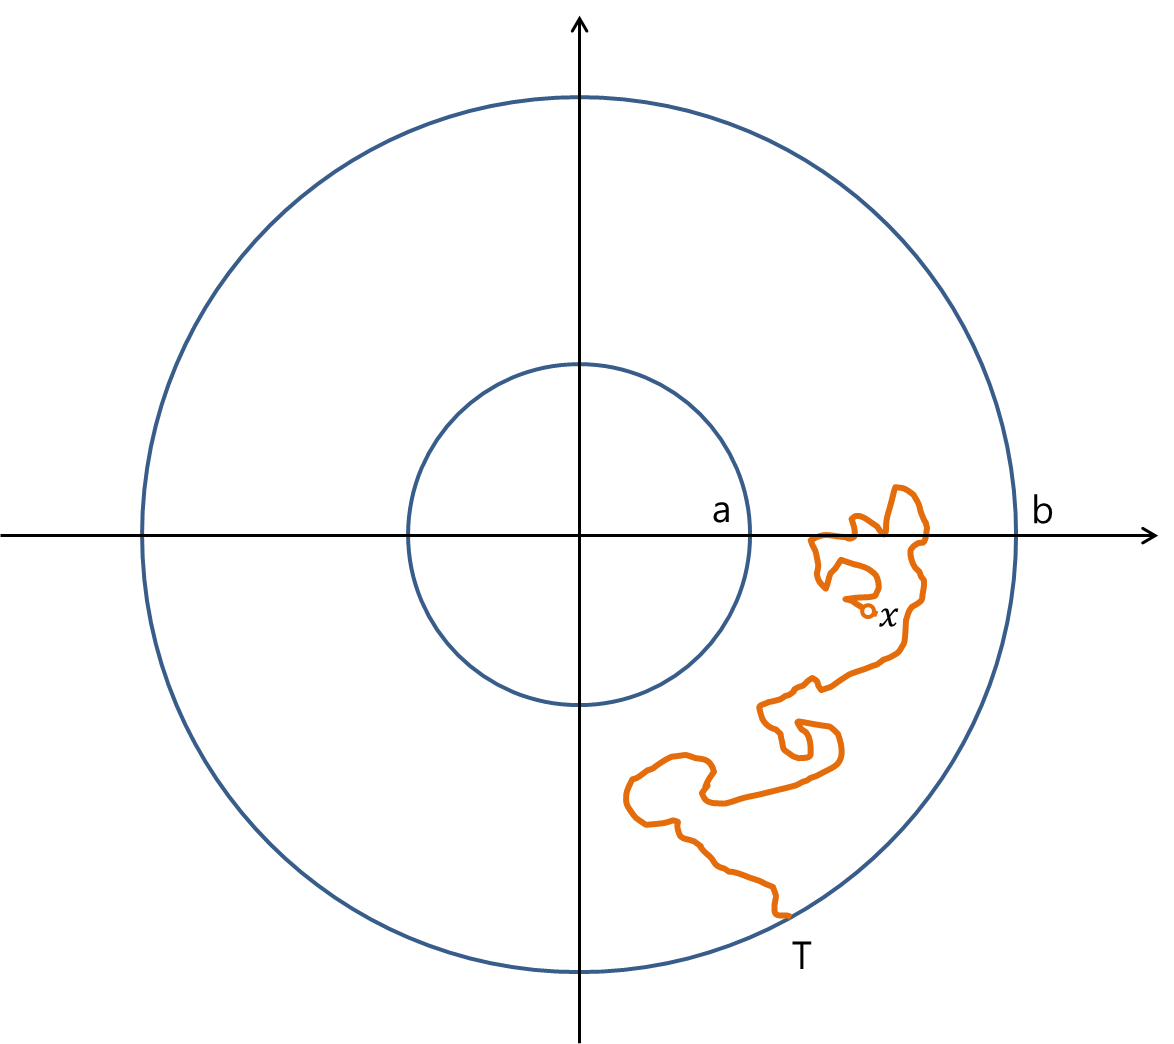
\includegraphics[width=0.33\textwidth]{2}
\end{figure}
Note that $\prob (T< \infty ) =1$. Also for $t\leq T$, $M_t = \log |X_t|$ so $M$ is bounded up to $T$. So optional stopping theorem applies to show
\begin{align*}
0 = \avg (M_0) = \avg(M_T) = \avg( \log |X_t|) = p\log a + (1-b) \log b
\end{align*}
where $p = p(a,b) =\prob (|X_T| =a)$. Consider the limit $a\rightarrow 0$, then $\log a \rightarrow -\infty$, so $p\rightarrow 0$. Hence for $|x|=1$, $p_0(x) = \lim_{b\rightarrow \infty} \lim_{a\rightarrow 0} p(a,b) =0$. By scaling, we see $p_0(x) =0$ for all $x\neq 0$.

\quad In the case $x=0$, for $n\in \mathbb{N}$, by Markov property,
\begin{align*}
\prob (|X_t| =0 \text{ for some }  t \geq \frac{1}{n}) = \int_{\reals^2} p(\frac{1}{n},0,y) p_0(y) dy =0
\end{align*} 
Let $n\rightarrow \infty$ to see $p_0(0) =0$.
\s

For $|x|=1$, let $b\rightarrow \infty$ with $a= \epsilon$ fixed. Since $\log b \rightarrow \infty$, $p(a,b)  \rightarrow 1$ so
\begin{align*}
p_{\epsilon} (x) = \lim_{b\rightarrow \infty} p(\epsilon, b)=1.
\end{align*}
By scaling $p_{\epsilon}(x) =1$ for all $x\neq 0$.

\quad If $x=0$, for $n\in \mathbb{N}$, by Markov property
\begin{align*}
\prob(|X_t| \leq \epsilon \text{ for some } t\geq n) = \int_{\reals^2} p(n,x,y) p_{\epsilon}(y) dy =1
\end{align*}
Hence $\prob(\{ t\geq 0, |X_t| \leq \epsilon \}$ is unbounded $)=1$.
\item[(c)] It will suffice to consider case $d=3$ and to show for all $N\in \mathbb{N}$ that
\begin{align*}
\prob ( \{ t\geq 0 : |X_t| \leq N  \} \text{ is unbounded} ) =0
\end{align*}
We repeat the argument from (b) with $1/|x|$ in place of $\log (|x|)$ - in $d=3$, $1/|x|$ is the harmonic function on $\reals^3 \backslash \{ 0 \}$ - to obtain
\begin{align*}
\frac{p}{a} + \frac{1-p}{b} =1
\end{align*}
for $p = \prob(|X_T|=a)$ and $(X_T)_{t\geq 0} \sim \text{BM}_x (\reals^3)$, $|x|=1$. Let $b\rightarrow \infty$ to see 
\begin{align*}
\lim_{b\rightarrow \infty} p(a,b)  =\prob (|X_t| \leq a \text{ for some } t\geq 0) =a
\end{align*} 
By scaling, for $|x| = N+1$,
\begin{align*}
\prob( |X_t| \leq N \text{ for some } t\geq 0) = \frac{N}{N+1}
\end{align*}
Set $T_0 =0$ and for $k\geq 1$,
\begin{align*}
S_k = \inf \{ t\geq T_{k-1} : |X_t| = N+1 \}, \quad T_k = \inf \{ t \geq S_k : |X_t| =N \}
\end{align*}

Then
\begin{align*}
\prob( T_k < \infty) \leq \frac{N}{N+1} \prob (T_{k-1} < \infty) \leq \Big(\frac{N}{N+1} \Big)^k \rightarrow 0
\end{align*}
by strong Markov property and induction. Set $K = \sup \{ k : T_k < \infty  \}$. Then $K< \infty$ a.s. Now for all $k \geq 1$, on $\{T_{k-1} < \infty \}$, has $S_{k} < \infty$ a.s. Hence $S_{K+1} < \infty$ a.s. But on $\{S_{K+1} \leq \infty \}$, has $|X_t| >N$ for all $t\geq S_{K+1}$ hence $\prob( \{ t\geq 0 : |X_t | \leq N \}$ is unbounded $)= 0$.
\end{itemize}

\eop
\end{proof}

\subsection*{7.9. Brownian Motion and the Dirichlet Problem}

Let $D$ be a connected open set in $\reals^d$. Write $\partial D$ for the boundary. Let $c: D \rightarrow [0,\infty)$, $f: \partial D \rightarrow [0,\infty)$ be measurable functions. For $x\in \overline{D}$, let $(X_t)_{t\geq 0}$ be a Brownian motion starting at $x$.

\quad Define the \textbf{expected total cost} by
\begin{align*}
\phi(x) = \avg \Big( \int_0^T c(X_t) dt + f(X_T) 1_{t< \infty} \Big)
\end{align*}
where $T = \inf \{ t\geq 0 : X_t \not\in D \}$. By a

\quad By a \textbf{solution of the Dirichlet problem (in $D$ with data $c$ and $f$)}, we mean a function $\psi \in C(\overline{D}) \cap C^2 (D)$ such that
\begin{align*}
\begin{cases}
\begin{array}{ll}
-\frac{1}{2} \Delta \psi = c & \text{in } D \\
\psi = f & \text{on } \partial D
\end{array}
\end{cases}
\end{align*}
Accordingly, say $\psi$ is a \textbf{super-solution} if $-\frac{1}{2} \Delta \psi \geq c$, $\psi \geq f$, and call $\psi$ a \textbf{sub-solution} with inverse inequalities.

\quad Suppose $\psi \in C_b^2(\reals^d)$ restrict to a solution of Dirichlet problem on $D$. Consider the martingale (as in \textbf{Theorem 7.5.1})
\begin{align*}
M_t = \psi(X_t) - \psi(X_0) - \int_0^t \frac{1}{2} \Delta \psi (X_s) ds
\end{align*}
Suppose we could justify optional stopping theorem at $T$ and suppose $T< \infty $ a.s. Then
\begin{align*}
0 = \avg(M_0) = \avg(M_T) = \avg(\psi(X_T)) - \psi(x) - \avg(\int_0^T \frac{1}{2} \Delta \psi(X_s) ds)
\end{align*} 
so 
\begin{align*}
\psi(x) = \avg(f(X_T)) + \avg(\int_0^T c(X_s) ds) = \phi(x)
\end{align*}
We will spend time in exploring the condition in which this holds.
\s

\newday

(19th November, Monday)
\s

Settings from the last lecture : $D$ a connected open set $\subset \reals^d$, $c: D \rightarrow [0,\infty)$, $f: \partial D \rightarrow [0,\infty)$ measurable functions,
\begin{align*}
\phi(x) = \avg\Big[ \int_0^T c(X_t) dt + f(X_T) 1_{T<\infty} \Big]
\end{align*}
$(X_t)_{t\geq 0} \sim \text{BM}_x(\reals^d)$, $T= \inf \{ t\geq 0 : X_t \not\in D \}$, times spent in $B\subset D$ before leaving.
\s

\thmnum{7.9.2 (a)} Let $\psi$ be a \emph{non-negative super-solution} of the Dirichlet Problem(DP), $\psi \in C(\overline{D}) \cap C^2(D)$,
\begin{align*}
\begin{cases}
\begin{array}{ll}
-\frac{1}{2} \Delta \psi \geq c & \text{in } D \\
\psi \geq f & \text{on } \partial D
\end{array}
\end{cases}
\end{align*}
Then $\psi \geq \phi$.
\begin{proof}
\pf Clear that $\psi \geq \phi$ on $\partial D$. Fix $x\in D$ and $N\geq 1$ such that $x\in D_N = \{ y\in D : |y|<N, \text{dist}(y,\partial D) > 1/N \}$. There exists $g\in C_b^2(\reals^d)$ such that $g= \psi$ on $D_N$. Consider
\begin{align*}
M_t = g(X_t) - g(X_0) - \int_0^t \frac{1}{2} \Delta g(X_s) ds
\end{align*}
and $T_N =\inf \{ t\geq 0 : X_t \not\in D_N \}$. Then $M$ is a martingale. By the optional stopping theorem, has
\begin{align*}
0 = \avg(M_0) = \avg(M_{T_N \wedge t} ) = \avg(\psi(X_{T_N \wedge t})) - \psi(x) + \avg \Big[ \int_0^{T_N \wedge t} \Big(-\frac{1}{2} \Delta \psi \Big) (X_s) ds \Big]  \quad \cdots \cdots\cdots (\star)
\end{align*}
Consider the limit $N\rightarrow \infty$ and then $t\rightarrow \infty$. Then $T_N \wedge t \nearrow T$, hence
\begin{align*}
\avg \int_0^{T_N \wedge t} \Big(-\frac{1}{2} \Delta \psi \Big) (X_s) ds \geq \avg \int_0^{T_N \wedge t} c(X_s) ds \rightarrow \avg \int_0^T c(X_s) ds
\end{align*}
by monotone convergence. On $\{T < \infty \}$,
\begin{align*}
\psi( X_{T_N \wedge t}) \rightarrow \psi(X_T) \quad \text{a.s.}
\end{align*}
so sine $\psi \geq 0$, by Fatou's lemma,
\begin{align*}
\liminf \avg( \psi(X_{T_N \wedge t})) \geq \avg(\psi(X_T) 1_{T<\infty}) \geq \avg(f(X_T) 1_{T<\infty})
\end{align*}
So taking $\liminf$ in ($\star$), we see $\psi \geq \phi$.

\eop
\end{proof}
\s

\thmnum{7.9.2 (b)} Let $\psi$ be a \emph{non-negative bounded solution} of the Dirichlet Problem, $\psi \in C(\overline{D}) \cap C^2(D)$
\begin{align*}
\begin{cases}
\begin{array}{ll}
-\frac{1}{2} \Delta \psi = c & \text{in } D \\
\psi = f & \text{on } \partial D
\end{array}
\end{cases}
\end{align*}
and suppose that $\avg(\psi(X_t)1_{t<T}) \rightarrow 0$ as $t\rightarrow \infty$($\cdots (\dagger$)). Then $\psi = \phi$.

\textbf{Remark about the condition ($\dagger$) :} Since we assume $\psi$ bounded and
\begin{align*}
|\avg(\psi | X_t) 1_{t<T}| \leq \norms{\psi}{\infty} \prob(t< T)
\end{align*}
We see condition ($\dagger$) holds whenever $T< \infty$ a.s. for all starting points $x$. e.g. we're OK if ($d=1$ and $\partial D \neq \varnothing$) or ($d=2$ and $\reals^2 \backslash D$ contains an open ball) or ($d\geq 3$ and $D$ bounded).
\begin{proof}
\pf Clear that $\psi = \phi$ on $\partial D$. Fix $x\in D$ and $N\geq 1$ such that $x\in D_N = \{ y\in D : |y|<N, \text{dist}(y,\partial D) > 1/N \}$. There exists $g\in C_b^2(\reals^d)$ such that $g= \psi$ on $D_N$. Consider
\begin{align*}
M_t = g(X_t) - g(X_0) - \int_0^t \frac{1}{2} \Delta g(X_s) ds
\end{align*}
and $T_N =\inf \{ t\geq 0 : X_t \not\in D_N \}$. Then $M$ is a martingale. By the optional stopping theorem, has
\begin{align*}
0 = \avg(M_0) = \avg(M_{T_N \wedge t} ) = \avg(\psi(X_{T_N \wedge t})) - \psi(x) + \avg \Big[ \int_0^{T_N \wedge t} \Big(-\frac{1}{2} \Delta \psi \Big) (X_s) ds \Big]  \quad \cdots \cdots\cdots (\star)
\end{align*}
Consider the limit $N\rightarrow \infty$ and then $t\rightarrow \infty$. Then $T_N \wedge t \nearrow T$, hence
\begin{align*}
\avg \int_0^{T_N \wedge t} \Big(-\frac{1}{2} \Delta \psi\Big) (X_s) ds = \avg \int_0^{T_N \wedge t} c(X_s) ds \rightarrow \avg \int_0^T c(X_s) ds
\end{align*}
by monotone convergence. Now 
\begin{align*}
\avg(\psi (X_{T_N \wedge t})) = \avg( \psi(X_{T_N}) 1_{T_N \leq t} ) + \avg(\psi(X_t) 1_{t< T_N})
\end{align*}
We have, sine $\psi \in C(\overline{D})$,
\begin{align*}
\psi(X_{T_N}) 1_{T_N \leq t} \rightarrow \psi(X_T) 1_{T< \infty} \quad \text{a.s.}
\end{align*}
and since $\psi$ is bounded, by dominated convergence,
\begin{align*}
\avg \Big[ \psi(X_{T_N}) 1_{T_N \leq t} \Big] \rightarrow \avg (\psi(X_T) 1_{T<\infty}) = \avg (f(X_T) 1_{T<\infty})
\end{align*}
Also by the assumption
\begin{align*}
\lim_{N\rightarrow \infty} \avg (\psi(X_t) 1_{t< T_N}) = \avg(\psi(X_t) 1_{t<T}) \rightarrow 0 \quad \text{as } t\rightarrow \infty
\end{align*}
Take limit in ($\star$) to see $\psi = \phi$.
\eop
\end{proof}
\s

This theorem tells us about uniqueness of solution of the Dirichlet problem, but it does not say anything about existence of the solution. We are next going to examine this problem.
\s

\thmnum{7.9.2 (c).(I)} Assume $d\geq 3$ and $D= \reals^d$ and $c$ has compact support and $c\in C^2(D)$. Then $\phi \in C^2(\reals^d)$ and $-\frac{1}{2} \Delta \phi =c$.
\begin{proof}
\pf Suppose $g$ is continuous and of compact support on $\reals^d$. Note
\begin{align*}
P_t g(x) = \avg g(x+X_t) = \int_{\reals^d} (2\pi t)^{-d/2} e^{-|x-y|^2/2t} g(y) dy
\end{align*}
where $(X_t)_{t\geq 0} \sim \text{BM}(\reals^d)$ so 
\begin{align*}
\begin{cases}
\norms{P_t g}{\infty}  \leq \norms{g}{\infty} \quad \text{\emph{and also}} \\
\norms{P_t g}{\infty} \leq (2\pi t)^{-d/2} \text{vol}(\text{supp}(g)) \norms{g}{\infty}
\end{cases} \quad \cdots \cdots\cdots (\diamond)
\end{align*}
So splitting the integral at 1 gives
\begin{align*}
\avg \int_0^{\infty} g(x+X_t) dt = \int_0^{\infty} P_t g(x) dt \leq (1+ \text{vol}(\text{supp}(g))) \norms{g}{\infty}
\end{align*}
Hence also for $\epsilon >0$,
\begin{align*}
\avg \int_0^{\infty} \sup_{|x-y|< \epsilon} |g(y+X_t)| dt < \infty
\end{align*}
(note, $g_{\epsilon}(x) = \sup_{|y-x| < \epsilon } |g(y)|$ is also continuous of compact support.) Now we can apply this to and its derivative to justify differentiating
\begin{align*}
\phi(x) = \avg \int_0^{\infty} c(x+X_t) dt
\end{align*}
under the integrals to obtain $\phi \in C^2(D)$ and 
\begin{align*}
\Delta  \phi(x) = \avg \int_0^{\infty} \Delta c(x+X_t) dt = \Big( \int_0^s + \int_s^t + \int_t^{\infty} \Big) \avg(\Delta c(x+X_r)) dr
\end{align*} 
for $0<s<t$. Consider the limits $s\rightarrow 0$ and $t\rightarrow \infty$. First and the third integrals tend to 0 using the estimates above. Now
\begin{align*}
\frac{1}{2} \int_s^t  \avg(\Delta c(x+X_r)) dr &= \frac{1}{2} \int_s^t \int_{\reals^d} \Delta c(y) p(r,x,y) dydr \\
&= \frac{1}{2} \int_s^t \int_{\reals^d} c(y) \Delta p(t,x,y) dy dr \\
& = \int_s^t \int_{\reals^d} c(y) \dot{p} (r,x,y) dydr \\
&= \int_{\reals^d} c(y) (p(t,x,y)-p(s,x,y)) dy \quad (\text{FTC})
\end{align*}
But $\int c(y) p(t,x,y) dy \rightarrow 0$ as $t\rightarrow \infty$ and $\int c(y)p(s,x,y) dy = \avg (c(x+X_s)) \rightarrow c(x)$ as $s\rightarrow 0$. Hence $-\frac{1}{2} \Delta \phi =c$ as required.

\eop 
\end{proof}
\s

\newday

(21st November, Wednesday)
\s

(part iii drop-in hours tomorrow 10:30 - 12:30).

(Bring a few different colored pens to class on Friday, if possible)

(Office hours on Monday, time and place TBD)
\s

\thmnum{7.9.4} Let $D$ be a connected open set $\subset \reals^d$ and let $\phi$ be a \emph{non-negative} measurable function on $D$. Suppose
\begin{align*}
\phi(x) = \int_{S(x,p)} \phi(y) \sigma_{x,p}(dy)
\end{align*}
whenever $B(x,p) \subset D$ where $\sigma_{x,p}$ is the uniform distribution on $S(x,p) = \{ y : |x-y| =p \}$. Then \emph{either} $\phi(x) = \infty$ for all $x$ \emph{or} $\phi \in C^{\infty}(D)$ with $\Delta \phi =0$.
\s

This would not be examinable, and will not be proved in the lecture - see online notes for proof.
\s

\thmnum{7.9.5} \emph{(Blumenthal's zero-one law)} Let $(X_t)_{t\geq 0} \sim \text{BM}_x(\reals^d)$. Then for all $A\in \F_{0+}^{X} = \bigcap_{t>0} \F_{t}^X$, has $\prob(A) \in \{ 0,1\}$.
\begin{proof}
\pf Consider the $\pi$-system $\mathscr{A} = \bigcup_{s>0} \sigma (X_t - X_s : t\geq s)$. Then for all $A_0 \in \F_{0+}^X$ and all $A \in \mathscr{A}$, we have $\prob(A_0 \cap A) = \prob(A_0) \prob(A)$. By Dynkin's lemma, this extend to all $A\in \sigma(\mathscr{A})$ (check details).

Now for all $s>0, t\geq s$, $X_t - X_s$ is $\sigma(\mathscr{A})$-measurable. But $X_s \rightarrow 0$ as $s\rightarrow 0$, so $X_t$ is $\sigma(\mathscr{A})$-measurable. So $\F_{\infty}^X = \sigma(\mathscr{A}) \supset \F_{0+}^X$. So for $A\in \F_{0+}^X$,
\begin{align*}
\prob(A) = \prob(A\cap A) = \prob(A)\prob(A)
\end{align*}
and therefore $\prob(A) \in \{0,1\}$.

\eop
\end{proof}
\s

\propnum{7.9.6} \emph{(Brownian motion enters all cones immediately)} Let $A$ be an open subset of $S^{d-1}$ and let $\epsilon>0$. Set $C$ a cone,
\begin{align*}
C = \{ty : y\in A, t\in (0,\epsilon) \}
\end{align*} 
Let $X \sim \text{BM}_0(\reals^d)$, and define $T_C = \inf \{ t\geq 0: X_t \in T_C \}$. Then $\prob(T_C =0)=1$. 
\begin{proof}
See example sheet.
\end{proof}
\s

Some definition (\textbf{External cone condition, ECC))} : Let $D \subset \reals^d$ be open and connected. Then $D$ satisfies ECC if for all $x\in \partial D$ , there exist $A$ open $\subset S^{d-1}$, $\epsilon >0$ such that
\begin{align*}
\{x+ty : t\in (0,\epsilon), y\in A \} \cap D = \phi
\end{align*}
This is weaker than the Lipschitz boundary condition.

\s
\thmnum{7.9.2(c)} Let $D$ be a connected open set $\subset \reals^d$. Let $c\in C^2(\reals^d)$, $f\in C(\partial D)$. Set
\begin{align*}
\phi(x) = \avg \Big( \int_0^T c(X_t) dt + f(X_T) 1_{T<\infty} \Big) \quad \forall x\in \overline{D}
\end{align*}
where $X \sim \text{BM}_x(\reals^d)$ and $T = \inf \{ t\geq 0: X_t \not\in D \}$. Assume $D$ satisfies the \emph{external cone condition(ECC)} and that $\phi$ is locally bounded. Then $\phi \in C^2(D) \cap C(\overline{D})$ and $-\frac{1}{2}\Delta \phi =c$ in $D$ and $\phi =f$ on $\partial D$. i.e. $\phi$ solves the Dirichlet condition.
\s

This is significant - the proof using ECC is hard to achieve just using usual theories of partial differential equations.(recall, we usually prove theorems under Lipschitz boundary condition in PDEs). Probability wins!
\s

\lemnum{7.9.3} Let $D_0$ be a \emph{bounded subset} of $D$. Define $T_0 = \inf \{t\geq 0: X_t \not\in D_0 \}$, $x\in \overline{D}$. Then
\begin{align*}
\phi(x) = \avg \Big( \int_0^{T_0} c(X_t) dt + \phi(X_{T_{0}}) \Big)
\end{align*}
\begin{proof}
\pf Set $\tilde{X}_t = X_{T_0 +t}$, $\tilde{\F}_{t} = \F_{T_0 +t}$, and $\tilde{T} = \inf \{ t\geq 0 : \tilde{X}_t \not\in D \}$. By \emph{Strong Markov property}, $(\tilde{X}_t)$ is an $(\tilde{\F}_t)$-BM. Now
\begin{align*}
\int_0^T c(X_t) dt + f(X_T) 1_{T<\infty} = \int_0^{T_0} c(X_t) dt + \int_0^{\tilde{T}} c(\tilde{X}_t) dt + f(\tilde{X}_{\tilde{T}})1_{\tilde{T}<\infty} \quad \cdots\cdots\cdots (\dagger)
\end{align*}
Here we used that $\tilde{T}<\infty$ \emph{iff} $T<\infty$ and $X_T = \tilde{X}_{\tilde{T}}$. By \textbf{Prop 7.4.1},
\begin{align*}
\avg( \int_0^{\tilde{T}} c(\tilde{X}_t) dt + f(\tilde{X}_{\tilde{T}})1_{\tilde{T}<\infty} | \F_{T_0} ) = \phi(X_{T_0}) \quad \text{a.s.}
\end{align*}
So we obtain result on taking $\avg$ in ($\dagger$)

\eop
\end{proof}
\s

Recall, we proved \textbf{Theorem 7.9.2(c)} in a weaker setting earlier. Here, we prove in a slightly more general setting.
\begin{proof}
\textbf{proof of Theorem 7.9.2(c) II.} We show in the case $c=0$ that $\phi \in C^{\infty}(D)$ with $\Delta \phi =0$ -then follows from a simple argument using symmetry of a sphere and \textbf{Theorem 7.9.4}.

See online notes.
\end{proof}
\s

\begin{proof}
\textbf{proof of Theorem 7.9.2(c) III.} Given the setting of the theorem, we show for all $y \in \partial D$ that
\begin{align*}
\lim_{x\rightarrow y, x\in \overline{D}} \phi(x) = f(y)
\end{align*}
Fix $y\in \partial D$ and choose $U$ bounded open set $\subset \reals^d$ with $u\in U$ be such that $y\in D_0=D\cap U$. By \emph{exterior cone condition}, there exist $A\in S^{d-1}$, $\epsilon>0$ such that $\{y+tz : t \in (0,\epsilon) , z\in A \} \cap D = \phi$. Let $(X_t)_{t\geq 0}$ be a $\text{BM}_0(\reals^d)$. Set $T_0(x) = \inf \{ t\geq 0: x+ X_t \not\in D \}$. By \textbf{Proposition 7.9.6}, for $T_C = \inf \{t\geq 0 : y+X_t \in C \}$ we have $T_C =0$ a.s. Now on the event $\{ T_C =0 \}$, we have $T_0(x) \rightarrow 0$ as $x\rightarrow y$($x$ staying in $\overline{D}$) so $X_{T_0(x)} + x \in \partial D$ eventually as $x\rightarrow y$ and $X_{T_0(x)} +x \rightarrow y$ as $x\rightarrow y$. Hence
\begin{align*}
\phi(X_{T_0(x)} +x) = f(X_{T_0(x)} +x) \rightarrow f(y) \quad \text{as }x\rightarrow y
\end{align*}
Also by \textbf{Prop 7.7.1}, $\avg(\sup_{x\in D_0} T_0(x)) < \infty$. Now
\begin{align*}
\phi(x) = \avg \Big( \int_0^{T_0(x)} c(x+X_t)dt + \phi(X_{T_0(x)} + x) \Big)
\end{align*}
Let $x\rightarrow y$, then using dominated convergence to see $\phi(x) \rightarrow f(y)$ as $x\rightarrow y$.

\eop
\end{proof}
\s

\newday

(23rd November, Friday)
\s

The following is the last part of proof of \textbf{Theorem 7.9.2(c)}
\s

\begin{proof}
\textbf{\textbf{proof of Theorem 7.9.2(c) IV.}} It will suffice to consider the case where $d\geq 3$, or set $\tilde{D} = D \times \reals^2$ and extend $c$ as a constant in new directions. 

\quad Consider for now the case $D$ bounded. There exists $\tilde{c} \in C^2(\reals^d)$ of compact support with $\tilde{c} = c$ in $D$. Set
\begin{align*}
\phi_0(x) = \avg \int_0^{\infty} \tilde{c}(X_t) dt
\end{align*}
By \textbf{part I}, $\phi_0 \in C^2(\reals^d)$ with $-\frac{1}{2}\Delta \phi_0 = \tilde{c}$. Now
\begin{align*}
\phi_0(x) = \avg \Big( \int_0^T \tilde{c}(X_t) dt + \phi_0(X_T) \Big) = \phi(x) + \phi_1(x)
\end{align*}
(by \textbf{Lemma 7.9.3}) where $\phi_1(x)  = \avg(\phi_0(X_T))$. By \textbf{part II}, $\phi_1 \in C^{\infty}(D)$ and $\Delta \phi_1 =0$. So $\phi \in C^2 (D)$ and $-\frac{1}{2} \Delta \phi =c$.

\quad Turn to the case $D$ unbounded. Choose any bounded open $D_0 \subset D$. Then
\begin{align*}
\phi (x) = \phi_0(x) + \phi_1(x)
\end{align*}
(new $\phi_0$ and $\phi_1$) where $\phi_0$ and $\phi_1$ are defined by
\begin{align*}
\phi_0(x) = \avg \Big( \int_0^{T_0} c(X_t) dt \Big), \quad \phi_1(x) = \avg(\phi(X_{T_0}))
\end{align*}
where $T_0  = \inf \{ t\geq 0 : X_t \not\in D_0 \}$. We know $\phi_0 \in C^2(D)$ and $-\frac{1}{2}\Delta \phi_0 = c$ and since $\phi$ is locally bounded, $\phi_1 \in C^{\infty}(D_0)$ with $\Delta \phi_1 =0$. Hence $\phi \in C^2(D_0)$ and $-\frac{1}{2}\Delta \phi =c$.

\eop
\end{proof}
\s

Plan for the rest of the course : we will not cover all the materials(e.g. Donsker's invariance principle or Skorohod embedding for random walks) - do not have enough time. But will discuss about Poisson random measures.

\section*{8. Poisson Random Measures}

Our ambition is to classify all stationary independent increments - this is what L\'{e}vy-Khinchin theorem tells us. To prove this, we need some works on Poisson random measures.

\subsection*{8.1. Construction}

For $\lambda \in (0,\infty)$, a random variable $X$ with values in $\mathbb{Z}^+ \cup \{\infty \}$ has distribution $P(\lambda)$ if
\begin{align*}
\prob(X = x) = e^{-\lambda} \frac{\lambda^x}{x!}, \quad x\in \mathbb{Z}^+
\end{align*}
Also conventionally write $X \sim P(0)$ if $X \equiv 0$, and $P \sim P(\infty) $ if $X \equiv \infty$.
\s

\propnum{8.1.1.}\emph{(Addition property)} Let $(N_k : k\in \mathbb{N})$ be a sequence of independent random variables with $N_k \sim P(\lambda_k)$ for all $k$. Then 
\begin{align*}
\sum_{k} N_k \sim P \big( \sum_k \lambda_k \big)
\end{align*}
\s

\propnum{8.1.2.}\emph{(Splitting property)} Suppose $N\sim P(\lambda)$. Let $(Y_n : n\in \mathbb{N})$ be a sequence of i.i.d. random variables in $\mathbb{N}$. Set $N_k = \sum_{n=1}^N 1_{Y_n =k}$ for $k\geq 1$. Then $(N_k : k\in \mathbb{N})$ is a sequence of independent $P(\lambda_k)$ random variables with $\lambda_k = \lambda \prob(Y_1 =k)$.
\s

The proofs are just elementary calculations, but please do them!!!
\s

Let $(E, \mathscr{E}, \mu)$ be a \emph{$\sigma$-finite} measure space.

\begin{itemize}
\item A \textbf{Poisson random measure} of intensity $\mu$ is a map $M : \Omega \times \mathscr{E} \rightarrow \mathbb{Z}^+ \cup \{\infty \}$ (for $A \in \mathscr{E}$, think of $M(A)$ as $M(\{\omega \} \times A)$, a random variable) such that for any disjoint sequence $(A_k : k\in \mathbb{N})$ in $\mathscr{E}$,
\begin{itemize}
\item[(i)] $M(\cup_k A_k) = \sum_k M(A_k)$. 
\item[(ii)] $M(A_k)$ is a $P(\mu(A_k))$ random variable for all $k$.
\item[(iii)] The random variables $M(A_k)$, $k\in \mathbb{N}$ are independent.
\end{itemize}
\item We can construct a $\text{PRM}(\mu)$ as follows.

\quad First in case $\mu(E) < \infty$, take $N\sim P(\lambda)$, $\lambda = \mu(E)$ and take independent random variables $(Y_n : n\in \mathbb{N})$ independent of $N$ with distribution $\frac{1}{\lambda} \mu$. Define $M(A) = \sum_{n=1}^{N} 1_{Y_n \in A}$ Then $M \sim \text{PRM}(\mu)$, i.e. $M(A) \sim P(\mu(A))$. (\textbf{an exercise})

\quad In general, if $\mu(E) = \infty$, as $E$ is $\sigma$-finite, there exist disjoint $E_n \in \mathscr{E}$ with $\cup_{n} E_{n} = E$ such that $\mu(E_n) < \infty$ for all $n$. Using preceding construction, we obtain $(M_n)_n$ independent $\text{PRM}(\mu 1_{E_n})$'s. Then set $M = \sum_n M_n$. Then $M \sim \text{PRM}(\mu)$. (\textbf{also an exercise})

\item The uniqueness of such map also can be shown - refer to the online lecture notes.
\end{itemize}

\subsection*{8.2. Integrals with respect to Poisson Random Measures}

\thmnum{8.2.1} Let $M$ be a $\text{PRM}(\mu)$ and let $g$ be a measurable function on $(E, \mathscr{E})$. Assume $\mu(E) < \infty$. Define
\begin{align*}
M(g) = \begin{cases}
\begin{array}{ll}
\int_E g(y) M(dy) & \text{if  } M(E) < \infty \\
0 & \text{o/w}
\end{array}
\end{cases}
\end{align*}
Then $M(g)$ is a well-defined random variable and 
\begin{align*}
\avg(e^{inM(g)}) = \exp \Big[ \int_E (e^{ing(y)} -1) \mu(dy) \Big]
\end{align*}
and if $g\in L^1(\mu)$ then $M(g) \in L^1(\prob)$ with $\avg(M(g)) = \mu(g)$ and $\text{Var}(M(g)) = \mu(g^2)$.
\begin{proof}
\pf Let's see these all true in the case $M(A) = \sum_{n=1}^N 1_{Y_n \in A}$. Then $M(g) = \sum_{n=1}^N g(Y_n)$ and this is clearly a well-defined measurable function. We have
\begin{align*}
\avg(e^{in M(g)} | N=n) = \avg( e^{in \sum_{k=1}^n g(Y_k) }) =\prod_{k=1}^n \avg( e^{in  g(Y_k) }) = \Big( \int_E e^{in g(y)} \frac{\mu(dy)}{\lambda} \Big)^n
\end{align*}
So 
\begin{align*}
\avg(e^{in M(g)}) &= \sum_{n=0}^{\infty} e^{-\lambda} \frac{\lambda^n}{n!} \Big( \int_E e^{ing(y)} \frac{\mu(dy)}{\lambda} \Big)^n \\
&= e^{-\lambda} \exp \Big( \int_E e^{ing(y)} \mu(dy) \Big)
\end{align*}
so we obtain the average and variance of $M(g)$ from the moment generating function.

\quad For the general case, since $(E, \mathscr{E},\mu)$ is $\sigma$-finite, let $E = \cup_n E_n$ where $E_n \in \mathscr{E}$, disjoint and $\mu(E_n) < \infty$. Let $M_n$ be the Poisson random measure on each $E_n$. Then $1_{M<\infty} \sum_{n=1}^{m} M_{n} \rightarrow M 1_{M<\infty}$ as $m\rightarrow \infty$. The statement holds for each $M_n$ by above, so by dominated convergence(dominated by 1),
\begin{align*}
\avg(e^{in M(g)}) &= \sum_{n=0}^{\infty} e^{-\lambda} \frac{\lambda^n}{n!} \Big( \int_E e^{ing(y)} \frac{\mu(dy)}{\lambda} \Big)^n \\
&= e^{-\lambda} \exp \Big( \int_E e^{ing(y)} \mu(dy) \Big)
\end{align*}
also holds.

\eop
\end{proof}
\s

\newday

(26th November, Monday)
\s

Last time : $(E,\mathscr{E},\mu)$, then $M : \Omega \times \mathscr{E} \rightarrow \mathbb{Z}^+ \cup \{\infty\}$. Then $M\sim \text{PRM}(\mu)$ if for any $(A_k : k\in \mathbb{N})$ in $\mathscr{E}$ \emph{disjoint},
\begin{itemize}
\item[(i)] $M(\cup_k A_k) = \sum_k M(A_k)$. 
\item[(ii)] $M(A_k)$ is a $P(\mu(A_k))$ random variable for all $k$.
\item[(iii)] The random variables $M(A_k)$, $k\in \mathbb{N}$ are independent.
\end{itemize}
If $\mu(E) =\lambda < \infty$, $M(A) = \sum_{k=1}^N 1_{Y_k \in A}$ with $N\sim P(\lambda)$, $(Y_n : n\in \mathbb{N})$ i.i.d $\sim \frac{1}{\lambda
}\mu$. Also, $M(g) = \sum_{n=1}^N g(Y_n)$, for $g: E \rightarrow \reals$, $\avg(M(g)) = \mu(g)$, $\text{Var}(M(g)) = \mu (g^2)$, and $\avg(e^{inM(g)}) = \exp \int_E (e^{ing(y)}-1) \mu(dy)$.
\s

Now we want to introduce time to this construction. Let $(E, \mathscr{E} , K)$ be a $\sigma$-finite measure space. Then let $\mu = dt \otimes K$ on $(0, \infty) \times E$. Let $M$ be a $\text{PRM}$ on $(0,\infty) \times E$ with intensity $\mu$. Write $\tilde{M} = M-\mu$. Call $\tilde{M}$ a \textbf{compensated Poisson Random Measure.} Use filtration $(\F_t)_{t\geq 0}$, $\F_t = \sigma (\F_t^M, \mathscr{N})$ where $\F_t^M = \sigma \big( M([0,s) \times A ) : s\leq t, A\in \mathscr{E} \big)$ and $\mathscr{N} = \{B\in \F_{\infty}^M : P(B) =0\}$ is the set of null sets.
\s

Similarly as above, can use, for case $K(E)<\infty$, that $M_t(g) = \sum_{n=1}^{N_t} g(Y_n)$ for $N \sim \text{PP}(\lambda)$, $g: E\rightarrow \reals$.
\s

\propnum{8.2.2} Assume $K(E) < \infty$ and $g\in L^1(K)$. Set
\begin{align*}
\tilde{M}_t(g) = \begin{cases}
\begin{array}{ll}
\int_{(0,t] \times E} g(y) \tilde{M} (ds,dy) & \text{if }  \mu( (0,t] \times E) < \infty \,\, \forall t\geq 0 \\
0 & \text{otherwise}
\end{array}
\end{cases}
\end{align*}
Then $(\tilde{M}_t(g))_{t\geq 0}$ is a \emph{cadlag martingale} with \emph{stationary independent increments}. Moreover,
\begin{align*}
\begin{array}{ll}
\avg(\tilde{M}_t(g)^2) = t\int_E g(y)^2 K(dy) & \cdots\cdots\cdots (\heartsuit) \\
\avg(e^{iu\tilde{M}_t(g)}) =\exp\Big[ t\int_E (e^{iug(y)}-1) K(dy) \Big] & \cdots\cdots\cdots (\oplus)
\end{array}
\end{align*}
\begin{proof}
\pf Exercise.
\end{proof}
\s

This can be thought of a sort of pre-view of what we do in stochastic calculus course, in which we use Gaussian random variables instead of Poissons.
\s

\thmnum{8.2.3} Let $g\in L^2(K)$. Take $E_n \in \mathscr{E}$ with $E_n \nearrow E$ and $K(E_n) < \infty$. Set $X_t^n = \tilde{M}_t(g1_{E_n})$. Then there exists a \emph{cadlag martingale} $(X_t)_{t\geq 0}$ such that $\avg(\sup_{s\leq t} |X_s^n - X_s|^2) \rightarrow 0$ as $n\rightarrow \infty$ for all $t\geq 0$. 

\quad Define $\tilde{M}_t(g) = X_t$. Then $(\tilde{M}_t(g))_{t\geq 0}$ has \emph{stationary independent increments} and ($\heartsuit$) and $(\oplus)$ still hold - so we may write, in convention,
\begin{align*}
\tilde{M}_t(g) = \int_{(0,t] \times E} g(y) \tilde{M}(ds,dy)
\end{align*}
and call $(\tilde{M}_t(g))_{t\geq 0}$ (a version of the stochastic) integral of $g$ with respect to $\tilde{M}$. (Although the integral does not converge absolutely!!!)
\begin{proof}
\pf For $n\leq m$,
\begin{align*}
\avg( |X^n_t - X^m_t|^2) = \avg( \tilde{M}_t(g1_{E_m \backslash E_n})^2) =  t\cdot \int_{E_m \backslash E_n} g(y)^2 K(dy) \rightarrow 0 \quad \text{(dominated convergence)}
\end{align*}\\
So by Doob's $L^2$-inequality,
\begin{align*}
\avg(\sup_{s\leq t} |X_s^n - X_s^m|^2) \leq 4\avg(|X_t^n - X_t^m|^2) \rightarrow 0 \quad \text{as } n,m\rightarrow \infty \quad \cdots\cdots\cdots (\otimes)
\end{align*}
So there exists $(n_k)$ such that
\begin{align*}
\sup_{s \leq t} |X_s^{n_k} - X_s^{n_j}| \rightarrow 0 \quad \text{a.s. as } j,k\rightarrow \infty 
\end{align*}
Since the uniform limit of cadlag function is cadlag, there exists a cadlag process $(X_t)_{t\geq 0}$ such that
\begin{align*}
\sup_{s\leq t} |X_s^{n_k} - X_s| \rightarrow 0 \quad \text{a.s. as } k \rightarrow \infty
\end{align*}
Note that $X_s \in L^2(\prob)$, because $X_t \leq X^0 + \sup_{n}(\sup_{s\leq t} (X_s^n - X^0))$. By Fatou's lemma with $(\otimes)$, has
\begin{align*}
\avg(\sup_{s\leq t} |X_s^n - X_s|^2 ) \rightarrow 0 \quad \text{as } n\rightarrow \infty
\end{align*}
Now for $A \in \F_s$, has
\begin{align*}
& \avg( (X_t^n - X_s^n) 1_A ) =0 \\
& \avg(e^{iu (X_t^n - X_s^n)} 1_A) = \prob(A) \times \exp \Big[ t\int_{E_n} (e^{iug(y)-1-ug(y)}) K(dy) \Big]
\end{align*}
But $X_t^n \rightarrow X_t$ in $L^2(\prob)$ for all $t$ so on letting $n\rightarrow \infty$ in these equations we see (using $|e^{iug}-1-iug| \leq \frac{1}{2}u^2 g^2)$)
\begin{align*}
& \avg( (X_t - X_s) 1_A ) =0 \\
& \avg(e^{in (X_t - X_s)} 1_A) = \prob(A) \times \exp \Big[ t\int_{n} (e^{iug(y)-1-ug(y)}) K(dy) \Big]
\end{align*}
so $(X_t)_{t\geq 0}$ is a martingale and both $(\heartsuit)$ and $(\oplus)$ hold and $(X_t)_{t\geq 0}$ has stationary independent increments.\\

\eop
\end{proof}

\section*{9. L\'{e}vy Processes}

\subsection{9.1. Definitions}

A \textbf{L\'{e}vy process} is a cadlag process with stationary independent increments starting at 0. Say that $(a,b,K)$ is a \textbf{L\'{e}vy triple} if $a\in [0,\infty)$, $b\in \reals$ and $K$ is a Borel measure on $\reals$ with $K(\{0\}) =0$ and
\begin{align*}
\int_{\reals} (|y|^2 \wedge 1) K(dy) < \infty
\end{align*}
We call $a$ the \textbf{diffusivity}, $b$ the \textbf{drift} and $K$ the \textbf{L\'{e}vy measure}. These notions generalize naturally to processes with values in $\reals^d$ but we will consider only the case $d = 1$. Take a Brownian motion $(B_t)$ and a Poisson random measure $M$ on $(0,\infty) \times \reals$ of intensity $\mu = dt \otimes K$. Set
\begin{align*}
X_t = bt + \sqrt{a} B_t +\int_{(0,t]\times \reals} y1_{|y| \leq 1} \tilde{M}(ds,dy) + \int_{(0,t] \times \reals} y1_{|y|>1} M(ds,dy)
\end{align*}
Note that the first integral exists because $|y|\wedge 1 \in L^2(K)$ and the second integral exists because $\mu((0,t] \times \{y: |y|\geq 1\}   ) < \infty$. Now putting the results from \textbf{Section 8} together, we see that, $(X_t)$ is \emph{cadlag with stationary independent increments} and
\begin{align*}
\avg(e^{iu X_t}) = e^{t\psi_{a,b,K}(u)}
\end{align*}
where $\psi_{a,b,K}(u) = iub - \frac{1}{2}u^2a  + \int_E (e^{iuy} - 1 - iuy1_{|y|\leq 1}) K(dy)$. Thus, to every L\'{e}vy triple there corresponds a L\'{e}vy process.
\s

\newday

(28th November, Wednesday)

\subsection*{9.2. L\'{e}vy-Khinchine Theorem}

\thmnum{9.2.1} Let $(X_t)_{t\geq 0}$ be a L\'{e}vy process (i.e. cadlag, stationary independent increments with $X_0=0$.) Then there exists a L\'{e}vy triple $(a,b,K)$ such that $\avg(e^{iuX_t}) = e^{t\psi(u)}$ for all $t\geq 0$, $u \in \reals$ where
\begin{align*}
\psi(u) \equiv \psi_{a,b,K}(u) =ibu - \frac{1}{2}au^2 + \int_{\reals} (e^{iuy}-1-iuy 1_{|y|\leq 1}) K(dy)
\end{align*}
and $\int_{\reals} (1\wedge |y|^2) K(dy) < \infty$.
\begin{proof}
\pf
\begin{itemize}
\item[I.] Set $\phi_t(y) = \avg(e^{iuX_t})$. We'll show $\phi_t(y) = e^{t\psi(u)}$ for some $\psi : \reals \rightarrow \mathbb{C}$ continuous.

\quad First note $\phi_t : \reals \rightarrow \mathbb{C}$ is continuous. Since $X$ has stationary independent increments and
\begin{align*}
X_{nt} = X_t + (X_{2t} - X_t) + \cdots + (X_{nt}- X_{(n-1)t})
\end{align*}
so we have $\phi_{nt}(u) = (\phi_t(u))^n$. Since $X$ is cadlag, for all $s\geq 0$, for $t>s$, has $X_t \rightarrow X_s$ as $t\rightarrow s$ so 
\begin{align*}
| \phi_t(u) - \phi_s(u)| \leq \avg (|e^{iu(X_t-X_s)} -1|) \leq \avg((u|X_t-X_s|\wedge 2))
\end{align*}
So $\phi_t(u) \rightarrow \phi_s(u)$ uniformly in $u$ on compact domains. Since $X_0 =0$, $\phi_0(u)=1$, now $|\phi_t(u)|^{1/n} = |\phi_{t/n}(u)| \rightarrow 1$ so $\phi_t(y) \neq 0$ for all $t\geq 0$, $u\in \reals$.

\begin{figure}[h]
	\begin{center}
		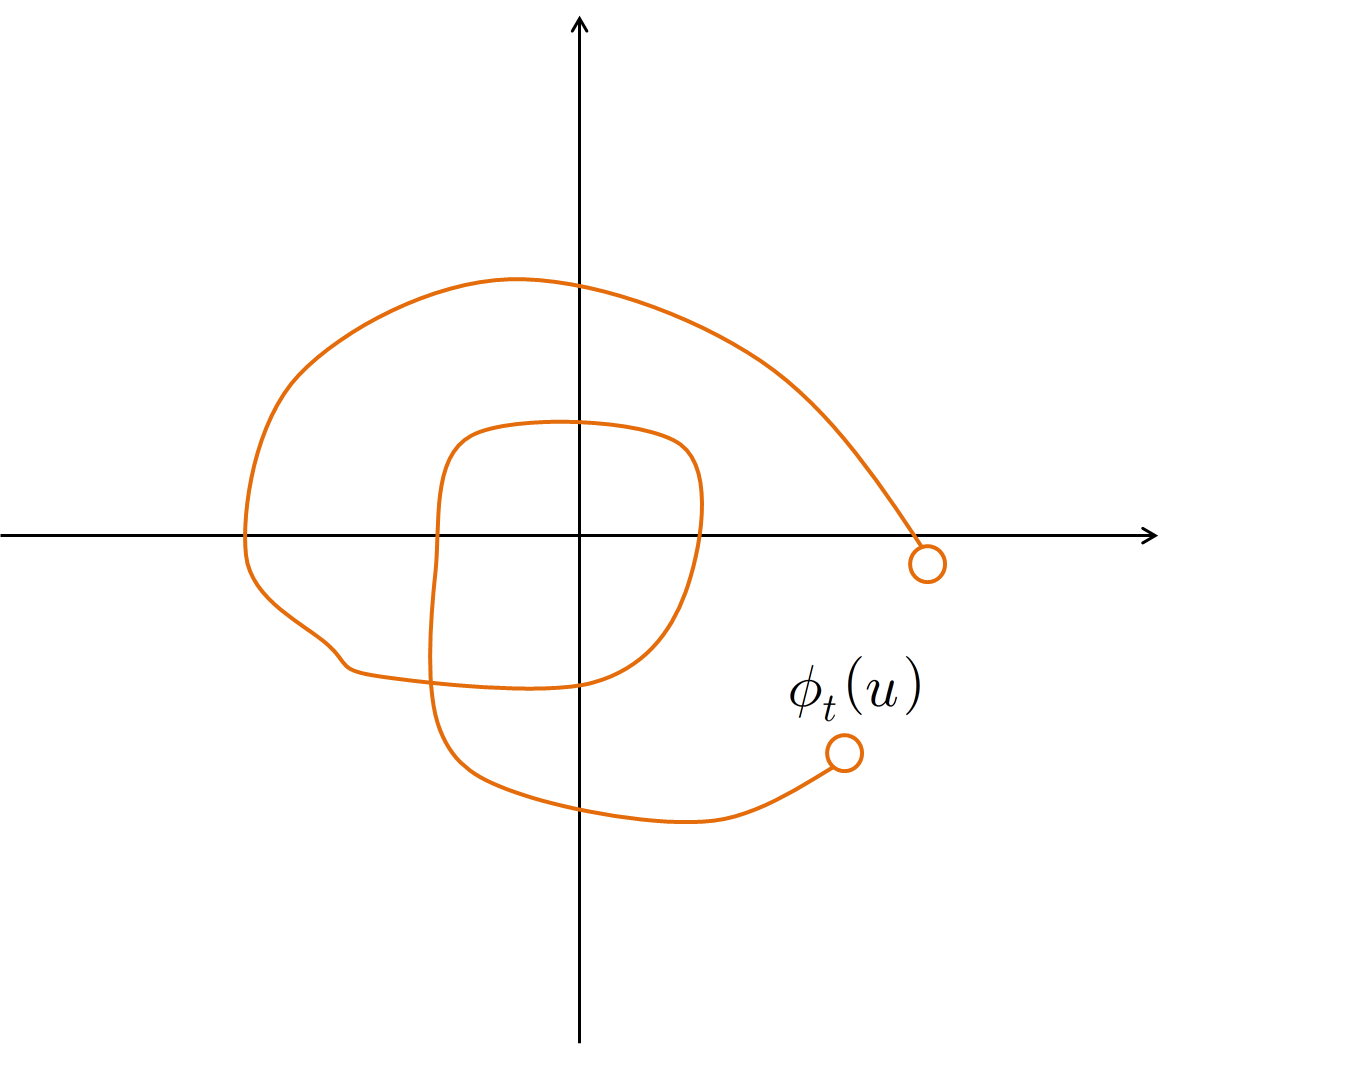
\includegraphics[scale=0.3]{3}
	\end{center}
\end{figure}
\quad Consider path $(\phi_t(r) : r\in [0,n])$. Define 
\begin{align*}
\psi_t(u) = \int_1^{\phi_t(u)} \frac{dz}{z}
\end{align*}
where we integrate along contour homotopic to the path $(\phi_t(r) : r\in [0,u])$ in $\mathbb{C} \backslash \{0 \}$. 
Then $\psi_t : \reals \rightarrow \mathbb{C}$ is continuous and
\begin{align*}
\phi_t(u) = e^{\psi_t(u)}
\end{align*}
Now $\psi_{nt}(u) = n\psi_t(u)$, $\psi_0(u) =0$, and $t\mapsto \psi_t(y)$ is right-continuous. Hence $\psi_t(u) = t\psi_1(u)$ for all $t\geq 0$ - so define $\psi$ to be $\psi =\psi_1$, then $\psi_t(u) = t\psi(u)$.
\item[II.] We produce a limit object.

Set $\nu_n =\text{law of }X_{1/n}$. Then
\begin{align*}
\psi(u) = \lim_{n\rightarrow \infty} n( \phi_{1/n}(u) -1)
\end{align*}
uniformly in $u$ on compact domains and $n(\phi_{1/n}(u)-1) = \int_{\reals} (e^{iuy}-1) n\nu_n(dy)$ so
\begin{align*}
\int_{\reals} (1-\cos (uy)) n\nu_n (dy) \rightarrow - \text{Re} \psi(u)
\end{align*}
uniformly in $u$ on compact domains. There exists $C< \infty$ such that
\begin{align*}
y^2 1_{|y|\leq 1} \leq C (1-\cos (u)) \quad \forall y \in \reals
\end{align*}
and also for all $\lambda >0$, has
\begin{align*}
1_{|y| \geq \lambda} \leq C\lambda \int_0^{1/\lambda} (1-\cos (uy)) du
\end{align*}
Set $\eta_n(dy) = n \nu_n (dy) (1\wedge y^2)$. Then integration gives 
\begin{align*}
\eta_n ([-1,1]) \leq \int_{\reals} C(1-\cos (y)) n\nu_n (dy) \rightarrow -C \cdot \text{Re}(\psi(1))
\end{align*}
and for $\lambda >1$
\begin{align*}
\eta_n (\reals \backslash (-\lambda, \lambda)) \leq & C \lambda \int_{\reals} \int_0^{1/\lambda} (1- \cos (uy))du \cdot n \nu_n(dy) \\
=& C\lambda \int_0^{1/\lambda} \int_{\reals} (1- \cos(uy)) n\nu_n (dy) du  \\
\xrightarrow{n\rightarrow \infty} &C \lambda \int_0^{1/\lambda} (-\text{Re}(\psi(u))) du
\end{align*}
Since $\psi(0)=0$ and $\psi$ continuous, this converges to 0 as $\lambda \rightarrow \infty$. Hence $(\eta_n : n\in \mathbb{N})$ is bounded in total mass and tight, so by Prohorov's theorem, there exists a finite Borel masure $\eta$ and a subsequence $(n_k)_k \subset \mathbb{N}$ such that $\eta_{n_k } \rightarrow \eta$ weakly.
\item[III.] Now divide $\psi$ into two parts by
\begin{align*}
\psi(u) &= \lim_{n\rightarrow \infty} \int_{\reals} \frac{(e^{iuy}-1)}{1\wedge |y|^2} \eta_n(dy) \\
&= \lim_{k\rightarrow \infty} (\int_{\reals} \mathscr{O}(u,y)\eta_{n_k}(dy)  + iu\beta_{n_k})
\end{align*}
where
\begin{align*}
\mathscr{O}(u,y) = \begin{cases}
\begin{array}{ll}
(e^{iuy}-1-iuy \chi(y)/(1\wedge y^2) & \text{if } y \neq 0\\
-u^2/2 & \text{if } y=0
\end{array}
\end{cases}
\end{align*}
$\chi : \reals \rightarrow [0,1]$ continuous, $1_{|y|\leq 1} \leq  \chi \leq 1_{|y|\leq 2}$ and
\begin{align*}
\beta_n = \int_{\reals} \frac{y \chi(y)}{1\wedge y^2} \cdot \eta_n (dy)
\end{align*}
Now $\mathscr{O}(u, \cdot) \in C_b(\reals)$ so $\int_{\reals} \mathscr{O}(u,y) \eta_{n_k} (dy)$ converges as $k\rightarrow \infty $ and in turn $\beta_{n_k}$ converges as $k\rightarrow \infty$, say $\beta_{n_k} \rightarrow \beta$ for some $\beta \in \reals$. Hence $\psi(u) = \psi_{a,b,K}(u)$ where
\begin{align*}
a &= \eta(\{0\}) \\
K(dy) &= 1_{y\neq 0} \eta(dy) / (1\wedge y^2) \\
b &= \beta - \int_{\reals} y \Big( \chi(y) - 1_{|y|\leq 1} \Big) K(dy)
\end{align*}
That is,
\begin{align*}
\psi(u) = iub - \frac{1}{2}u^2a  + \int_E (e^{iuy} - 1 - iuy1_{|y|\leq 1}) K(dy)
\end{align*}
\end{itemize}

\eop
\end{proof}

\end{document}